\documentclass[11pt]{report}


%%% fonts %%%
\usepackage{kpfonts}%  for math 
\usepackage{xgreek}
\usepackage{fontspec}
\setmainfont[Ligatures=TeX]{Linux Libertine O}
\usepackage{parskip}

%%% math %%%
\usepackage{amsmath}
\usepackage{mathtools}
\DeclarePairedDelimiter\floor{\lfloor}{\rfloor}
\DeclarePairedDelimiter\abs{\lvert}{\rvert}%
\makeatletter
\newcommand{\ssymbol}[1]{^{\@fnsymbol{#1}}}
\makeatother
\newcommand\inv[1]{#1\raisebox{1.15ex}{$\scriptscriptstyle-\!1$}}
\newcommand{\norm}[1]{\left\lVert#1\right\rVert}
\DeclareMathOperator*{\argmin}{arg\,min}

%%%% images %%%
\usepackage{graphicx}
\graphicspath{ {images/} }
\usepackage{caption}
\usepackage{subcaption}
\usepackage[section]{placeins}

%%% text formatting %%%
\usepackage [autostyle, english = american]{csquotes}
\MakeOuterQuote{"}
\usepackage{titlesec}

\usepackage{etoolbox} % for fixing bug with version  2.10.1 of titlesec
\makeatletter
\patchcmd{\ttlh@hang}{\parindent\z@}{\parindent\z@\leavevmode}{}{}
\patchcmd{\ttlh@hang}{\noindent}{}{}{}

\makeatother
\titleformat{\chapter}[display]{\huge\raggedleft}{\Huge\bfseries \thechapter}{1em}{\LARGE\bfseries\uppercase }
\titlespacing{\chapter}{0pt}{0pt}{1cm}


%%% appendix %%%
\usepackage[toc,page]{appendix}
\renewcommand\appendixtocname{Παραρτήματα}
\renewcommand\appendixpagename{Παραρτήματα}

%%% bibliography %%%
\usepackage[backend=biber, citestyle=numeric,natbib=true,sorting=none]{biblatex}
%[
%backend=biber,
%citestyle=numeric,
%style = numeric,
%sortlocale=de_DE,
%natbib=true,
%url=false, 
%doi=true,
%eprint=false
%]

\appto{\bibsetup}{\raggedright}
\addbibresource{bibliography.bib}
\addbibresource{bibliography_app.bib}
\usepackage{hyperref}
\hypersetup{
	colorlinks=true,
	citecolor = black,
	linkcolor = black,
	urlcolor = black
}
\usepackage{notoccite}

%%% page geometry %%%
\usepackage[a4paper,width=150mm,top=25mm,bottom=25mm]{geometry}
\usepackage{fancyhdr}
\pagestyle{fancy}
\fancyhead[RO,LE]{}

%%% glossary %%%
\usepackage{glossaries}
\makeglossaries
\newglossaryentry{ANNs}{%
	name={ΑΝΝs},%
	description={Artificial Neural Networks}%
}

\newglossaryentry{IBL}{%
	name={IBL},%
	description={Instance Based Learning}%
}

\newglossaryentry{PC}{%
	name={PC},%
	description={Principal Component}%
}
\newglossaryentry{TPE}{%
	name={TPE},%
	description={Tree Parzen Estimator}%
}

\newglossaryentry{SVM}{%
	name={SVM},%
	description={Support Vector Machine}%
}

\newglossaryentry{SMBO}{%
	name={SVM},%
	description={Sequential Model-Based Optimization}%
}

\newglossaryentry{ΤΝΝ}{%
	name={ΤΝΝ},%
	description={Τεχνητό Νευρωνικό Δίκτυο}%
}

\newglossaryentry{HPP}{%
	name={HPP},%
	description={Hyperparameter prediction}%
}

\newglossaryentry{PCA}{%
	name={PCA},%
	description={Principal Component Analysis}%
}

%%% algorithms %%%
\usepackage[]{algorithm2e}
\newenvironment{myalgorithm}[1][htb]
{\renewcommand{\algorithmcfname}{Αλγόριθμος}% Update algorithm name
	\begin{algorithm}[#1]%
	}{\end{algorithm}}

%%% plots %%%
\usepackage{pgfplots,filecontents}
\pgfplotsset{compat=1.7}
\usetikzlibrary{backgrounds}
\tikzset{
	circ/.style={circle, fill=black, inner sep=2pt, node contents={}}
}
\tikzset{
	block/.style = {draw, thick, minimum width=1.7cm, minimum height=1.2cm, node distance=3cm},
	down/.style={yshift=-7em},
	up/.style={yshift=7em},
	right/.style={xshift=15em},
	downright/.style={xshift=12em, yshift = -7em},
	downleft/.style={xshift=-12em, yshift = -7em}
}
\usepackage{makecell}
\usetikzlibrary{shapes}
\usetikzlibrary{shapes.geometric}
\usetikzlibrary{calc}
\usetikzlibrary{arrows}
\usepackage{verbatim}
\def\foldedpaper#1{
	\tikz[scale=#1,line width={#1*1pt}]{
		\def\a{1.41} % relative height
		\def\b{0.2}  % relative height/width of corner
		\def\c{0.1}  % relative margin width (on either side)
		\def\d{0.05} % vertical offset of lines
		\def\N{6}    % number of lines
		\draw         (0,0)
		--  ++(-1,0)
		--  ++(0,\a)
		--  ++(1-\b,0)
		--  ++(\b,-\b)
		-- cycle;
		\foreach \lnum in {1,...,\N}{
			\pgfmathsetmacro\yline{\a-\d-\lnum*\a/(\N+1)}
			\draw (-1+\c,\yline) -- (-\c,\yline);
		}
		\draw[fill=white] (0,\a-\b) -- ++(-\b,0) -- ++ (0,\b);
	}
}


\def\man#1;{%
	\begin{scope}[shift={#1}]
		\fill [rounded corners=1.5] (0,0.4) -- (0,0.8) -- (0.4,0.8) -- (0.4,0.4) --
		(0.325,0.4) -- (0.325,0.7) -- (0.3,0.7) -- (0.3,0) -- (0.225,0) --
		(0.225,0.4) -- (0.175,0.4) -- (0.175,0) -- (0.1,0) -- (0.1,0.7) --
		(0.075,0.7) -- (0.075,0.4) -- cycle;
		\fill (0.2,0.9) circle (0.1);
	\end{scope}}
	\def\shadecircle(#1)(#2);{%
		\draw [thick] (#1) circle (#2);
		\draw [thick,draw opacity=0.1] (#1) ++(0,-0.1) circle (#2);}

\tikzstyle{decision} = [diamond, draw, 
text width=4.5em, text badly centered, node distance=3cm, inner sep=0pt]
\tikzstyle{block_flow} = [rectangle, draw, 
 text centered, rounded corners, minimum height=4em]
\tikzstyle{line} = [draw, -latex']
\tikzstyle{cloud} = [draw, ellipse, node distance=3cm,
minimum height=2em]


\makeatletter
\tikzset{
	through point/.style={
		to path={%
			\pgfextra{%
				\tikz@scan@one@point\pgfutil@firstofone(\tikztostart)\relax
				\pgfmathsetmacro{\pt@sx}{\pgf@x * 0.03514598035}%
				\pgfmathsetmacro{\pt@sy}{\pgf@y * 0.03514598035}%
				\tikz@scan@one@point\pgfutil@firstofone#1\relax
				\pgfmathsetmacro{\pt@ax}{\pgf@x * 0.03514598035 - \pt@sx}%
				\pgfmathsetmacro{\pt@ay}{\pgf@y * 0.03514598035 - \pt@sy}%
				\tikz@scan@one@point\pgfutil@firstofone(\tikztotarget)\relax
				\pgfmathsetmacro{\pt@ex}{\pgf@x * 0.03514598035 - \pt@sx}%
				\pgfmathsetmacro{\pt@ey}{\pgf@y * 0.03514598035 - \pt@sy}%
				\pgfmathsetmacro{\pt@len}{\pt@ex * \pt@ex + \pt@ey * \pt@ey}%
				\pgfmathsetmacro{\pt@t}{(\pt@ax * \pt@ex + \pt@ay * \pt@ey)/\pt@len}%
				\pgfmathsetmacro{\pt@t}{(\pt@t > .5 ? 1 - \pt@t : \pt@t)}%
				\pgfmathsetmacro{\pt@h}{(\pt@ax * \pt@ey - \pt@ay * \pt@ex)/\pt@len}%
				\pgfmathsetmacro{\pt@y}{\pt@h/(3 * \pt@t * (1 - \pt@t))}%
			}
			(\tikztostart) .. controls +(\pt@t * \pt@ex + \pt@y * \pt@ey, \pt@t * \pt@ey - \pt@y * \pt@ex) and +(-\pt@t * \pt@ex + \pt@y * \pt@ey, -\pt@t * \pt@ey - \pt@y * \pt@ex) .. (\tikztotarget)
		}
	}
}

\makeatother

%%% tables %%
\newcounter{magicrownumbers}
\newcommand\rownumber{\stepcounter{magicrownumbers}\arabic{magicrownumbers}}
\usepackage{longtable}
\usepackage{pbox}
\usepackage{footnote}
\makesavenoteenv{tabular}
\makesavenoteenv{figure}
%%% confusion matrix %%%
\usepackage{array}
\usepackage{multirow}

\newcommand\MyBox[2]{
	
	\fbox{\lower0.75cm
		\vbox to 1.7cm{\vfil
			\hbox to 1.7cm{\hfil\parbox{1.4cm}{\centering #1}\hfil}
			\vfil}%
	}%
}

\newcommand{\horrule}[1]{\rule{\linewidth}{#1}} 	% Horizontal rule




\begin{document}
\begin{refsection}[bibliography]
\maketitle
\tableofcontents
\listoffigures
\listoftables


\thispagestyle{empty}
\paragraph{ Περίληψη}
\thispagestyle{empty}
\paragraph{  Abstract}
\thispagestyle{empty}
\paragraph{  Ευχαριστίες}

\chapter{\scshape{Εισαγωγή}}
\section{Γενικά}
Όταν ο Arthur Lee Samuel εισήγαγε τον όρο \textit{μηχανική μάθηση}, το 1959, μάλλον δεν ανέμενε την ταχεία εξέλιξή του σε τομέα με τεράστιο επιστημονικό ενδιαφέρον, εμπορική σημασία και καθολική αναγνωρισιμότητα. Μία δραστήρια κοινότητα μαθηματικών, αναλυτών δεδομένων, μηχανικών και προγραμματιστών έχει τροφοδοτήσει, τη βιβλιογραφία με πληθώρα αλγορίθμων και τεχνικών μηχανικής μάθησης, την αγορά με εφαρμογές και την κοινωνία με τις δυνατότητες, ή απειλές, της Τεχνητής Νοημοσύνης.

Τα τελευταία χρόνια έχει κυριαρχήσει η εικόνα της παγίωσης των τεχνικών μηχανικής μάθησης. Η πληθώρα των διαθέσιμων δεδομένων και η αναγνώριση της επιστημονικής και εμπορικής αξίας τους έχει αναδείξει απαιτητικά προβλήματα μηχανικής μάθησης, τάση απέναντι στην οποία η κοινότητα ανταποκρινόταν με τη σχεδίαση νέων τεχνικών και αλγορίθμων. Σήμερα ωστόσο ένα μεγάλο μέρος της βιβλιογραφίας αναλώνεται στην προσπάθεια εύρεσης εξειδικευμένων λύσεων σε ιδιαίτερα προβλήματα που παρά τα οφέλη, δεν είναι επεκτάσιμα. Η ουσία της δυσλειτουργικότητας έγκειται στο γεγονός ότι δεν έχει παραχθεί γνώση χρήσιμη για την επιστήμη της μηχανικής μάθησης, καθώς η προσέγγιση που έχει ακολουθηθεί δεν είναι μεταφέρσιμη σε νέα προβλήματα. Η προσέγγιση αυτή, δεδομένης της εμπειρίας της κοινότητας, θα μπορούσε να χαρακτηριστεί αφελής, καθώς η εξατομικευμένη αντιμετώπιση κάθε νέου προβλήματος απαιτεί την καταβολή μεγίστου κόπου και πόρων με το ελάχιστο κέρδος για την επιστήμη της μηχανικής μάθησης. Προκύπτει λοιπόν το εξής ερώτημα: ήρθε η ώρα να περάσουμε σε ένα \textit{νέο στάδιο μάθησης};

Η μετα-μάθηση έλαβε υπόσταση το 1992, με την εμφάνιση των πρώτων συστημάτων των \citet{craw1993,Brazdil1994}, που επιχειρούσαν να αυτοματοποιήσουν στάδια της εξόρυξης δεδομένων, όπως η επιλογή αλγορίθμου μάθησης. Κλειδί στην προσέγγιση της μετα-μάθησης αποτελεί η προσπάθεια συλλογής εμπειρίας από ένα σύστημα με μορφή γνώσης, παραγόμενης από παρελθοντικά πειράματα. Πρόκειται για έναν ευρύ τομέα, που σήμερα αποτελεί εφαλτήριο για την εξέλιξη της μηχανικής μάθησης. Αν και βήματα προς την αναθεώρηση της συμβατικής εφαρμογής μηχανικής μάθησης γίνονται από το 1995 (Ενότητα \ref{section:autohistory}), η συνειδητοποιημένη κινητοποίηση της κοινότητας προς την αυτοματοποίηση της μηχανικής μάθησης ξεκίνησε πολύ αργότερα, με τους πρώτους διαγωνισμούς να κάνουν την εμφάνισή τους το 2011~\footnote{\url{http://automl.chalearn.org/}}. Εν έτει 2017 η κοινότητα προσπαθεί να ορίσει τη νέα τάση στη μηχανική μάθηση, το \textit{AutoML}.

Ο κλάδος του \textit{AutoML}, πατώντας στην εμπειρία δεκαετιών, προσπαθεί να αντιμετωπίσει τα απαιτητικά προβλήματα, που απασχολούν την τρέχουσα αγορά, με μία νέα προσέγγιση: μαθαίνοντας στoυς υπολογιστές να μαθαίνουν, όχι πλέον την επίλυση μεμονωμένων προβλημάτων, αλλά \textit{την ίδια τη διαδικασία της μάθησης}. 
 

\section{Στόχοι} Μία σύντομη ματιά στη βιβλιογραφία του AutoML αποκαλύπτει την επιτακτικότητα της ανάγκης σχεδιασμού και υλοποίησης εργαλείων μηχανικής μάθησης, τα οποία υποβοηθούν τον αναλυτή δεδομένων. Η συνεισφορά αυτών των εργαλείων λογισμικού μπορεί να αναλυθεί σε δύο κύριους άξονες: \begin{enumerate*}[series = tobecont, itemjoin = \quad]
	\item αναλαμβάνουν την αυτοματοποίηση χρονοβόρων και τετριμμένων διαδικασιών \item επιστρατεύουν μηχανισμούς εξαγωγής μετα-γνώσης για τη προσαρμοσμένη αντιμετώπιση κάθε νέου προβλήματος με βάση την εμπερία παλαιότερων πειραμάτων.
\end{enumerate*}

Το No free Lunch Theorem  έχει προβληματίσει και καθοδηγήσει την κοινότητα των επιστημόνων που ερευνούν τη βελτιστοποίηση γενική φύσης συναρτήσεων κόστους \citep{Wolpert:1997:NFL:2221336.2221408} και ειδικότερα την κοινότητα μηχανικής μάθησης \citep{Wolpert:1996:LPD:1362127.1362128}. Σύμφωνα με αυτό η μέση απόδοση ενός αλγορίθμου βελτιστοποίησης σε όλες τις πιθανές συναρτήσεις κόστους δεν εξαρτάται από τον αλγόριθμο. Στην περίπτωση λοιπόν που κάποιος επιδιώκει τη σχεδίαση ενός συστήματος βελτιστοποίησης προβλημάτων γενικής φύσεως, όπως εμείς, δεν έχει τη δυνατότητα της εκ των προτέρων επιλογής του αποδοτικότερου αλγορίθμου βελτιστοποίησης, καθώς όποια μέθοδο και να επιλέξει θα έχει κατά μέσο όρο την ίδια απόδοση και, επομένως, η σχεδίασή του στερείται νοήματος. Είναι λοιπόν λογικό να επιδιώκεται η ενσωμάτωση μετα-μάθησης στη διαδικασία, καθώς καθιστά το σύστημα βελτιστοποίησης εκπαιδεύσιμο και προσαρμόσιμο σε νέα προβλήματα.   

Η παρούσα εργασία στοχεύει στην αναγνώριση και αντιμετώπιση κενών, καθώς και την εκμετάλλευση δυνατοτήτων στο χώρο του AutoML μέσω της υλοποίησης ενός συστήματος αυτόματης ανάλυσης δεδομένων. Το σύστημα θα αναλαμβάνει τη βελτιστοποίηση προβλημάτων δυαδικής ταξινόμησης έχοντας ως πρότυπο τη μεθοδολογία ενός πραγματικού αναλυτή δεδομένων και εφαρμόζοντας τεχνικές του \gls{AutoML}.

\section{Μεθοδολογία}
Πρώτο βήμα στην προσέγγιση του προβλήματος αποτέλεσε ο εντοπισμός των σημείων στη διαδικασία της μηχανικής μάθησης που επιδέχονται και χρήζουν αυτοματοποίησης. Χαρακτηριστικά αυτών των σημείων είναι η χρονική και υπολογιστική επιβάρυνση και η αναγνώριση κάποιου μηχανισμού βελτιστοποίησης του προβλήματος μέσω μαθηματικής διατύπωσής του. Παράδειγμα αυτής της κατηγορίας είναι η επιλογή βέλτιστων υπερ-παραμέτρων κατά τη ρύθμιση ενός μοντέλου μηχανικής μάθησης.

Το σύστημά μας θέτει ιδιαίτερη βαρύτητα στην τεχνική με την οποία γίνεται η βέλτιστη επιλογή υπερ-παραμέτρων ερευνώντας δύο άξονες αυτού του αντικειμένου: διαθέσιμους αλγορίθμους βελτιστοποίησης και τρόπους ενσωμάτωσης μετα-γνώσης στη διαδικασία. Το σύστημά μας υποστηρίζει και πειραματίζεται με άπληστες (πλεγματική αναζήτηση) και στατιστικές (bayesian) τεχνικές βελτιστοποίησης, τις οποίες αξιολογεί μέσω στατιστικών τεστ υπόθεσης.

Η υλοποίηση ενός λογισμικού ανάλυσης δεδομένων αποτελεί σημαντική ευκαιρία εκμετάλλευσης της θεωρίας της μετα-γνώσης για την επίτευξη ενός έμπειρου, εκπαιδευόμενου και επεκτάσιμου προγράμματος. Η δυνατότητα εκμετάλλευσης της εμπειρίας που δημιουργείται με την επιτυχημένη αντιμετώπιση προβλημάτων συνεισφέρει στη συνειδητή λήψη αποφάσεων, την εύκολη προσαρμογή σε νέα προβλήματα και την αποφυγή της άσκοπης επανάληψης διαδικασιών. Συγκεκριμένα, το σύστημά μας ενσωματώνει τη χρήση μετα-χαρακτηριστικών για την πρόβλεψη υπερ-παραμέτρων, μια τεχνική που μας απαλλάσσει από την ανάγκη βελτιστοποίησής τους. 

Αποτελεί, πλέον, κοινή παραδοχή ότι η επιτυχημένη μηχανική μάθηση προϋποθέτει τη χρήση, ή έστω τον πειραματισμό, με ποικιλία τεχνικών. Φαίνεται πως η κοινότητα της μηχανικής μάθησης έχει αρχίσει να θέτει υπό αμφισβήτιση την αρχή της απλότητας του μοντέλου μάθησης, γνωστής ως "ξυράφι του Occam" για να περάσει στην πλευρά του Επίκουρου, σύμφωνα με τον οποίο "ο συνδυασμός σωστών λύσεων σε ένα πρόβλημα δεν μπορεί παρά να λύνει το πρόβλημα τουλάχιστον εξίσου καλά". Η μεταφορά βέβαια της αρχής αυτής στο χώρο της μηχανικής μάθησης απαιτεί ιδιαίτερη προσοχή κατά την αξιολόγηση του μοντέλου, καθώς ενέχει ο κίνδυνος υπερ-προσαρμογής. Αυτή η διαπίστωση αποτέλεσε βασικό παράγοντα στον καθορισμό της λειτουργικότητας του συστήματός μας, το οποίο υποστηρίζει πληθώρα αλγορίθμων και τεχνικών προεπεξεργασίας και ανάλυσης δεδομένων, θέτοντας την απαίτηση για τη χρήση συλλογών μοντέλων (ensembles). Δεδομένης της απαιτητικότητας που δημιουργεί η παρουσία πολλών, ενδεχομένως ποιοτικά αμφισβητήσιμων μοντέλων, ενσωματώσαμε την τεχνική του σχηματισμού συλλογών μοντέλων με προς τα εμπρός επιλογή (forward model selection ensemble) \citep{Caruana:2004:ESL:1015330.1015432}, μία προσέγγιση που έχει ξαναχρησιμοποιηθεί σε σχετικές εργασίες.

Τέλος, υπάρχει μία προσέγγιση της μηχανικής μάθησης, η οποία δεν μπορεί να βελτιστοποιηθεί, να προκύψει από μετα-γνώση ή την εφαρμογή κάποιου αλγορίθμου μάθησης, αλλά συνιστά απαραίτητο εργαλείο στα χέρια του αναλυτή δεδομένων. Πρόκειται για τη χρήση ευριστικών κανόνων. Θεωρούμε πως η παράλειψη ενσωμάτωσής τους θα στερούσε από το σύστημά μας πρακτική γνώση, απαραίτητη για τη λήψη σχεδιαστικών αποφάσεων. Έχουμε επομένως αναζητήσει και συλλέξει ευριστική γνώση από τη βιβλιογραφία, την οποία ενσωματώσαμε στο λογισμικό, παραμετροποιώντας σχεδιαστικές αποφάσεις που παίρνει ο αλγόριθμος.

\section{Διάρθρωση Κειμένου} Η εργασία αποτελείται από 7 κεφάλαια, συμπεριλαμβανομένου και του παρόντος εισαγωγικού.

Στο Κεφάλαιο 2 θέτουμε το θεωρητικό υπόβαθρο στο οποίο βασίστηκε το σύστημά μας. Συγκεκριμένα ορίζουμε τη διαδικασία της μηχανική μάθησης και αναλύουμε βασικές τεχνικές της. Στη συνέχεια εισάγουμε τον αναγνώστη στο χώρο του AutoML, παραθέτοντας ιστορικά στοιχεία, γνωρίζοντας την τρέχουσα κατάσταση και αναλύοντας τις δύο κυρίαρχες εκφάνσεις αυτής της επιστήμης: τη βελτιστοποίηση των υπερ-παραμέτρων μοντέλων μηχανικής μάθησης και τη μετα-μάθηση.  

Στο Κεφάλαιο 3 αναλύουμε το σύστημά μας. Αρχικά παραθέτουμε τα κίνητρα που οδήγησαν στη σχεδίαση του συστήματος και διαμόρφωσαν τα κύρια χαρακτηριστικά του κατά την εκκίνηση της εργασίας. Στη συνέχεια περιγράφουμε τη βασική αρχιτεκτονική του λογισμικού που σχεδιάσαμε αναλύοντας τα δύο βασικά υποσυστήματά του: το υποσύστημα εκπαίδευσης και το υποσύστημα πειράματος. Ακολουθεί αναλυτική περιγραφή των τεχνικών που επιστρατεύτηκαν για την επίτευξη της επιθυμητής λειτουργικότητας. Εμπνευσμένες από την πρόσφατη βιβλιογραφία όφειλαν να προσαρμοστούν στο σύστημα και να εξεταστεί η συνεισφορά τους. Πιστεύουμε πως η περιγραφή αυτή θα βοηθήσει στην κατανόηση της αρχιτεκτονικής που έχουμε αναλύσει.

Το Κεφάλαιο 4 επιχειρεί να αξιολογήσει το σύστημα ως ολότητα, καθώς και τις μεμονωμένες τεχνικές που χρησιμοποιεί. Αρχικά περιγράφουμε τη διαδικασία συλλογής των σετ δεδομένων που χρειαστήκαμε για την ανάλυση, καθώς και τις παραμετροποιήσεις εργαλείων που χρησιμοποιήσαμε, ώστε να είναι εφικτή η αναπαραγωγή των πειραμάτων. Στη συνέχεια περιγράφουμε τη διαδικασία αναγνώρισης εξωκείμενων σετ δεδομένων, μίας λειτουργικής απαίτησης που στοχεύει στην ενημέρωση του χρήστη για την ετοιμότητα του συστήματος ως προς το ζητούμενο πείραμα. Τέλος, αξιολογούμε το υποσύστημα που ασχολείται με τη ρύθμιση των μοντέλων, το υποσύστημα του ensemble και τέλος, το συνολικό σύστημα. Σε κάθε περίπτωση αναφέρουμε σχεδιαστικές επιλογές και προ-απαιτούμενα του πειράματος.

Στο Κεφάλαιο 5 αναφέρουμε δημοσιεύσεις στις οποίες βασιστήκαμε και περιγράφουμε τη λειτουργία συστημάτων παρόμοιων με το δικό μας.

Στο Κεφάλαιο 6 αναθεωρούμε τη λειτουργία του συστήματός μας εξάγοντας γενικότερα συμπεράσματα από την πειραματική αξιολόγηση και τοποθετούμε το σύστημα ως προς τη συνεισφορά του στη σύγχρονη βιβλιογραφία.

Στο Κεφάλαιο 7, αφορμώμενοι από περιορισμούς, προβλήματα και ιδέες που προέκυψαν στη διάρκεια της εργασίας μας, παραθέτουμε μελλοντικές επεκτάσεις-βελτιώσεις του συστήματος. 


\chapter{Θεωρητικό Υπόβαθρο}	
\section{Μηχανική Μάθηση}
Στην Ενότητα αυτή θα τοποθετήσουμε εννοιολογικά τον όρο μηχανική μάθηση, θα ορίσουμε μία καθολική ορολογία και θα περιγράψουμε συνοπτικά τη ροή ενός πειράματος μηχανικής μάθησης.

\subsection{Η έννοια της μηχανικής μάθησης}
Η μηχανική μάθηση αναδύθηκε από τον επιστημονικό τομέα της Τεχνητής Νοημοσύνης, η οποία μελετά την ικανότητα υπολογιστικών συστημάτων να επιδείξουν ευφυΐα. Στο άρθρο \textit{Υπολογιστική Μηχανική και Νοημοσύνη} \citep{Turing:1995:CMI:216408.216410} ο Allan Turing επιχειρεί να αντιμετωπίσει την εγγενή ασάφεια των όρων "μηχανή" και "σκέφτομαι" μέσω ενός συλλογισμού, που αποκαλεί \textit{Το Παιχνίδι της Μίμησης}. To "παιχνίδι" έγκειται στην προσπάθεια ανίχνευσης Τεχνητής Νοημοσύνης ως απάντηση στο ερώτημα: "Μπορεί μία μηχανή να πείσει για την ανθρώπινη ιδιότητά της"; Με παρόμοια συλλογιστική ο Tom M. Mitchel \citep{Mitchell:1997:ML:541177} κατέληξε στον ακόλουθο φορμαλιστικό ορισμό της μηχανικής μάθησης: 

\begin{displayquote}
	Λέμε πως ένα πρόγραμμα υπολογιστή μαθαίνει από μια εμπειρία \textit{Ε}, αναφερόμενοι σε ένα σύνολο καθηκόντων \textit{Τ} και ένα μέτρο απόδοσης \textit{P}, αν η απόδοση του στα καθήκοντα \textit{T}, όπως μετράται από το \textit{P}, βελτιώνεται καθώς αποκτά εμπειρία \textit{Ε}.
\end{displayquote}

Πρακτικά το πρόγραμμα αντιλαμβάνεται την εμπειρία ως δεδομένα, τα οποία περιγράφουν ένα πρόβλημα και καλείται να εξάγει συμπεράσματα ώστε να προβλέψει μελλοντικές συμπεριφορές. Ανάλογα με τη μορφή του καθήκοντος η μηχανική μάθηση διακρίνεται σε:

\begin{itemize}
	\item \textbf{Επιβλεπόμενη Μάθηση} Το πρόγραμμα λαμβάνει πληροφορία τόσο για τα χαρακτηριστικά του προβλήματος όσο και για τη συμπεριφορά που καλείται να προβλέψει. Για παράδειγμα, αν θέλουμε να προβλέψουμε την τιμή των ακινήτων μιας περιοχής θα συλλέξουμε χαρακτηριστικά όπως η τοποθεσία, τα τετραγωνικά μέτρα και η τιμή κάποιων κατοικιών και θα χρησιμοποιήσουμε το πρόγραμμα για τη πρόβλεψη των τιμών άλλων κατοικιών με βάση την τοποθεσία και το μέγεθός τους.
	\item \textbf{Μη Επιβλεπόμενη Μάθηση} Σε αυτήν την περίπτωση το πρόγραμμα αναλαμβάνει να ανακαλύψει δομικά πρότυπα στα δεδομένα χωρίς να διαθέτει πληροφορία για τη προβλεπόμενη συμπεριφορά. Αν λοιπόν η Amazon στοχεύει να αναγνωρίσει τους τύπους των πελατών της, ώστε να μεγιστοποιήσει το κέρδος της προβάλλοντας σε κάθε τύπο προσαρμοζόμενες διαφημίσεις, θα χρειαστεί ένα πρόγραμμα, το οποίο θα τους ομαδοποιεί σε ομοιογενείς ομάδες με βάση χαρακτηριστικά όπως οι αγορές, η καταγωγή κτλ.
	\item \textbf{Ενισχυτική Μάθηση} Ούτε σε αυτή τη μορφή το πρόγραμμα διαθέτει πληροφορία για τη προβλεπόμενη συμπεριφορά, η προσέγγιση ωστόσο είναι διαφορετική: το πρόγραμμα δρα σε ένα δυναμικό περιβάλλον, με το οποίο αλληλεπιδρά μέσω ανταμοιβών στις προβλέψεις του. Όπως ακριβώς ένα παιδί χρειάζεται να ακουμπήσει μερικές φορές κάτι καυτό για να μάθει ότι δεν πρέπει να το ξανακάνει, έτσι και ένας πράκτορας λογισμικού χρειάζεται να δοκιμάσει διάφορες κινήσεις στο σκάκι για να μάθει να κερδίζει.
\end{itemize}

Ένας ακόμη διαχωρισμός των προβλημάτων μηχανικής μάθησης προκύπτει από το είδος της προβλεπόμενης συμπεριφοράς:

\begin{itemize}
	\item \textbf{Προβλήματα παλινδρόμησης} Πρόκειται για προβλήματα πρόβλεψης μιας συνεχούς τιμής, όπως η τιμή πώλησης ακινήτων.
	\item \textbf{Προβλήματα ταξινόμησης} Εδώ ενδιαφερόμαστε να αναγνωρίσουμε την κατηγορία, στην οποία ανήκει ένα δεδομένο. Για παράδειγμα ένα εργοστάσιο ενδιαφέρεται για τη πρόβλεψη ελαττωματικών εξαρτημάτων με βάση τα χαρακτηριστικά τους.
	\item \textbf{Προβλήματα ομαδοποίησης}Σε αυτή τη περίπτωση γίνεται αναγνώριση ομάδων με βάση την ομοιογένειά τους, όπως στο παράδειγμα που χρησιμοποιήσαμε για τη περιγραφή της Μη Επιβλεπόμενης Μάθησης.
\end{itemize}

Στη συνέχεια θα εστιάσουμε στην επιβλεπόμενη μάθηση σε προβλήματα ταξινόμησης, καθώς αποτελούν το πεδίο εφαρμογής της παρούσας διπλωματικής εργασίας.
 
\subsubsection{Ορολογία} \label{section:terminology}
 Με κίνητρο τη χρήση ενός κοινού λεξιλογίου θα ορίσουμε βασικές έννοιες που χρησιμοποιούνται συχνά στη βιβλιογραφία μέσω ενός παραδείγματος. Έστω το πρόβλημα πρόβλεψης της κακοήθειας ενός όγκου με βάση την ηλικία και το μέγεθός του. Τότε ορίζουμε ως:
 
\begin{figure}[!htb]
	\centering
	\begin{tikzpicture}
	\begin{axis}[xlabel= Ηλικία,ylabel=Μέγεθος, xmin=-6, xmax = 6, ymax = 7.5, ymin = -1.5,legend style = {font=\small},yticklabels={,,},xticklabels={,,},legend cell align=left,]
	\addplot[
	visualization depends on={\thisrow{nodes}\as\myvalue},
	scatter/classes={
		a={mark=*,black},
		b={mark=*,gray}
	},
	scatter, only marks,
	scatter src=explicit symbolic,
	]
	table[x=x,y=y,meta=label]
	{data/scattered_example.dat};
	
	\addplot [draw=black,fill=black, opacity = 0.2]
	coordinates { (-6,7.5) (-6,-1.5) (6,-1.5)};
	\addplot [draw=black,fill=black, opacity = 0.5]
	coordinates {(6,-1.5) (6,7.5) (-6,7.5)};
	\addlegendentry{Κακοήθης}
	\addlegendentry{Μη κακοήθης}
	\addplot[color=black,domain=-6:6,]{-3/4*x +3};
	\end{axis}
	\end{tikzpicture}
	\caption[Ορολογία μηχανική μάθησης]{Ορολογία μηχανική μάθησης: Οι άξονες του διαγράμματος αντιστοιχούν στα χαρακτηριστικά του προβλήματος και τα σημεία στα παραδείγματα, για τα οποία η κλάση απεικονίζεται με το χρώμα. Η υπόθεση h αντιστοιχεί στη γραμμή, η οποία διαχωρίζει το πρόβλημα σε δύο υποχώρους.}	
	\label{fig:terminology}
\end{figure}

\begin{itemize}
	\item Χαρακτηριστικά $x_n$. Τα στοιχεία που περιγράφουν το πρόβλημα, δηλαδή το μέγεθος και η ηλικία του όγκου.
	\item Κλάση $y_n$. Πρόκειται για το στοιχείο που θέλουμε να προβλέψουμε, στην προκειμένη, τη κακοήθεια του όγκου.
	\item Παραδείγματα $(x_n, y_n)$. Τα δεδομένα του προβλήματος δίνονται συνήθως σε μορφή πίνακα: κάθε γραμμή αποτελεί ένα παράδειγμα και οι στήλες περιέχουν τα χαρακτηριστικά και την κλάση.
	\item Συνάρτηση-στόχος $f: X \rightarrow Y$. Είναι η άγνωστη συνάρτηση, που ορίζει πως προκύπτει η κλάση από τα χαρακτηριστικά του προβλήματος. Σκοπός της μηχανικής μάθησης είναι η προσέγγισή της, η οποία θα γίνει με τη βοήθεια των πεπερασμένων παραδειγμάτων που διαθέτουμε.
	\item Υπόθεση $h$. Το αποτέλεσμα της εκπαίδευσης, δηλαδή η προσέγγιση της $f$, όπως φαίνεται στο Σχήμα \ref{fig:terminology}. Στο παράδειγμά μας είναι μια νοητή γραμμή, η οποία χωρίζει το δισδιάστατο χώρο των χαρακτηριστικών σε δύο υποχώρους.
	\item Μοντέλο Εκπαίδευσης. Προκειμένου να πραγματοποιήσουμε προβλέψεις σε άγνωστα δεδομένα, χρειαζόμαστε ένα μοντέλο, μία μαθηματική διαδικασία, η οποία έχει παραμετροποιηθεί πάνω στο συγκεκριμένο πρόβλημα και λαμβάνοντας τα χαρακτηριστικά ενός νέου δεδομένου μπορεί να δώσει τη κλάση του. Το μοντέλο αποτελείται από δύο συστατικά:
	\begin{itemize}
		\item Σετ υπόθεσης $H = \{h\}$. Κάθε μοντέλο επιχειρεί να προσεγγίσει τη συνάρτηση-στόχο με διαφορετικό τρόπο. Το σετ υπόθεσης περιέχει όλες τις πιθανές υποθέσεις, που μπορούν να προκύψουν από ένα μοντέλο. Κάθε διαφορετική υπόθεση αντιστοιχεί σε διαφορετική ρύθμιση κάποιας παραμέτρου του μοντέλου και επιτελεί διαφορετική πρόβλεψη για τα δεδομένα. Είδη μοντέλων αποτελούν τα Τεχνητά Νευρωνικά Δίκτυα (Artificial Neural Networks-ANNs), οι μηχανές διανυσματικής στήριξης (Support Vector Machines-SVMs) κτλ.
		\item Αλγόριθμος μάθησης. Ανάλογα με το μοντέλο που έχουμε επιλέξει, υπάρχει πληθώρα αλγορίθμων, οι οποίοι επιτελούν τη διαδικασία της μάθησης, προσπαθώντας να βελτιστοποιήσουν τις παραμέτρους της υπόθεσης. Για παράδειγμα οι νευρώνες (perceptrons) χρησιμοποιούν τον αλγόριθμο PLA, τα \gls{ANNs} τον αλγόριθμο οπισθοδιάδοσης (backpropagation) κτλ.    
	\end{itemize}
\end{itemize}
 \begin{figure}[!htb] 	
 	\centering
 	\scalebox{.5} {
 	\begin{tikzpicture} 	
 	\node[block, align = center, minimum width = 3 cm] (A) at (0,0) {\makecell{Συνάρτηση-στόχος \\ $f: X \rightarrow Y$}};
 	\node[block, align = center, minimum width = 3 cm] (B) at ([down] A)  {\makecell{Παραδείγματα Εκπαίδευσης} \\ $(x_1, y_1), \cdots, (x_n, y_n)$};
 	\draw[->, thick] (A) to (B);
 	\node[block, ellipse, minimum width=3cm, align = center] (D) at ([downright] B) {\makecell{Αλγόριθμος Μάθησης} \\ $A$};
 	\draw [->, thick] (B)  to [out=-100,in=-180]  (D.west);
 	\node[block, align = center, minimum width = 3 cm] (C) at (0,0) at ([yshift = -12em] B) {\makecell{Σετ-Υπόθεσης \\ $H$}};
 	\draw [->, thick] (C.north)  to [out=80,in=-180]  (D.west);
 	\node[block, align = center, minimum width = 3 cm] (E) at (0,0) at ([right] D) {\makecell{Τελική Υπόθεση \\ $h \approx f$}};
 	\draw[->] (D) -- (E);
 	\draw[thick,dotted] ($(C.south west)+(-0.5,-0.4)$) rectangle ($(D.north east)+(1,+0.5)$) node[pos=.75, yshift = -2.6cm] {Moντέλο Εκπαίδευσης};
 	\end{tikzpicture}
 }
 	\caption[Συστατικά Μηχανική Μάθησης]{Συστατικά Μηχανικής Μάθησης: Στόχος της παραγωγής ενός μοντέλου εκπαίδευσης είναι η προσέγγιση, μέσω της τελικής υπόθεσης, της συνάρτησης-στόχου , για την οποία το μοντέλο λαμβάνει πληροφορία μέσω των παραδειγμάτων. (Το σχήμα προέρχεται από τη σειρά διαλέξεων ~\footnote{http://work.caltech.edu/telecourse.html} )}
 \end{figure}
\subsection{Η διαδικασία της μηχανικής μάθησης}
Η παρατήρηση της διαδικασίας εφαρμογής μηχανικής μάθησης σε ένα πραγματικό πρόβλημα εξηγεί γιατί οι ειδικοί σε αυτό τον τομέα χρειάζονται ένα πλούσιο, ετερογενές επιστημονικό υπόβαθρο, εμπειρία και εφευρετικότητα. Αποτελείται από διάφορα στάδια, που αλληλοεπηρεάζονται και με βάση την αξιολόγηση επαναλαμβάνονται κατά βούληση στη διάρκεια της μάθησης.

\begin{minipage}[c]{0.48\textwidth}
		\resizebox{0.92\textwidth}{!}{
	\begin{tikzpicture}[node distance = 2cm]
	% Place nodes
	\node [cloud] (problem) {Πρόβλημα};
	\node [block_flow, below of=problem] (data) {\makecell{Συλλογή\\ και καθαρισμός\\ δεδομένων}};
	\node [block_flow, below of=data] (preprocess) {\makecell{Προ-επεξεργασία \\ δεδομένων}};
	\node [block_flow, below of=preprocess, node distance = 2.5cm] (split) {\makecell{Διαχωρισμός\\ σε σετ εκπαίδευσης,\\ επικύρωσης και ελέγχου}};
	\node [block_flow, below of=split, node distance = 2.5cm] (selection) {\makecell{Επιλογή\\ αλγορίθμου\\ μάθησης}};
	\node [block_flow, below of=selection] (training) {\makecell{Εκπαίδευση \\ μοντέλου}};
	\node [block_flow, left of=training, node distance=3cm] (tuning) {\makecell{Ρύθμιση\\ υπερπαραμέτρων}};
	\node [block_flow, below of=training] (evaluation) {\makecell{Αξιολόγηση \\στο σετ\\ επιβεβαίωσης}};
	\node [decision, below of=evaluation] (decide) {OK?};
	\node [block_flow, right of=decide, node distance=3cm] (stop) {\makecell{Αξιολόγηση\\ στο σετ \\ελέγχου}};
	% Draw edges
	\path [line] (problem) -- (data);
	\path [line] (data) -- (preprocess);
	\path [line] (preprocess) -- (split);
	\path [line] (split) -- (selection);
	\path [line] (selection) -- (training);
	\path [line] (training) -- (evaluation);
	\path [line] (evaluation) -- (decide);
	\path [line] (decide)  -- node [anchor=south] {ΝΑΙ} (stop);
	\path [line] (tuning) -- (training);
	\path [line] (decide) -| node [anchor=east] {ΟΧΙ} (tuning);	
	\end{tikzpicture}	
}
\captionsetup{width=0.8\textwidth}
\captionof{figure}[Η διαδικασία της μηχανικής μάθησης]{Η διαδικασία της μηχανικής μάθησης, βασισμένη στην περιγραφή των  \citet{Kotsiantis:2007:SML:1566770.1566773}.}
\end{minipage}%
\begin{minipage}{0.48\textwidth}
	\paragraph{Συλλογή και καθαρισμός δεδομένων} Η επίλυση ενός προβλήματος απαιτεί την ύπαρξη σχετικών δεδομένων, τα οποία συνήθως πρέπει να καθαριστούν από αγνοούμενες τιμές και θόρυβο. 
	\paragraph{Προ-επεξεργασία} Υπάρχουν διάφορες ενέργειες που μπορούν να εφαρμοστούν στα δεδομένα, με βάση τις ιδιαιτερότητες που παρουσιάζουν, ώστε να εξασφαλιστεί η καλή λειτουργία των αλγορίθμων μηχανικής μάθησης και εν γένει η καλή απόδοση του μοντέλου. Παραδείγματα αποτελούν η αφαίρεση αγνοούμενων τιμών και η κανονικοποίηση.
	\paragraph{Διαχωρισμός σε σετ εκπαίδευσης, αξιολόγησης και ελέγχου} Είναι αναγκαία η ύπαρξη δύο σετ δεδομένων, ανεξάρτητων από το σετ εκπαίδευσης, αλλά στατιστικά συσχετισμένων με αυτό (καθώς έχουν προκύψει από την ίδια άγνωστη συνάρτηση): το σετ αξιολόγησης, που θα χρησιμοποιηθεί για την επίτευξη της βέλτιστης παραμετροποίησης του μοντέλου  και του σετ ελέγχου, το οποίο αποδεικνύει πόσο καλά δουλεύει το μοντέλο σε άγνωστα δεδομένα.
    \paragraph{Εκπαίδευση μοντέλου} Απαιτεί την επιλογή ενός αλγορίθμου μάθησης και την παραμετροποίησή του, ώστε να παραχθεί το τελικό μοντέλο.
	\paragraph{Αξιολόγηση} Αξιολογείται η ποιότητα του μοντέλου μέσω της εφαρμογής του στο σετ ελέγχου και του υπολογισμού μετρικών, που επιλέγονται με βάση της φύση του προβλήματος.
\end{minipage}
\section{Τεχνικές Μηχανικής Μάθησης}
Σε αυτήν την ενότητα αναλύουμε καθιερωμένες τεχνικές μηχανικής μάθησης διαχωρίζοντάς τες ως προς το στάδιο του πειράματος, στο οποίο εμφανίζονται.
\subsection{Κατά την προ-επεξεργασία} Σε αυτό το στάδιο ο αναλυτής οφείλει να αναγνωρίζει παθογένειες των δεδομένων, οι οποίες θα επηρεάσουν αρνητικά τη λειτουργία του αλγορίθμου μάθησης. Η βιβλιογραφία προσφέρει πληθώρα ετερογενών μεθοδολογιών, όπως η αναγνώριση ακατάλληλων τιμών προκυπτόντων κατά τη συλλογή των δεδομένων, η οπτικοποίηση του πληροφοριακού περιεχομένου των χαρακτηριστικών και ο μετασχηματισμός τους σε χρησιμότερες μορφές.  
\subsubsection{Ανάλυση κυρίαρχων συνιστωσών}
Η τεχνική αυτή προέρχεται από τη γραμμική άλγεβρα και εφαρμόζεται με στόχο την εξαγωγή χρήσιμων χαρακτηριστικών σε προβλήματα μηχανικής μάθησης. Το όνομά της προδίδει τη λειτουργία της: την εύρεση των κυρίαρχων συνιστωσών στα δεδομένα.

Τα δεδομένα σε ένα πρόβλημα ταξινόμησης αποτελούνται από τα χαρακτηριστικά και την κλάση πρόβλεψης. Γεωμετρικά, μπορούμε να αντιληφθούμε τα χαρακτηριστικά ως διανύσματα-βάσεις και τις τιμές κάθε παραδείγματος ως τις προβολές σε αυτή τη βάση. Σκοπός της ανάλυσης κυρίαρχων συνιστωσών είναι να βρει μια νέα βάση για τα δεδομένα, στην οποία αυτά θα περιγράφονται "καλύτερα". Αν λοιπόν τα αρχικά μας δεδομένα βρίσκονται στον πίνακα Χ, τότε αρκεί να βρούμε έναν πίνακα μετασχηματισμού P που θα μας μεταφέρει στη νέα βάση, δηλαδή:
\begin{equation}
 Y=P X
\end{equation}
Ο πίνακας P ορίζεται με τέτοιο τρόπο ώστε να αντιμετωπιστούν δύο παθογένειες των δεδομένων: ο θόρυβος και τη περίσσεια πληροφορίας. Και τα δύο αυτά προβλήματα σχετίζονται άμεσα με την έννοια της ετεροσυσχέτισης: ο μεν θόρυβος είναι εξ ορισμού ασυσχέτιστος με όλα τα χαρακτηριστικά, η δε περίσσεια πληροφορίας ποσοτικοποιείται μέσω της ετεροσυσχέτισης μεταξύ των χαρακτηριστικών. Ο πίνακας ετεροσυσχέτισης των αρχικών δεδομένων ορίζεται ως:
\begin{equation} 
S_X=\frac{1}{n-1} X X^T
\end{equation}
Προκύπτει λοιπόν μία αναγκαιότητα για τα μετασχηματισμένα δεδομένα Y: ο πίνακας ετεροσυσχέτισής τους οφείλει να είναι διαγώνιος, δηλαδή κάθε χαρακτηριστικό να συσχετίζεται μόνο με τον εαυτό του. Ο πίνακας που επιθυμούμε να διαγωνοποιήσουμε είναι λοιπόν:
\begin{equation} 
\begin{split}
S_Y & = \frac{1}{n-1} Y Y^T \\
& = \frac{1}{n-1} (PX)(PX)^T \\
& = \frac{1}{n-1} PXX^TP^T\\
& = \frac{1}{n-1} P(XX^T)P^T\\
& = \frac{1}{n-1} PAP^T
\end{split}
\end{equation}
όπου $A=XX^T$.

Σύμφωνα με τη θεωρία της γραμμικής άλγεβρας, ένας πίνακας Α διαγωνοποιείται  με τη βοήθεια ενός πίνακα, κάθε στήλη του οποίου είναι ένα ιδιοδιάνυσμα του Α, δηλαδή:
\begin{equation} 
A=EDE^T
\end{equation} 
όπου ο D είναι ένας διαγώνιος πίνακς και Ε ένας πίνακας με στήλες τα ιδιοδιανύσματα του Α. 

Αν λοιπόν επιλέξουμε τον πίνακα P, έτσι ώστε κάθε γραμμή του να είναι ιδιοδιάνυσμα του A, τότε πετυχαίνουμε:
\begin{equation} 
\begin{split}
S_Y & = \frac{1}{n-1} PAP^T \\
& = \frac{1}{n-1} P(P^TDP)P^T \\
& = \frac{1}{n-1} (PP^T)D(PP^T)\\
& = \frac{1}{n-1}(PP^{-1})D(PP^{-1})\\
& = \frac{1}{n-1} D
\end{split}
\end{equation} 
δηλαδή ο πίνακας Υ έχει διαγώνιο πίνακα ετεροσυσχέτισης και μπορούμε να πούμε πως οι κυρίαρχες συνιστώσες είναι οι γραμμές του P, δηλαδή τα ιδιοδιανύσματα του X και οι διαγώνιες τιμές του πίνακα $S_Y$ είναι η διακύμανση κατά μήκος των κυρίαρχων συστατικών.

Συνήθως κατά την εξαγωγή χαρακτηριστικών προσπαθούμε να απλοποιήσουμε την περιγραφή των δεδομένων διατηρώντας όσο το δυνατόν περισσότερη πληροφορία. Έτσι, μετά την εφαρμογή της ανάλυσης κυρίαρχων συνιστωσών μπορούμε να επιλέξουμε να κρατήσουμε τα διανύσματα που μας δίνουν ένα ικανοποιητικό μέρος της διακύμανσης, συνήθως το $ 97\% -98\% $. Σε εφαρμογές που χαρακτηρίζονται από μεγάλη διαστασιμότητα στα δεδομένα, όπως μηχανικής όρασης, αυτή η μικρή απώλεια πληροφορίας μπορεί να μειώσει τα χαρακτηριστικά κατά εκατοντάδες.

\subsubsection{Μετασχηματισμός Box-Cox}
Στη διάρκεια ενός πειράματος μηχανικής μάθησης ανακύπτει συχνά η ανάγκη εξασφάλισης κανονικής κατανομής για ένα πληθυσμό. Παραδείγματος χάριν κατά την εκπαίδευση μοντέλων παλινδρόμησης η κανονικότητα των υπολειπόμενων τιμών (residuals) αποτελεί προϋπόθεση εγκυρότητας του μοντέλου. Την ανάγκη αυτή ικανοποιεί η οικογένεια των μετασχηματισμών ισχύος (power transformations), ένας εκ των οποίων είναι ο μετασχηματισμός Box-Cox. Εισήχθη από τους \citet{10.2307/2984418} και ορίζεται ως

\begin{equation}
y^{'}=
\begin{cases}
\frac{y^{\lambda} -1}{\lambda} &  \lambda \neq 0\\
\log{y} & \lambda = 0
\end{cases}
\end{equation} 

Προκειμένου να επιλεχθεί το $\lambda$, το οποίο οδηγεί στη βέλτιστα κανονική κατανομή γίνεται χρήση της ιδιότητας των Q-Q (Quartile-Quartile) διαγραμμάτων να απεικονίζουν την κανονικότητα ενός πληθυσμού. Πρόκειται για διαγράμματα διασποράς των σημείων:

\begin{equation}
\Big( \Phi^{-1} \big(\frac{i-0.5}{n} \big), x_{i} \Big)
\end{equation} 
 
όπου $\Phi^{-1}$ η αντίστροφη συνάρτηση αθροιστικής κατανομής της κανονικής κατανομής και $i$ το $i$-oστό ταξινομημένο σημείο του πληθυσμού. Η παρατήρηση γραμμικότητας σε ένα τέτοιο διάγραμμα αποτελεί απόδειξη κανονικότητας. Επομένως, ως $\lambda$ του μετασχηματισμού Box-Cox επιλέγεται αυτό που οδηγεί σε μέγιστο συντελεστή συσχέτισης.

	\begin{figure}[!htb]
		\begin{minipage}{0.45\textwidth}
\resizebox{\textwidth}{5cm}{
		\begin{tikzpicture}	
	\begin{axis}[xlabel= Θεωρητικά ποσοστημόρια,ylabel= Ποσοστημόρια δείγματος,]
	\addplot[
	visualization depends on={\thisrow{color}\as\myvalue},
	scatter/classes={
		1={mark=*,black}
	},
	scatter, only marks,
	scatter src=explicit symbolic,
	]
	table[x=x,y=y,meta=color]
	{data/qq.dat};
	\end{axis}
	\end{tikzpicture}}
	\caption[Διάγραμμα Quantile-Quantile]{Ένα διάγραμμα διασποράς των πραγματικών τεταρτημορίων ενός πληθυσμού με τα τεταρτημόρια κανονικής κατανομής. Η διαπίστωση γραμμικότητας σε αυτό το διάγραμμα αποτελεί ένδειξη κανονικότητας της κατανομής.}	
\end{minipage} \qquad
\begin{minipage}{0.45\textwidth}
\resizebox{\textwidth}{5cm}{
	\begin{tikzpicture}[
	declare function={gamma(\z)=
		(2.506628274631*sqrt(1/\z) + 0.20888568*(1/\z)^(1.5) + 0.00870357*(1/\z)^(2.5) - (174.2106599*(1/\z)^(3.5))/25920 - (715.6423511*(1/\z)^(4.5))/1244160)*exp((-ln(1/\z)-1)*\z);},
	declare function={gammapdf(\x,\k,\theta) = (\x)^(\k-1)*exp(-\x/\theta) / (\theta^\k*gamma(\k));}
	]	
	\begin{axis}[ymin = 0,xlabel= λ,ylabel= Συντελεστής συσχέτισης,]
	\addplot [smooth, domain=0:20, black] {gammapdf(x,9,0.5)};
	\addplot +[dashed,mark = none , black] coordinates { (4.1,0)  (4.1,0.275)};
	\end{axis}
	\end{tikzpicture}}
	\caption[Επιλογή $\lambda$ Box-Cox μετασχηματισμού]{Η επιλογή του $\lambda$ που βελτιστοποιεί το συντελεστή συσχέτισης του διαγράμματος Q-Q συνεπάγεται το μετασχηματισμό στη βέλτιστα κανονική κατανομή και χρησιμοποιείται στο μετασχηματισμό Box-Cox.}

\end{minipage}
\end{figure}
	
\subsection{Κατά την εκπαίδευση}
Πρωταρχική επιλογή κατά την εκπαίδευση ενός μοντέλου ταξινόμησης είναι αυτή του αλγορίθμου μάθησης. Ο αναλυτής δεδομένων έχει στη διάθεσή του ετερογενείς αλγορίθμους, όπως o k-κοντινότερος γείτονας, οι μηχανές διανυσματικής στήριξης (Support Vector Machines), o απλοϊκός bayesian ταξινομητής (Naive Bayes), η Λογιστική Παλινδρόμηση (Logistic Regression), οι οποίοι αναλύονται στα αντίστοιχα παραρτήματα. Μία τεχνική που ενσωματώνεται σε έναν αλγόριθμο μάθησης προκειμένου να αποφευχθεί το πρόβλημα της υπερ-προσαρμογής είναι αυτή της κανονικοποίησης (Παράρτημα \ref{appendix:Reg}). Συνοπτικά θα αναφέρουμε ότι το πρόβλημα αυτό προκύπτει όταν το μοντέλο παραμετροποιείται τόσο καλά στη πρόβλεψη του σετ εκπαίδευσης ώστε να προβλέπει και θόρυβο εγγενή στα παραδείγματα, με αποτέλεσμα να έχει μειωμένη απόδοση σε άγνωστα δεδομένα.

\subsubsection{Επιλογή χαρακτηριστικών} \label{section:selection}
Σε αυτό το στάδιο θα αναλύσουμε τη δυνατότητα να εκπαιδεύσουμε το μοντέλο μας με διαφορετικά υποσύνολα των χαρακτηριστικών και να αξιολογήσουμε τις ακρίβειες των διαφορετικών μοντέλων, ώστε να συμπεράνουμε ποια χαρακτηριστικά συνεισφέρουν σίγουρα στην πρόβλεψη. Οι μέθοδοι που το επιχειρούν αυτό λέγονται wrapper, επειδή εμπλέκουν  τη διαδικασία της εκπαίδευσης και είναι πιο αποδοτικοί από τις μεθόδους επιλογής χαρακτηριστικών που είδαμε κατά την προ-επεξεργασία, αποκαλούμενες μέθοδοι φιλτραρίσματος, καθώς λαμβάνουν αποφάσεις πολύ πιο συνειδητά.

Στο σχήμα \ref{fig:wrapper} βλέπουμε πώς οι μέθοδοι αυτοί διαλέγουν διαδοχικά ένα υποσύνολο των χαρακτηριστικών, εκπαιδεύουν ένα μοντέλο, το αξιολογούν και στη συνέχεια παραδίδουν το μοντέλο με την καλύτερη απόδοση και τα χαρακτηριστικά που επέλεξαν. Είναι σημαντικό πως κατά την επαναληπτική διαδικασία της επιλογής χαρακτηριστικών, η εκπαίδευση και η αξιολόγηση γίνεται σε 2 διαφορετικά υποσύνολα, το σετ εκπαίδευσης και το σετ επικύρωσης.

\begin{figure}[!htb]
	\begin{minipage}{0.45\textwidth}
	%	\resizebox{\textwidth}{5cm}{
			\begin{tikzpicture}	
			\node[block, align = center, text width=2.5cm, text centered, minimum width = 2 cm] (A) at (0,0) {Aναζήτηση υποσυνόλου Χαρακτηριστικών};
			\node[block, align = center,text width=2.5cm, text centered, minimum width = 2 cm] (B) at ([xshift=10em, yshift=-4em] A)  {Αξιολόγηση σετ χαρακτηριστικών};
			\node[block, align = center,text width=2.5cm, text centered, minimum width = 2 cm] (C) at ([xshift=-10em, yshift=-4em] B)  {Αλγόριθμος μάθησης};
			\draw[->, thick] (A) to (C);
			\draw[->, thick] (C) -| (B);
			\draw[->, thick] (B) |- (A);	
			\end{tikzpicture}
%		}
		\caption[Μέθοδος wrapper για επιλογή χαρακτηριστικών]{Μέθοδος wrapper για επιλογή χαρακτηριστικών: σε κάθε επανάληψη γίνεται επιλογή ενός υποσυνόλου χαρακτηριστικών, το μοντέλο εκπαιδεύεται και η απόδοσή του χρησιμοποιείται για την επιλογή του επόμενου υποσυνόλου.}
		\label{fig:wrapper}
	\end{minipage} \qquad
	\begin{minipage}{0.45\textwidth}
%		\resizebox{\textwidth}{5cm}{		
			\begin{tikzpicture}	
			\node[block, align = center, text width=2.5cm, text centered, minimum width = 2 cm] (A) at (0,0) {Αρχικό σύνολο χαρακτηριστικών};
			\node[block, align = center, text width=2.5cm, text centered, minimum width = 2 cm] (B) at ([down] A)  {Επιλογή υποσυνόλου χαρακτηριστικών};
			\node[block, align = center,text width=2.5cm, text centered,minimum width = 2 cm] (C) at ([xshift=10em] B)  {Αλγόριθμος μάθησης};
			\draw[->, thick] (A) to (B);
			\draw[->, thick] (B) to (C);	
			\end{tikzpicture}
%		}
		\caption[Μέθοδος φιλτραρίσματος για την επιλογή χαρακτηριστικών]{Μέθοδος φιλτραρίσματος για την επιλογή χαρακτηριστικών: γίνεται επιλογή ενός υποσυνόλου με βάση κάποιες ιδιότητες των χαρακτηριστικών, όπως η συσχέτισή τους στην Ανάλυση Κυρίαρχων Συνιστωσών.}
	\end{minipage}
\end{figure}

Η λογική με την οποία επιλέγονται τα υποσύνολα που θα δοκιμαστούν ακολουθεί συνήθως μία από δύο διαφορετικές συλλογιστικές:
\begin{itemize}
	\item \textit{προς τα εμπρός επιλογή.} Ξεκινά με ένα άδειο σύνολο και προσθέτει διαδοχικά χαρακτηριστικά που μειώνουν το σφάλμα ταξινόμησης μέχρι καμία προσθήκη να μη το βελτιώνει.
	\item \textit{προς τα πίσω επιλογή.} Ξεκινά με όλα τα χαρακτηριστικά και αφαιρεί διαδοχικά χαρακτηριστικά που μειώνουν το σφάλμα ταξινόμησης μέχρι καμία αφαίρεση να μη το βελτιώνει.
\end{itemize}
Τα βασικά μειονεκτήματα αυτών των μεθόδων είναι πως είναι χρονοβόρα και μπορεί να οδηγήσουν σε υπερ-προσαρμογή.

\subsubsection{Συνάθροιση μοντέλων}
Στο σημείο αυτό θα γνωρίσουμε μια οικογένεια τεχνικών, που στοχεύουν στη βελτίωση της μηχανικής μάθησης, καθώς αποτελούν επιπρόσθετο κομμάτι της διαδικασίας και όχι πρωταρχικό της συστατικό. Η ιδέα που κρύβεται από πίσω τους, αν και αρχαία, ανατρέπει την παραδοσιακή προσέγγιση της μηχανικής μάθησης και προσδίδει περισσότερη σχεδιαστική ελευθερία στο στάδιο της εκπαίδευσης ενός μοντέλου.

Μία από τις βασικές αρχές της μηχανικής μάθησης αποτελεί το "ξυράφι του Όκαμ": Δεδομένου ενός προβλήματος, μεταξύ ανταγωνιζομένων λύσεων επιλέγουμε αυτήν που κάνει τις λιγότερες υποθέσεις. Αυτή η αρχή ερμηνεύεται ως εξής: αν έχω καταφέρει να λύσω ένα πρόβλημα με διαφορετικούς, σωστούς τρόπους, τότε θα προτιμήσω τον απλούστερο. Στον τομέα της μηχανικής μάθησης αυτό αντιστοιχεί στην επιλογή της απλούστερης υπόθεσης, δηλαδή αυτής που προέκυψε από το μοντέλο με τις λιγότερες
παραμέτρους και την απλούστερη προ-επεξεργασία, μεταξύ υποθέσεων με παρόμοια ακρίβεια. Το συμπέρασμα φαντάζει λογικό: αν έχουμε βρει ένα απλό μοντέλο, που περιγράφει τη συνάρτηση-στόχο γιατί να διακινδυνέψουμε με ένα πιο απαιτητικό, χρονικά και υπολογιστικά, δυσνόητο και ευάλωτο σε υπερ-προσαρμογή μοντέλο;

Στον αντίποδα αυτής της επιχειρηματολογίας βρισκόταν ο Επίκουρος: "αν έχω βρει πολλές ερμηνείες για κάποιο φαινόμενο, γιατί να μην τις λάβω όλες υπόψιν μου, ώστε να έχω μια πιο ολοκληρωμένη αντίληψη"; Με την παραδοχή πως δεν υπάρχουν αυθεντίες, αλλά ειδικοί, ο συνδυασμός των απόψεων ειδικών σε διαφορετικούς τομείς ενός προβλήματος, μπορεί να οδηγήσει σε μια πιο εξισορροπημένη και βέλτιστη λύση. Αντιστοίχως, το βελτιστοποιημένο μοντέλο με το οποίο έχουμε επιλύσει ένα πρόβλημα ταξινόμησης δε συνιστά εγγυημένα καλή λύση, καθώς υπόκειται σε περιορισμούς, που δεν εμφανίζονται σε άλλα μοντέλα.

Υπάρχουν διάφορες τεχνικές με τις οποίες μπορούμε να συνδυάσουμε τη γνώση διαφορετικών μοντέλων με σκοπό η ακρίβεια της συνισταμένης γνώσης να είναι καλύτερη από το βέλτιστο μοντέλο που επιτεύχθηκε με τη χρήση ενός αλγορίθμου.

\begin{itemize}
	\item \textbf{Bootstrap- aggregating} Η τεχνική αυτή, που συνήθως αποκαλείται \textit{bagging}, συνιστά τον απλούστερο τρόπο συνάθροισης: Από τα παραδείγματα εκπαίδευσης, λαμβάνουμε Κ υποσύνολα με n στοιχεία το καθένα, δειγματοληπτώντας με αντικατάσταση. Για κάθε διαφορετικό δείγμα εκπαιδεύουμε ένα μοντέλο με έναν αλγόριθμο ομαδοποίησης, για παράδειγμα με ένα δέντρο ταξινόμησης. Όταν θέλουμε να προβλέψουμε την κλάση ενός νέου στοιχείου, χρησιμοποιούμε τα Κ μοντέλα και τελικά προβλέπουμε την κλάση που επέλεξε η πλειοψηφία. Ο λόγος για τον οποίο επιλέξαμε τα δέντρα ως παράδειγμα δεν είναι τυχαίος: η τεχνική αυτή χρησιμοποιείται κυρίως για μοντέλα που επηρεάζονται από την τυχαιότητα των δεδομένων εκπαίδευσης, γεγονός που εξασφαλίζεται με την τυχαία δειγματοληψία.
	\item \textbf{Boosting} Η προηγούμενη τεχνική θα μπορούσε να χαρακτηριστεί ως naive, καθώς υποθέτει πως τα διαφορετικά μοντέλα παρουσιάζουν μη αλληλεπικαλυπτόμενες αδυναμίες και άρα απλά συνδυάζοντάς τα θα καλύψουμε ικανοποιητικά όλους τους τύπους εισόδου. Η υπόθεση αυτή δεν είναι ωστόσο ρεαλιστική, καθώς τα μοντέλα τείνουν να δυσκολεύονται σε παρόμοιες περιπτώσεις. Η τεχνική \textit{boosting} ακολουθεί επίσης τη λογική εκπαίδευσης Κ μοντέλων, τα οποία ωστόσο δεν είναι ανεξάρτητα: κάθε μοντέλο δίνει περισσότερη βαρύτητα στην ταξινόμηση παραδειγμάτων, τα οποία τα προηγούμενα μοντέλα απέτυχαν να ταξινομήσουν σωστά. Επίσης, η ψήφος των μοντέλων δεν είναι ισοδύναμη, αλλά ενισχύεται για τα ακριβέστερα μοντέλα.
	\item \textbf{Stacked generalization} Η ψηφοφορία των διαφορετικών μοντέλων γίνεται δυσκολότερη, όταν έχουν εκπαιδευθεί με τη χρήση διαφορετικών αλγορίθμων. Διαφοροποιήσεις ως προς τις προϋποθέσεις, τη λειτουργία και το είδος της εξόδου των αλγορίθμων οδηγούν σε μη-συγκρίσιμα  και διαφορετικής ποιότητας αποτελέσματα. Η τεχνική αυτή, που αποκαλείται εν συντομία \textit{stacking}, δίνει λύση σε αυτό το πρόβλημα εισάγοντας την έννοια του μετα-μοντέλου εκπαίδευσης. Σε πρώτο στάδιο τα μοντέλα εκπαιδεύονται και παράγεται η πρόβλεψη για κάθε παράδειγμα. Το δεύτερο στάδιο, που αποτελεί το μετα-μοντέλο, παίρνει ως είσοδο την πρόβλεψη κάθε μοντέλου και την πραγματική
	κλάση για κάθε παράδειγμα και εκπαιδεύει ένα νέο μοντέλο μηχανικής μάθησης, που θα αποφασίσει πώς θα συνδυάσει τα επιμέρους ώστε να επιτύχει την καλύτερη ακρίβεια.
\end{itemize}

\subsection{Κατά την αξιολόγηση}
Είδαμε πως τόσο κατά τη ρύθμιση του μοντέλου στη διάρκεια της εκπαίδευσης, όσο και για την τελική αξιολόγηση του μοντέλου για τη διαπίστωση της ικανότητάς του να γενικεύει χρειαζόμαστε δύο ανεξάρτητα σετ: ένα, στο οποίο θα γίνεται η εκπαίδευση και ένα στο οποίο θα γίνεται η αξιολόγηση του μοντέλου. Φυσικά τα δεδομένα μας δίνονται ενιαία και ο τρόπος με τον οποίο θα διαχωριστούν αποτελεί σχεδιαστική επιλογή. O ειδικός οφείλει να συμβιβαστεί μεταξύ δύο σκοπών: τη
χρήση όσο το δυνατόν μεγαλύτερου σετ εκπαίδευσης, για να παραχθεί ένα πιο "σοφό" μοντέλο, αλλά και σετ ελέγχου, ώστε η γενίκευση να είναι εγγυημένη, λαμβάνοντας υπόψιν το πεπερασμένο του σετ δεδομένων και του διαθέσιμου χρόνου.
\subsubsection{Μέθοδοι} \label{section:eval}
\paragraph{Hold out} Η τεχνική αυτή είναι πολύ απλή: αναθέτουμε ένα μέρος των δεδομένων για εκπαίδευση και τα υπόλοιπα τα αφήνουμε στην άκρη για αξιολόγηση. Οι συνήθεις αναλογίες είναι $80\%-20\%$ και $75\%-25\%$ για εκπαίδευση και αξιολόγηση αντίστοιχα. Αν και γρήγορη, η τεχνική αυτή δεν προτιμάται, καθώς δεν εγγυάται την αξιοπιστία του αποτελέσματος και συρρικνώνει πολύ το σετ εκπαίδευσης.
\paragraph{Leave one out} Με την τεχνική αυτή μεγιστοποιούμε το μέγεθος των δύο σετ εις βάρος του χρόνου της μάθησης: κάθε φορά εκπαιδεύουμε το μοντέλο με όλα τα δεδομένα εκτός από ένα και το αξιολογούμε σε αυτό επαναλαμβάνοντας διαδικασία τόσες φορές όσα είναι τα δεδομένα μας.
\paragraph{k-fold cross-validation}Αυτή είναι η συνηθέστερη τεχνική, καθώς εξασφαλίζει μικρούς χρόνους μάθησης και αξιόπιστο αποτέλεσμα τόσο από πλευρά εκπαίδευσης όσο και από πλευρά αξιολόγησης. Τα δεδομένα χωρίζονται σε k υποσύνολα, το μοντέλο εκπαιδεύτει με τα $k-1$ και αξιολογείται με το εναπομείναν. Η διαδικασία επαναλαμβάνεται k φορές, ώστε όλα τα υποσύνολα να χρησιμοποιηθούν μία φορά για
αξιολόγηση. Τελικά η απόδοση του μοντέλου υπολογίζεται ως ο μέσος όρων των επιδόσεων στα k υποσύνολα. Συνήθως το k επιλέγεται ως $10$, οπότε μιλάμε για $10$-fold cross-validation. 
\paragraph{.632 bootstrap} Η τεχνική αυτή προσπαθεί να πετύχει το στόχο του Cross-validation, με διαφορετική όμως λογική: αντί να τεμαχίζουμε το σετ εκπαίδευσης, δημιουργούμε k αντίγραφά του με τυχαία δειγματοληψία με αντικατάσταση, το καθένα από τα οποία αποτελείται από Ν στοιχεία. Αν λοιπόν το αρχικό σετ δεδομένων ήταν:
\begin{equation}
S=
\begin{bmatrix}
y_1 &  x_{11}  & \dots  &   x_{1p} \\
\vdots  & \vdots &\ddots & \vdots \\
y_N &  x_{N1}  & \dots  &   x_{Np} \\
\end{bmatrix}
\end{equation}
τότε κάθε δείγμα ορίζεται ως:
\begin{equation}
S_b=
\begin{bmatrix}
y_1^{*b} &  x_{11}^{*b}  & \dots  &   x_{1p}^{*b} \\
\vdots  & \vdots &\ddots & \vdots \\
y_N^{*b} &  x_{N1}^{*b}  & \dots  &   x_{Np}^{*b} \\
\end{bmatrix}
\end{equation}
Στη συνέχεια μπορούμε να εκπαιδεύσουμε ένα διαφορετικό μοντέλο $\bar{f}^{*b}(x)$ με κάθε δείγμα και να υπολογίσουμε το σφάλμα ως εξής:
\begin{equation}
\bar{E}_{boot}=\frac{1}{B} \frac{1}{N} \sum_{b=1}^{B} \sum_{i=1}^{N} L(y_i,\bar{f}^{*b}(x))
\end{equation}
Ο παραπάνω δείκτης είναι πολωμένος, καθώς υπάρχει η πιθανότητα δεδομένα που έχουν χρησιμοποιηθεί για την εκπαίδευση ενός μοντέλου να χρησιμοποιηθούν και για την αξιολόγησή του. Η πιθανότητα αυτή, όπως προκύπτει λόγω της τυχαίας δειγματοληψίας με αντικατάσταση είναι πολύ μεγάλη:
\begin{equation}
P[(y_i, x_i) \in S_b]= 1- (1- \frac{1}{N})^N \approx 1- e^{-1} \approx 0.632
\end{equation}
Την παθογένεια αυτή επιχειρεί να λύσει η τεχνική του leave-one-out bootstrap Cross-validation, όπου τα στοιχεία δε χρησιμοποιούνται για την αξιολόγηση ενός μοντέλου, στην εκπαίδευση του οποίου έχουν συμμετάσχει:

\begin{equation}
\bar{E}_{boot(1)}=\frac{1}{Ν} \sum_{i=1}^{N} \frac{1}{\abs{C^{-i}}} \sum_{b \in C^{-i}} L(y_i,\bar{f}^{*b}(x))
\end{equation}

Η παραπάνω μετρική συνεχίζει ωστόσο να είναι πολωμένη λόγω της συχνής επαναχρησιμοποίησης δεδομένων: κάθε δείγμα  περιέχει κατά μέσο όρο $0.632 \cdot N$ διαφορετικά στοιχεία, χαρακτηριστικό που θυμίζει 2-fold cross-validation.

Έτσι, προτάθηκε η συμβιβαστική λύση του .632 bootstrap():
\begin{equation}
\bar{E}^{(0.632)}= 0.368 \cdot \overline{err} + 0.632 \cdot \bar{E}_{boot(1)}
\end{equation}

όπου $\overline{err}$ είναι το σφάλμα που υπολογίζεται για τα σημεία που έχουν συμμετάσχει στην εκπαίδευση.

Αυτή η μετρική προσπαθεί να σταθμίσει τη συνεισφορά δύο αντίθετα πολωμένων όρων. Ο πρώτος αποτελεί τον απλό εκτιμητή και λειτουργεί σωστά για σημεία που δεν απέχουν καθόλου από το σετ εκπαίδευσης. Ο δεύτερος έχει υποθέσει τη μεγαλύτερη απόσταση των νέων δεδομένων από το σετ εκπαίδευσης (η πιθανότητα ένα στοιχείο να μη συμμετέχει σε ένα δείγμα είναι $0.368$).

Ο σχεδιασμός της αξιολόγησης αποτελεί βασικό στάδιο για την επιτυχή εκπαίδευση ενός μοντέλου. Η κακή σχεδίαση οδηγεί είτε στην εκπαίδευση ενός υπο\-βέλτιστου μοντέλου είτε στη λανθασμένη εκτίμηση της απόδοσής του. Όπως επισήμαναν οι \citet{10.2307/3058705} αμφισβητήσιμη είναι η ποιότητα των ερευνών που χρησιμοποιούν τα παραδείγματα ελέγχου κατά τη ρύθμιση του μοντέλου, καθώς παράγουν θετικά πολωμένες εκτιμήσεις. Οι ίδιοι συνεχίζουν υπενθυμίζοντας πως η τεχνική Leave one out οδηγεί σε μοντέλα υψηλής διακύμανσης, δηλαδή αμφισβητήσιμης απόδοσης σε νέα προβλήματα, γεγονός που αποδίδεται στην ομοιότητα των σετ εκπαίδευσης (κάθε ζεύγος διαφέρει ως προς ένα παράδειγμα). Ως καλύτερη συμβιβαστικής λύση προτείνεται η τεχνική k-fold cross-validation για k=10. Καθώς μικρότερες τιμές του k οδηγούν σε υπο-βέλτιστα μοντέλα λόγω περιορισμένων παραδειγμάτων στο σετ εκπαίδευσης και μεγαλύτερες ενσωματώνουν τα προβλήματα του Leave one out, η τιμή αυτή αποτελεί προσφέρει μια ευριστικά καλή λύση. 
\subsubsection{Μετρικές} Σκοπός μίας μετρικής είναι η ποσοτικοποίηση της ποιότητας ενός μοντέλου. Καθώς λοιπόν η ποιότητα ορίζεται μέσω της επίτευξης ενός προσδοκώμενου στόχου, η επιλογή της μετρικής που θα χρησιμοποιηθεί για δεδομένο πρόβλημα θα εξαρτηθεί από τη φύση του.

Σε ένα πρόβλημα ταξινόμησης οι συνήθεις μετρικές προκύπτουν από τεχνικές σύνοψης της λειτουργίας του ταξινομητή, όπως ο Πίνακας Σύγχυσης και η καμπύλη ROC (Receiver Operating characteristic).

\paragraph{Πίνακας Σύγχυσης} Ο Πίνακας Σύγχυσης εισήχθη από τους \citet{Provost98onapplied}, ως μια ειδική περίπτωση πίνακα ενδεχομένων, δηλαδή ενός πίνακα που περιγράφει την κατανομή πιθανοτήτων τυχαίων μεταβλητών. Αποτελεί τρόπο παρουσίασης της λειτουργίας ενός δυαδικού ταξινομητή συνοψίζοντας τις σωστές και λανθασμένες προβλέψεις του ως προς τις διαφορετικές κλάσεις του προβλήματος. Οι κυρίαρχες μετρικές σε τέτοια προβλήματα μπορούν να οριστούν μέσω αυτού.

\begin{minipage}{0.45\textwidth}
	\noindent
	\renewcommand\arraystretch{1.5}
	\setlength\tabcolsep{0pt}
	\begin{center}
		\begin{tabular}{c >{\bfseries}r @{\hspace{0.7em}}c @{\hspace{0.4em}}c @{\hspace{0.7em}}l}
			\multirow{10}{*}{\rotatebox{90}{\parbox{1.5cm}{\bfseries \centering Πραγματική κλάση}}} & &  \multicolumn{2}{c}{\bfseries Προβλεπόμενη κλάση} & \\
			 & \quad \bfseries  & \bfseries  \\
			&  & \MyBox{TP} & \MyBox{FN} &  \\[2.4em]
			&  & \MyBox{FP} & \MyBox{TN} &  \\
			&  &  &  &
		\end{tabular}
		\captionof{table}[Πίνακας Σύγχυσης Δυαδικού Ταξινομητή]{Ο Πίνακας Σύγχυσης συνοψίζει τη λειτουργία του δυαδικού ταξινομητή, ο οποίος προβλέψει μεταξύ θετικών και αρνητικών παραδειγμάτων. TP: σωστά θετικά, TN: σωστά αρνητικά, FN: λάθος αρνητικά, FP: λάθος θετικά }
	\end{center}
\end{minipage} \qquad
\begin{minipage}{0.45\textwidth}
  \centering Μετρικές
  \begin{align*} 
  \text{Ακρίβεια (Accuracy)} &=  \frac{TP + T N}{T P + T N + F P + F N} \\ 
  \text{Ανάκληση (Recall)} &=  \frac{TP}{TP + FN} \\
  \text{Ακρίβεια (Precision)} &=  \frac{TP}{TP + FN} \\
  \text{F-μετρική (F-measure)} &= \frac{2* (\text{Precision} + \text{Recall)}}{\text{Precision} + \text{Recall}} 
  \end{align*}
\end{minipage}



\paragraph{Καμπύλη ROC} Οι καμπύλες αυτές απεικονίζουν την απόδοση ενός δυαδικού ταξινομητή για μεταβλητό κατώφλι διάκρισης (αν θεωρήσουμε ότι ο ταξινομητής είναι πιθανοτικός, τότε το κατώφλι διάκρισης ορίζει την τιμή της πιθανότητας πέρα από την οποία προβλέπεται διαφορετική κλάση). Το διάγραμμα σχηματίζεται τοποθετώντας ένα σημείο για κάθε τιμή κατωφλίου με τετμημένη την Ειδικότητα (Specificity) και τεταγμένη την Ευαισθησία (Sensitivity), οι οποίες ορίζονται ως


\begin{minipage}{0.45\textwidth}
	\centering
	\resizebox{\textwidth}{!}{
     \begin{tikzpicture}[x=1pt,y=1pt]
\definecolor[named]{fillColor}{rgb}{1.00,1.00,1.00}
\path[use as bounding box,fill=fillColor,fill opacity=0.00] (0,0) rectangle (361.35,361.35);
\begin{scope}
\path[clip] (  0.00,  0.00) rectangle (361.35,361.35);
\definecolor[named]{drawColor}{rgb}{0.00,0.00,0.00}

\node[text=drawColor,anchor=base,inner sep=0pt, outer sep=0pt, scale=  1.00] at (192.68,  9.60) {Specificity};

\node[text=drawColor,rotate= 90.00,anchor=base,inner sep=0pt, outer sep=0pt, scale=  1.00] at ( 16.80,192.68) {Sensitivity};
\end{scope}
\begin{scope}
\path[clip] (  0.00,  0.00) rectangle (361.35,361.35);
\definecolor[named]{drawColor}{rgb}{0.00,0.00,0.00}

\path[draw=drawColor,line width= 0.4pt,line join=round,line cap=round] ( 49.20, 49.20) --
	(336.15, 49.20) --
	(336.15,336.15) --
	( 49.20,336.15) --
	( 49.20, 49.20);

\path[draw=drawColor,line width= 0.4pt,line join=round,line cap=round] ( 49.20, 59.83) -- ( 49.20,325.52);

\path[draw=drawColor,line width= 0.4pt,line join=round,line cap=round] ( 49.20, 59.83) -- ( 43.20, 59.83);

\path[draw=drawColor,line width= 0.4pt,line join=round,line cap=round] ( 49.20,112.97) -- ( 43.20,112.97);

\path[draw=drawColor,line width= 0.4pt,line join=round,line cap=round] ( 49.20,166.11) -- ( 43.20,166.11);

\path[draw=drawColor,line width= 0.4pt,line join=round,line cap=round] ( 49.20,219.24) -- ( 43.20,219.24);

\path[draw=drawColor,line width= 0.4pt,line join=round,line cap=round] ( 49.20,272.38) -- ( 43.20,272.38);

\path[draw=drawColor,line width= 0.4pt,line join=round,line cap=round] ( 49.20,325.52) -- ( 43.20,325.52);

\node[text=drawColor,rotate= 90.00,anchor=base,inner sep=0pt, outer sep=0pt, scale=  1.00] at ( 34.80, 59.83) {0.0};

\node[text=drawColor,rotate= 90.00,anchor=base,inner sep=0pt, outer sep=0pt, scale=  1.00] at ( 34.80,112.97) {0.2};

\node[text=drawColor,rotate= 90.00,anchor=base,inner sep=0pt, outer sep=0pt, scale=  1.00] at ( 34.80,166.11) {0.4};

\node[text=drawColor,rotate= 90.00,anchor=base,inner sep=0pt, outer sep=0pt, scale=  1.00] at ( 34.80,219.24) {0.6};

\node[text=drawColor,rotate= 90.00,anchor=base,inner sep=0pt, outer sep=0pt, scale=  1.00] at ( 34.80,272.38) {0.8};

\node[text=drawColor,rotate= 90.00,anchor=base,inner sep=0pt, outer sep=0pt, scale=  1.00] at ( 34.80,325.52) {1.0};

\path[draw=drawColor,line width= 0.4pt,line join=round,line cap=round] (325.52, 49.20) -- ( 59.83, 49.20);

\path[draw=drawColor,line width= 0.4pt,line join=round,line cap=round] (325.52, 49.20) -- (325.52, 43.20);

\path[draw=drawColor,line width= 0.4pt,line join=round,line cap=round] (272.38, 49.20) -- (272.38, 43.20);

\path[draw=drawColor,line width= 0.4pt,line join=round,line cap=round] (219.24, 49.20) -- (219.24, 43.20);

\path[draw=drawColor,line width= 0.4pt,line join=round,line cap=round] (166.11, 49.20) -- (166.11, 43.20);

\path[draw=drawColor,line width= 0.4pt,line join=round,line cap=round] (112.97, 49.20) -- (112.97, 43.20);

\path[draw=drawColor,line width= 0.4pt,line join=round,line cap=round] ( 59.83, 49.20) -- ( 59.83, 43.20);

\node[text=drawColor,anchor=base,inner sep=0pt, outer sep=0pt, scale=  1.00] at ( 59.83, 27.60) {1.0};

\node[text=drawColor,anchor=base,inner sep=0pt, outer sep=0pt, scale=  1.00] at (112.97, 27.60) {0.8};

\node[text=drawColor,anchor=base,inner sep=0pt, outer sep=0pt, scale=  1.00] at (166.11, 27.60) {0.6};

\node[text=drawColor,anchor=base,inner sep=0pt, outer sep=0pt, scale=  1.00] at (219.24, 27.60) {0.4};

\node[text=drawColor,anchor=base,inner sep=0pt, outer sep=0pt, scale=  1.00] at (272.38, 27.60) {0.2};

\node[text=drawColor,anchor=base,inner sep=0pt, outer sep=0pt, scale=  1.00] at (325.52, 27.60) {0.0};
\end{scope}
\begin{scope}
\path[clip] ( 49.20, 49.20) rectangle (336.15,336.15);
\definecolor[named]{drawColor}{rgb}{0.66,0.66,0.66}

\path[draw=drawColor,line width= 0.4pt,line join=round,line cap=round] ( 49.20, 49.20) -- (336.15,336.15);
\definecolor[named]{drawColor}{rgb}{0.00,0.00,0.00}

\path[draw=drawColor,line width= 1.2pt,line join=round,line cap=round] (325.52,325.52) --
	(321.02,325.52) --
	(316.52,325.52) --
	(312.01,325.52) --
	(307.51,325.52) --
	(303.01,325.52) --
	(298.50,325.52) --
	(294.00,325.52) --
	(289.50,325.52) --
	(284.99,325.52) --
	(280.49,325.52) --
	(275.99,325.52) --
	(271.48,325.52) --
	(266.98,325.52) --
	(262.48,325.52) --
	(257.97,325.52) --
	(253.47,325.52) --
	(248.97,325.52) --
	(244.46,325.52) --
	(244.46,321.50) --
	(239.96,321.50) --
	(235.46,321.50) --
	(230.95,321.50) --
	(226.45,321.50) --
	(221.95,321.50) --
	(217.44,321.50) --
	(212.94,321.50) --
	(208.44,321.50) --
	(203.93,321.50) --
	(199.43,321.50) --
	(194.93,321.50) --
	(190.42,321.50) --
	(185.92,321.50) --
	(181.42,321.50) --
	(181.42,317.47) --
	(176.91,317.47) --
	(172.41,317.47) --
	(167.91,317.47) --
	(163.40,317.47) --
	(158.90,317.47) --
	(158.90,313.45) --
	(158.90,309.42) --
	(154.40,309.42) --
	(149.89,309.42) --
	(149.89,305.39) --
	(145.39,305.39) --
	(140.89,305.39) --
	(140.89,301.37) --
	(140.89,297.34) --
	(140.89,293.32) --
	(136.38,293.32) --
	(136.38,289.29) --
	(131.88,289.29) --
	(127.38,289.29) --
	(122.87,289.29) --
	(122.87,285.27) --
	(118.37,285.27) --
	(118.37,281.24) --
	(118.37,277.21) --
	(113.87,277.21) --
	(109.36,277.21) --
	(104.86,277.21) --
	(104.86,273.19) --
	(104.86,269.16) --
	(104.86,265.14) --
	(104.86,261.11) --
	(100.36,261.11) --
	(100.36,257.09) --
	(100.36,253.06) --
	(100.36,249.03) --
	(100.36,245.01) --
	( 95.85,245.01) --
	( 95.85,240.98) --
	( 91.35,240.98) --
	( 91.35,236.96) --
	( 86.85,236.96) --
	( 82.34,236.96) --
	( 82.34,232.93) --
	( 82.34,228.91) --
	( 77.84,228.91) --
	( 77.84,224.88) --
	( 77.84,220.85) --
	( 73.34,220.85) --
	( 73.34,216.83) --
	( 73.34,212.80) --
	( 73.34,208.78) --
	( 73.34,204.75) --
	( 68.83,204.75) --
	( 68.83,200.73) --
	( 68.83,196.70) --
	( 68.83,192.67) --
	( 68.83,188.65) --
	( 64.33,188.65) --
	( 64.33,184.62) --
	( 64.33,180.60) --
	( 64.33,176.57) --
	( 59.83,176.57) --
	( 59.83,172.55) --
	( 59.83,168.52) --
	( 59.83,164.50) --
	( 59.83,160.47) --
	( 59.83,156.44) --
	( 59.83,152.42) --
	( 59.83,148.39) --
	( 59.83,144.37) --
	( 59.83,140.34) --
	( 59.83,136.32) --
	( 59.83,132.29) --
	( 59.83,128.26) --
	( 59.83,124.24) --
	( 59.83,120.21) --
	( 59.83,116.19) --
	( 59.83,112.16) --
	( 59.83,108.14) --
	( 59.83,104.11) --
	( 59.83,100.08) --
	( 59.83, 96.06) --
	( 59.83, 92.03) --
	( 59.83, 88.01) --
	( 59.83, 83.98) --
	( 59.83, 79.96) --
	( 59.83, 75.93) --
	( 59.83, 71.90) --
	( 59.83, 67.88) --
	( 59.83, 63.85) --
	( 59.83, 59.83);
\end{scope}
\end{tikzpicture}	
}
\captionof{figure}[Καμπύλη ROC Δυαδικού Ταξινομητή]{Καμπύλη ROC: η γραμμή αντιστοιχεί σε τυχαίο ταξινομητή, αποτελεί δηλαδή το σημείο αναφοράς του διαγράμματος. Όσο πιο πάνω και δεξιά βρίσκεται η καμπύλη του τόσο καλύτερη η απόδοσή του, με το σημείο $(0,1)$ να αντιστοιχεί σε τέλειο ταξινομητή.}
\end{minipage} \qquad
\begin{minipage}{0.45\textwidth}
	\centering Μετρικές
	\begin{align*} 
	\text{Ειδικότητα (Specificity)} &= \frac{TP}{T P + T N} \\ 	
	\text{Ευαισθησία (Sensitivity)} &= \frac{FP}{FP + TN} 
	\end{align*}
\end{minipage}
	 
\subsubsection{Στατιστικά τεστ υπόθεσης} \label{section:tests} Τα πειράματα ταξινόμησης απαιτούν τη στατιστική ανάλυση πληθυσμών για την εξαγωγή συμπερασμάτων. Αν θεωρήσουμε ένα σύνολο από σετ δεδομένων δυαδικής ταξινόμησης, μερικά ερωτήματα που μπορούν να προκύψουν είναι: υπάρχει κάποια στατιστική συσχέτιση μεταξύ της κλάσης και κάποιου χαρακτηριστικού για ένα συγκεκριμένο σετ δεδομένων; Ποιος αλγόριθμος παρουσιάζει γενικά καλύτερη συμπεριφορά;

Τα στατιστικά τεστ εφαρμόζονται σε πίνακες ενδεχομένων (\textit{contigency tables}) και έχουν ως στόχο της απόρριψη ή μη της μηδενικής υπόθεσης, η οποία αντιστοιχεί σε ανεξαρτησία των δεδομένων και τυχαιότητα των διαφορών που παρουσιάζονται μεταξύ διαφορετικών πληθυσμών. Οι πίνακες αυτοι είναι 1-way, 2-way ή 3-way, ενώ για την εμπλοκή περισσότερων πληθυσμών οι ερευνητές καταφεύγουν σε γενικευμένα γραμμικά μοντέλα. \citep{Introduction}

Μερικές έννοιες που σχετίζονται με τα στατιστικά τεστ είναι:
\begin{itemize}
	\item εναλλακτική υπόθεση. Προτείνεται από τον ερευνητή και χαρακτηρίζει τη στατιστική σχέση μεταξύ των δύο πληθυσμών υπό σύγκριση. Συγκρίνεται ως η εναλλακτική μιας ιδανικής μηδενικής υπόθεσης, η οποία αποκλείει οποιαδήποτε σχέση μεταξύ των δύο δειγμάτων. Στόχος του πειράματος είναι η απόρριψη της μηδενικής υπόθεσης, ενώ σε περίπτωση αποτυχίας το συμπέρασμα είναι η αδυναμία απόρριψης της μηδενικής υπόθεσης και όχι η επιβεβαίωση της εναλλακτικής.
	\item στατιστική σημασία. Το πείραμα έχει στατιστική σημασία, όταν η σχέση μεταξύ των δειγμάτων είναι απίθανο να προκύψει από τη μηδενική υπόθεση με βάση ένα κατώφλι πιθανότητας $\alpha$.
	\item στατιστική του τεστ. Πρόκειται για μία στατιστική μετρική ενός δείγματος, σκοπός της οποίας είναι να ποσοτικοποιήσει χαρακτηριστικά του δείγματος, τα οποία θα βοηθήσουν στο διαχωρισμό της μηδενικής από την εναλλακτική υπόθεση.
	\item διάστημα εμπιστοσύνης (\textit{confidence interval}). Προκύπτει από το κατώφλι πιθανότητας ως $1-\alpha$ και ερμηνεύεται ως εξής: Αν έχουμε $95 \%$ διάστημα εμπιστοσύνης τότε είμαστε κατά ίση πιθανότητα σίγουροι ότι η μέση τιμή του πληθυσμού (και όχι των δειγμάτων) θα κινείται σε συγκεκριμένα πλαίσια (που προκύπτουν από την κατανομή του test statistic).
	\item p-value. Είναι η τιμή που οδηγεί στο αποτέλεσμα του στατιστικού πειράματος. Αποτελεί απόδειξη κατά της μηδενική υπόθεσης και όσο χαμηλότερη είναι η τιμή του τόσο ισχυρότερη η απόρριψή της. Για δεδομένο κατώφλι πιθανότητας αρκεί να είναι μικρότερο από αυτό.
	\item σφάλματα τύπου Ι/ΙΙ. Η απόρριψη μιας έγκυρης μηδενικής υπόθεσης χαρακτηρίζεται ως σφάλμα τύπου Ι, ενώ η αδυναμία απόρριψης μιας άκυρης σφάλμα τύπου ΙΙ.
	\item ισχύς. Πρόκειται για τη πιθανότητα το τεστ να απορρίψει μια λανθασμένη μηδενική υπόθεση.
\end{itemize}

Για έναν πλήρη κατάλογο των συμβατικών τεστ που χρησιμοποιούνται στη βιβλιογραφία μπορούμε να ανατρέξουμε στο Παράρτημα \ref{appendix:Tests} 
\section{Αυτοματοποιημένη Μηχανική Μάθηση}
 Έχοντας αναλύσει μερικά από τα εργαλεία που προσφέρει η επιστήμη της μηχανικής μάθησης, μάλλον μας έχει δοθεί η εντύπωση πως απευθύνεται σε μία ολιγομελη κοινωνία ειδικών, που με χρόνια εμπειρίας, εξειδικευμένη έρευνα και λίγη δόση τύχης, καταφέρνει να σχεδιάσει μοντέλα που ανταποκρίνονται σε πραγματικά προβλήματα. Είναι αλήθεια πως σε κάθε στάδιο, οι σχεδιαστικές επιλογές που επηρεάζουν την απόδοση του μοντέλου, φαίνεται να προσφέρουν στο πρόβλημα βαθμούς ελευθερίας που καθιστούν τη βέλτιστη επιλογή χρονοβόρα και αμφισβητήσιμη. Τα οφέλη ωστόσο που προσφέρει ένα αποδοτικό μοντέλο είναι τόσο άμεσα και το πεδίο εφαρμογών της μηχανικής μάθησης τόσο ευρύ, που η ιδέα της αυτοματοποίησης της διαδικασίας βελτιστοποίησης έχει κινητοποιήσει μια μεγάλη μερίδα ειδικών. Είναι χαρακτηριστικό
 το γεγονός ότι στη συνολική διαδικασίας της μηχανικής μάθησης, που ουσιαστικά αφορά την εύρεση του μοντέλου πρόβλεψης, το $75\%$ αφορά την προετοιμασία των δεδομένων και το $15\%$ την ανάλυση των αποτελεσμάτων. \footnote{https://indico.lal.in2p3.fr/event/2914/session/1/contribution/4/material/slides/0.pdf}
 
 Ο όρος AutoML είναι σχετικά πρόσφατος στη βιβλιογραφία και αφορά κάθε τεχνική
 αυτοματοποίησης οποιουδήποτε σταδίου της διαδικασίας της μηχανικής μάθησης. Ο Matthew Mayο \footnote{http://www.kdnuggets.com/2017/01/current-state-automated-machine-learning.html} αποτυπώνει την ουσία του AutoML ως εξέλιξη της σχέσης ανθρώπου-μηχανής:
 
 \begin{displayquote}
 Ο προγραμματισμός στοχεύει στην αυτοματοποίηση, η μηχανική μάθηση στην αυτοματοποίηση της αυτοματοποίησης και η αυτοματοποιημένη μηχανική μάθηση στην αυτοματοποίηση του να αυτοματοποιείς την αυτοματοποίηση. Δεδομένου λοιπόν ότι ο προγραμματισμός αναλαμβάνει τη διεκπεραίωση τετριμμένων καθηκόντων και η μηχανική μάθηση επιτρέπει στους υπολογιστές να εκπαιδευτούν στην καλύτερη επίλυση των καθηκόντων, το AutoML καταφτάνει για να επιτρέψει στους υπολογιστές να αυτοματοποιήσουν το αποτέλεσμα της εκπαίδευσης.
 \end{displayquote}
 
 \subsection{Ιστορική Αναδρομή} \label{section:autohistory}
 Ο τομέας της αυτοματοποίησης της μηχανικής μάθησης βρίσκεται σε πειραματικό στάδιο, όχι όμως και σε εμβρυικό. Τα σύγχρονα, εντυπωσιακά εργαλεία που έχουν στη διάθεσή τους σήμερα οι ειδικοί, προέκυψαν από την εικοσαετή εκκόλαψη της ιδέας της αυτοματοποίησης των βασικών σταδίων της μηχανικής μάθησης. To 1995 η εταιρία Unica εισήγαγε στην αγορά το Pattern Recognition Workbench, ένα πακέτο λογισμικού
 που ενσωμάτωσε την αυτομαποίηση της ρύθμισης μοντέλων με νευρωνικά δίκτυα. Το λογισμικό Model 1 αποτέλεσε απόγονο του παραπάνω προϊόντος, καθώς το επέκτεινε και σε άλλες οικογένειες αλγορίθμων. Τα τέλη της δεκαετίας του 90 έχουν να επιδείξουν ακόμη δύο προσπάθειες: το Marketswitch, και το KXEN, εργαλεία που απευθύνονταν κυρίως στην αγορά του Marketing, παρέχοντας διεπαφές για αυτοματοποίηση των προβλεπτικών μοντέλων. Πιο πρόσφατα παραδείγματα αποτελούν οι κολοσσοί στην αγορά των πωλητών λογισμικού για στατιστικές αναλύσεις: η SAS και η IBM SPSS, που με τα προϊόντα τους SAS Rapid Modeler και IBM SPSS Modeler αντίστοιχα προσπάθησαν από το 2010 να αυτοματοποιήσουν την προ επεξεργασία των δεδομένων, παραχωρώντας ταυτόχρονα στο χρήστη λειτουργικότερες διεπαφές~\footnote{https://www.datarobot.com/blog/automated-machine-learning-short-history/}.
 
 Αν και βραχύβια, η ιστορία του AutoML μπορεί να μας διδάξει κάτι: η αρχική θεώρηση της αυτοματοποίησης της μηχανικής μάθησης ως λύτρωση  από τη χρονοβόρα και πνευματικά απαιτητική επίτευξη ενός αποτελεσματικού μοντέλου ήταν λανθασμένη. Τα εργαλεία που αντιμετώπισαν την εκπαίδευση ως ένα μαύρο κουτί, ώστε ο χρήστης να πετυχαίνει εντυπωσιακά αποτελέσματα αγνοώντας τις βασικές αρχές και λειτουργίες των αλγορίθμων, απέτυχαν κατά την εφαρμογή τους σε πραγματικά προβλήματα. Πλέον αντιλαμβανόμαστε αυτόν τον τομέα ως ένα εργαλείο στα χέρια του ειδικού, που επιταχύνει, διευκολύνει και επεκτείνει τη μηχανική μάθηση, όπως ένα  εργαλείο ρομποτικής ιατρικής στα χέρια ενός χειρούργου. 
 
 Στη συνέχεια θα αναλύσουμε κυρίαρχες τεχνικές σε δύο βασικούς τομείς της πρόσφατης βιβλιογραφίας του AutoML: της βελτιστοποίησης των υπερ-παραμέτρων αλγορίθμων μηχανικής μάθησης και της μετα-μάθησης.
 
 \subsection{Βελτιστοποίηση Υπερ-παραμέτρων} \label{section:opt}
 	Ένα βασικό στάδιο κατά την εκπαίδευση αλγορίθμων μηχανικής μάθησης είναι αυτό της επιλογής των υπερ-παραμέτρων του μοντέλου.
 	
 	Μαθηματικά το πρόβλημα μπορεί να διατυπωθεί ως εξής: σκοπός ενός πειράματος μηχανικής μάθησης είναι η εκπαίδευση ενός μοντέλου $M$, το οποίο ελαχιστοποιεί μία προκαθορισμένη συνάρτηση κόστους $L$ σε ένα δεδομένο σετ δεδομένων. Το μοντέλο $Μ$ κατασκευάζεται από έναν αλγόριθμο μάθησης $Α$, ο οποίος παραμετροποιείται από ένα σύνολο παραμέτρων $\lambda$.
 	
 	Καταλήγουμε λοιπόν στον μαθηματικό ορισμό της εύρεσης του συνόλου των υπερ-παραμέτρων $\lambda^*$, που ορίζουν το βέλτιστο μοντέλο $M^*$
 	
 	
 	\begin{equation}
 	\label{opt}
 	\lambda^* = \argmin \left \{L(X^{(te)}; M(X^{(tr)}; \lambda)) \right \} = \argmin_{\lambda} \left \{L(\lambda; M, X^{(tr)}, L) \right \}
 	\end{equation} 
 	όπου $X^{(tr)}$ το σετ δεδομένων και $X^{(te)}$ το σετ ελέγχου.
 	
 	Αν συμπεριλάβουμε στη διατύπωση του προβλήματος και την επιλογή του βέλτιστου αλγορίθμου μηχανικής μάθησης, τότε η εξίσωση \ref{opt} μπορεί να αναδιατυπωθεί ώστε να περιλαμβάνει όλα τα $M$ μοντέλα, καθένα εκ τω οποίων έχει διαφορετικές υπερ-παραμέτρους $\lambda$. 
 	
 	\begin{equation}
 	\label{optCash}
 	\lambda^* = \argmin_{M^{j} \in M, \lambda \in \Lambda^{j}} \left \{L(X^{(te)}; M^{j}(X^{(tr)}; \lambda)) \right \}
 	\end{equation} 
 	
 	όπου $M ={M^{1}, \cdots, M^{k}}$ είναι ο χώρος των πιθανών αλγορίθμων και $ \Lambda = \Lambda^{1} \cup \cdots \cup \Lambda^{k} \cup {\lambda_r} $ o χώρος των υπερ-παραμέτρων όλων των αλγορίθμων, όπου $\lambda_r$ μία βοηθητική υπερ-παράμετρος για την εναλλαγή μεταξύ αλγορίθμων.
 	
 	Το πρόβλημα αυτό αναφέρεται ως Πρόβλημα Συνδυασμένης Επιλογής αλγορίθμου και Βελτιστοποίησης Υπερ-παραμέτρων (CASH) \citep{DBLP:journals/corr/LoshchilovH16}
 	
	Μερικά χαρακτηριστικά της παραπάνω συνάρτησης είναι τα εξής:
	\begin{itemize}
		\item είναι μια συνάρτηση μαύρου κουτιού, δηλαδή περιγράφεται μόνο μέσω εισόδων-εξόδων.
		\item δεν έχουμε γνώση για τις παραγώγους της, το οποίο είναι άμεσο επακόλουθο της προηγούμενης πρότασης.
		\item είναι μη-κυρτή. 
		\item δεν εξαρτάται εξίσου από όλες τις παραμέτρους. 
		\item ο υπολογισμός της για δεδομένο $\lambda$ είναι υπολογιστικά και χρονικά απαιτητικός.
	\end{itemize}
	
	Η θεωρία της βελτιστοποίησης συναρτήσεων έχει προσφέρει ποικίλλες επιλογές στην επίλυση του υπό μελέτη προβλήματος. Eξελικτικοί αλγόριθμοι \citep{1554741}, κατάβαση κλήσης (gradient decent) \citep{wassenberg},  αλγόριθμοι βασισμένοι σε ευριστικές \citep{Nelder01011965, Huang2006}. Τα χαρακτηριστικά ωστόσο που αναφέρουμε προσδίδουν στη βελτιστοποίηση της Εξίσωσης \ref{opt} ιδιαιτερότητες, που συγκεκριμενοποιούν τον κατάλληλο αλγόριθμο βελτιστοποίησης. Η Bayesian βελτιστοποίηση έχει αναδειχθεί σε κυρίαρχο αλγοριθμο, καθώς, όπως θα δούμε στην Ενότητα \ref{section:tools}, χρησιμοποιείται σε πολλά \gls{AutoML} εργαλεία.
 \subsubsection{Bayesian Βελτιστοποίηση}
 	\paragraph{Βελτιστοποίηση blackbox συναρτήσεων} Η αναζήτηση των βέλτιστων παραμέτρων γίνεται με άξονα τη μεγιστοποίηση της γενικευμένης απόδοσης: ενός δείκτη που δηλώνει πόσο καλά λειτουργεί το μοντέλο μας σε άγνωστα δεδομένα. Όπως είδαμε στην Ενότητα \ref{section:terminology} σκοπός ενός μοντέλου, και επομένως παράγοντας αξιολόγησής του, είναι η προσέγγιση της πραγματική συνάρτησης, που περιγράφει πώς προκύπτει η υπό μελέτη κλάση από τα χαρακτηριστικά. Η υπόθεση κυρτότητας, που θα εξασφάλιζε την εύρεση ολικού μεγίστου με τοπικό αλγόριθμο αναζήτησης είναι άτοπη, καθώς η επίλυση ενός πραγματικού προβλήματος συνήθως συνεπάγεται πολυπλοκότητα της συνάρτησης που το περιγράφει. Το μόνο που γνωρίζουμε για αυτήν είναι τα δεδομένα που έχουμε, δηλαδή κάποιες εισόδους και εξόδους της, εξού και ο χαρακτηρισμός της ως μαύρο κουτί. Τα διαθέσιμα δεδομένα είναι μάλιστα περιορισμένα, καθώς η απόκτησή τους μπορεί να απαιτεί χρόνο, κόπο και χρήματα (δοκιμές φαρμάκων, οικονομικές επενδύσεις). Η βελτιστοποίηση μιας συνάρτησης f(x) με παραμέτρους από ένα σύνολο A, συμβολίζεται ως:
 \begin{equation}
 \max_{x \in \subset R^d } f(x)
 \end{equation}
 	Ο όρος Bayesian βελτιστοποίηση εισήχθη από τους \citet{Mockus1991} σε μια σειρά μελετών του για ολική βελτιστοποίηση συναρτήσεων. Βασικά χαρακτηριστικά αυτής της διαδικασίας είναι πως είναι ακολουθιακή, ενσωματώνει κάποια εκ των προτέρων πεποίθηση που έχουμε για την υπό βελτιστοποίηση συνάρτηση, χρησιμοποιεί το θεώρημα Bayes και καθοδηγεί την αναζήτηση του μεγίστου με βάση ένα συνδυασμό μεταξύ εξερεύνησης και εκμετάλλευσης.
 	\paragraph{Θεώρημα Bayes} Σύμφωνα με αυτό το θεώρημα, δεδομένου ενός μοντέλου πρόβλεψης M και ενός συνόλου παρατηρήσεων Ε, η εκ των υστέρων πιθανότητα, δηλαδή η πιθανότητα δεδομένων των παρατηρήσεων Ε να προκύψει το μοντέλο M είναι ανάλογη της πιθανότητας των παρατηρήσεων δεδομένου του μοντέλου επί την εκ των προτέρων πιθανότητα του μοντέλου, με μαθηματικούς όρους:
 	\begin{equation}
 	P(M \mid E) \propto P(E \mid M) \cdot P(M)
 	\end{equation}
 	Η παραπάνω πιθανότητα μας δίνει ένα μέσο για να απαντήσουμε στο πραγματικό ερώτημα: "Δεδομένων των διαθέσιμων παρατηρήσεων ποιο μοντέλο τα περιγράφει καλύτερα και επομένως είναι πιθανότερο να προσεγγίζει την πραγματική συνάρτηση;"
 	\paragraph{Η Γκαουσιανή διαδικασία ως εκ των προτέρων πιθανότητα} Η εκ των προτέρων πιθανότητα αντικατοπτρίζει την πεποίθηση που έχουμε για την άγνωστη συνάρτηση, όπως για παράδειγμα την ομαλότητα.
 	
 	Η γκαουσιανή διαδικασία ορίζεται ως μια επέκταση μιας γκαουσιανής κατανομής πολλών μεταβλητών σε μια στοχαστική διαδικασία απείρων διαστάσεων, όπου κάθε πεπερασμένος συνδυασμός διαστάσεων δίνει μια γκαουσιανή κατανομή. Όπως ακριβώς η γκαουσιανή κατανομή δίνει την κατανομή κάποιων μεταβλητών και χαρακτηρίζεται πλήρως από τη μέση τιμή και τη διακύμανσή της, έτσι και η γκαουσιανή διαδικασία αποτελεί μια κατανομή συναρτήσεων που χαρακτηρίζεται από κάποια μέση
 	συνάρτηση και μια συνάρτηση διακύμανσης. Για να κατανοήσουμε καλύτερα τη διαδικασία αυτή, μπορούμε να σκεφτούμε πως όπως μία συνάρτηση επιστρέφει έναν αριθμό $f(x)$ για μία τιμή x, αυτή επιστρέφει τη μέση τιμή και διακύμανση μιας κανονικής κατανομής, που δίνει όλες τις πιθανές τιμές της $f(x)$ για το συγκεκριμένο x.
 	\paragraph{Συνάρτηση απόκτησης} Έχοντας υπολογίσει κάποια σημεία της συνάρτησης και γνωρίζοντας την πιθανότητα ενός μοντέλου δεδομένων αυτών η ερώτηση είναι πώς θα επιλεχθούν οι επόμενες τιμές των παραμέτρων για δοκιμή. Προς αυτό το σκοπό χρησιμοποιούνται οι συναρτήσεις απόκτησης, οι οποίες μεγιστοποιούνται για σημεία που
 	ενδεχομένως να μεγιστοποιούν και την άγνωστη συνάρτηση. Υπάρχουν διάφορες τεχνικές, ωστόσο η βασική αρχή επιλογής αποτελεί ένα συμβιβασμό μεταξύ "εξερεύνησης" (exploration) και "εκμετάλλευσης" (exploitation): ο εξερευνητικός χαρακτήρας της αναζήτησης εκδηλώνεται με την εισχώρηση σε ανεξερεύνητες περιοχές προκειμένου να αποφευχθεί ο κίνδυνος εμμονής σε κάποιο τοπικό μέγιστο, ενώ ο εκμεταλλευτικός με την προτίμηση περιοχών με εξακριβωμένα καλή απόδοση.
 	\begin{itemize}
 		\item \textit{Πιθανότητα βελτίωσης (Probability of Improvement)} Μία από τις πρώτες τεχνικές, που εισήχθη από τους \citet{Kushner}, ήταν αυτή της επιλογής του σημείου $x^+$ με τη μεγαλύτερη πιθανότητα βελτίωσης:
 		\begin{equation}
 		PI(x)= P(f(x) \geq f(x^+)) = \Phi \Big(\frac{\mu(x) - f(x^+)}{\sigma(x)}\Big)
 		\end{equation}
 		
 		όπου $\Phi$ είναι η συνάρτηση κανονικής αθροιστικής κατανομής.
 		
 		Το βασικό της μειονέκτημα τότε ήταν ότι δεν λάμβανε καθόλου υπόψιν της το στοιχείο της εξερεύνησης, το οποίο εισήχθη μέσω της παραμέτρου $\xi$ ως εξής:
 	    \begin{equation}
 	    PI(x)= P(f(x) \geq f(x^+)) = \Phi \Big(\frac{\mu(x) - f(x^+) - \xi}{\sigma(x)} \Big)
 	    \end{equation}
 		
 		Η εισαγωγή της παραμέτρου $\xi$ έλυσε μεν το πρόβλημα δίνοντας ένα αντιληπτό κατώφλι στη βελτίωση που επιτυγχάνεται, αποτελεί δε μία σημαντική σχεδιαστική επιλογή, που οδηγεί εύκολα σε σφάλμα, καθώς για ακατάλληλα μικρή τιμή υπάρχει ο κίνδυνος εγκλωβισμού σε τοπικό μέγιστο, ενώ για μεγάλη τιμή η διαδικασία επιβραδύνεται.
 		
 		Μία πιο ικανοποιητική προσέγγιση θα ήταν κατά την επιλογή του επόμενου σημείου να μη ληφθεί υπόψιν μόνο η πιθανότητα βελτίωσης, αλλά και το μέγεθος της βελτίωσης. Πιο συγκεκριμένα, θα θέλαμε να ελαχιστοποιήσουμε την προσδοκώμενη απόκλιση από το πραγματικό μέγιστο:
 		\begin{equation}
 		x_{t+1}= argmin \left \{ E(\abs{f_{t+1}(x) -f(x^*)} D_{1:t}) \right \}
 		\end{equation}
 		
 		O Mockus όρισε τη συνάρτηση βελτίωσης ως εξής:
 		\begin{equation}
 		I(x)= \max \Big( f_{t+1} (x) - f(x^*) \Big)
 		\end{equation}
 		δηλαδή η βελτίωση είναι θετική όταν η πρόβλεψη είναι μεγαλύτερη από την μέχρι τώρα καλύτερη τιμή, ειδάλλως μηδέν. Το νέο σημείο βρίσκεται μεγιστοποιώντας την προσδοκώμενη βελτίωση:
 		\begin{equation}
 		x=argmax \left \{ E( \max( f_{t+1}(x) - f(x^*) \mid D_t) \right \}
 		\end{equation}
 		H πιθανότητα διαπίστωσης βελτίωσης I σε μία κανονική κατανομή, που χαρακτηρίζεται από μέση τιμή $\mu(x)$ και διακύμανση $\sigma(x)^2$ υπολογίζεται ως εξής:
 		\begin{equation}\frac{1}{\sqrt[]{2 \pi} \sigma(x)} e^{- \frac{(\mu(x)- f(x^*-I))^2}{s \cdot \sigma(x)^2}}
 		\end{equation} 
 		και η προσδοκώμενη βελτίωση είναι το ολοκλήρωμα της παραπάνω συνάρτησης ως προς I.
 		\item \textit{Χρήση άνω ορίων εμπιστοσύνης (Upper confidence bounds)} Στην τεχνική αυτή είναι ξεκάθαρη η προσπάθεια συμβιβασμού εξερεύνησης και εκμετάλλευσης. Όπως έχουμε αναφέρει, η μέση τιμή της γκαουσιανής διαδικασίας αποτελεί την τρέχουσα εντύπωση που έχουμε για την άγνωστη συνάρτηση. Μπορούμε να επιλέξουμε πόσο εξερευνητικοί θα είμαστε ορίζοντας πόσες τυπικές αποκλίσεις πέρα από τη μέση τιμή της διαδικασίας θα κινηθούμε.
 	\end{itemize} 	
 	
 	Η προσέγγιση της συνάρτησης $L$ που εμφανίζεται στην Εξίσωση \ref{opt} μπορεί να γίνεται κατεξοχήν με τη χρήση μοντέλου, οπότε ονομάζεται Ακολουθιακή Βελτιστοποίηση βασισμένη σε Μοντέλο (Sequential Model-Based Optimization - \gls{SMBO}). Παραδείγματα χωρίς χρήση μοντέλου είναι οι αλγόριθμοι Random Online Adaptive Racing (ROAR) \citep{Hutter2011}, Covari\-ance Matrix Adaptation Evolution Strategy (CMA-ES) \citep{DBLP:journals/corr/LoshchilovH16} και η Ακολουθιακή Βελτιστοποίηση χωρίς Μοντέλο (Sequential Model-free Optimization - \gls{SMFO})  \citep{7373431}. 
 	
 \subsubsection{Ακολουθιακή βελτιστοποίηση βασισμένη σε μοντέλο} \label{section:SMBO}
 Οι αλγόριθμοι βελτιστοποίησης που χρησιμοποιούν μοντέλα εκπαίδευσης εκκολάφτηκαν από τη διαπίστωση πως η συνάρτηση, $f: \Theta \rightarrow Y$ που καθορίζει πως επιδρούν οι υπερ-παράμετροι στην απόδοση του μοντέλου είναι περίπλοκη και οφείλει να προσεγγιστεί από κάποιο μοντέλο μηχανικής μάθησης. Έτσι, τα δεδομένα εκπαίδευσης έχουν τη μορφή ${(\theta_1,y_1),...,(\theta_n,y_n)}$, όπου $\theta_i=(\theta_{i,1}..., \theta_{i,d})$ οι d παράμετροι και $y_i$ η απόδοση που επετεύχθη με αυτές. Ένας τυπικός αλγόριθμος αυτής της κατηγορίας περιέχει έναν εσωτερικό βρόγχο, όπου επιλέγουμε το σημείο $x^*$, που βελτιστοποιεί την πρόβλεψη, ως το επόμενο σημείο αξιολόγησης της f. Οι αλγόριθμοι διαφοροποιούνται ως προς το κριτήριο που χρησιμοποιούν για να βελτιστοποιήσουν την πρόβλεψη και ποιο μοντέλο εκπαίδευσης χρησιμοποιούν.
 
 Η υπεροχή των \gls{SMBO} έγκειται στη δυνατότητα παρεμβολής (interpolation) μεταξύ παρατηρούμενων σετ υπερ-παραμέτρων και παρέκτασης (extrapolation) σε άγνωστες περιοχές του χώρου υπερ-παραμέτρων. Επίσης, ποσοτικοποιούν τη σημασία κάθε υπερ-παραμέτρου και των αλληλεξαρτήσεων. 
 
 Για μία αλγοριθμική περιγραφή των SMBO μπορούμε να ανατρέξουμε στο παράρτημα \ref{appendix:Alg}. Στη συνέχεια θα αναφέρουμε δύο παραδείγματα SMBO αλγορίθμων.
 
 \paragraph{Ακολουθιακή ρύθμιση αλγορίθμου βασισμένη σε μοντέλο (SMAC)} Παρουσιάστηκε το 2011 από τους \citet{Hutter2011} και αποτελεί χαρακτηριστικό παράδειγμα αυτής της οικογένειας. Χρησιμοποιεί \gls{IBL} μοντέλα, όπως γκαουσιανά  μοντέλα ακτινικής βάσης, αλλά και δέντρα, όπως τον αλγόριθμο Random Forest. Το κριτήριο επιλογής που χρησιμοποιεί είναι αυτό της προσδοκώμενης βελτίωσης, που αναλύσαμε στο προηγούμενο κεφάλαιο και εδώ ορίζεται ως:
 \begin{equation}
EI_{y^*} (\theta)= \int_{- \infty}^{y^*} (y^* - y) p(y \mid \theta) dy
 \end{equation}
 \paragraph{Δέντρο εκτιμητών Parzen (TPE)}
 Παρουσιάστηκε από τους \citet{Bergstra:2011:AHO:2986459.2986743}. H εμφάνιση του όρου Parzen στην ονομασία αυτή της τεχνικής αποδίδεται στη χρήση του Parzen εκτιμητή, μίας τεχνικής παρεμβολής για προσέγγιση της πυκνότητας πιθανότητας γύρω από ένα σημείο με χρήση γκαουσιανών συναρτήσεων βάσης. Ενώ ο αλγόριθμος SMAC υπολογίζει απευθείας την ποσότητα $p(y \mid \theta)$ κατά την εύρεση της προσδοκώμενης βελτίωσης, εδώ θα την προσεγγίσουμε με τη βοήθεια των  $p(\theta \mid y)$ και $ p(y)$. Συγκεκριμένα, μοντελοποιούμε την πιθανότητα $p(\theta \mid y)$ ως μία εκ δύο εκτιμήσεων πυκνότητας, ανάλογα με το αν η απόδοση y έχει ξεπεράσει κάποιο κατώφλι $y^*$:
 $$p(\theta \mid y)=\left\{
 \begin{array}{ll}
 l(\theta)  & \mbox{εάν} \> y < y^* \\
 g(\theta)  & \mbox{εάν} \> y \geq y^*
 \end{array}
 \right.$$
 
 Το σημείο $y^*$ επιλέγεται με τη χρήση μιας παραμέτρου γ, ώστε να αντιστοιχεί στο γ-μόριο των απωλειών του TPE αλγορίθμου μέχρι την παρούσα στιγμή. Η συνάρτηση $l(\theta)$ είναι μια κατανομή που προήλθε από όλες τις προηγούμενες υπερ-παραμέτρους θ που οδήγησαν σε σφάλμα μικρότερο από $y^*$ και η $g(\theta)$ από τις υπόλοιπες. Έτσι, μπορούμε να ερμηνεύσουμε την πρώτη ως μία εκτίμηση της κατανομής των υπερ-παραμέτρων που έχουν καλή απόδοση και τη δεύτερη αυτών που οδηγούν σε χαμηλή.
 
 Οι κατανομές $l(\theta)$ και $g(\theta)$ παρουσιάζουν μία ιεραρχική δομή, καθώς αντιπροσωπεύουν τις υπερ-παραμέτρους και τη συσχέτιση μεταξύ τους. Όσο αφορά τις υπερ-παραμέτρους με συνεχείς τιμές, μπορούμε να φανταστούμε πως έχουμε  υπολογίσει τον Parzen εκτιμητή για κάθε μια από αυτές. Για να υπολογίσουμε την πιθανότητα ενός παραδείγματος υπερ-παραμέτρων $\theta$, ξεκινούμε από την κορυφή του δέντρου και κατευθυνόμαστε προς τα φύλλα ακολουθώντας τις υπερ-παραμέτρους που έχουμε. Η πιθανότητα σε κάθε κόμβο αντιστοιχεί στον Parzen εκτιμητή και τους συνδυάζουμε ακολουθώντας την αντίθετη διαδρομή προς τη ρίζα.
 
 Τελικά, το κριτήριο που μεγιστοποιείται είναι:
 $$EI_{y^{*}}(\theta) \propto (\gamma + \frac{g(\theta)}{l(\theta)} \cdot (1- \gamma))^{-1}  $$
 
 δοκιμάζοντας διάφορους υποψήφιους συνδυασμούς των υπερ-παραμέτρων και επιλέγοντας αυτόν με τη μικρότερη τιμή $g(\theta)/l(\theta)$.
 
 \subsection{Μετα-μάθηση}
 Κατά την προσπάθεια αυτοματοποίησης, αλλά και γενικότερα βελτίωσης της διαδικασίας της μηχανικής μάθησης, συναντάμε τους ακόλουθους περιορισμούς των συμβατικών μοντέλων μάθησης (base learners):
 
 \begin{itemize}
 	\item Τα πρότυπα, τα οποία αναγνωρίζονται στα δεδομένα, ενσωματώνονται στο μοντέλο, με αποτέλεσμα η επανεφαρμογή του να μη δημιουργεί νέα γνώση.
 	\item Δεν υπάρχει προφανής  τρόπος εξαγωγής και επαναχρησιμοποίησης της γνώσης που παράχθηκε σε νέα προβλήματα. 	
 \end{itemize}
 
 Κλειδί για την επίλυση αυτών των προβλημάτων αποτέλεσε η εισαγωγή της έννοιας της μετα-γνώσης. Πρόκειται για γνώση σχετική με την ίδια τη διαδικασία της μάθησης, την οποία προσπαθεί να βελτιώσει ο τομέας της μετα-μάθησης.
 
 Η μετα-μάθηση στοχεύει στην ικανότητα ενός συστήματος να μαθαίνει από παρελθοντικά προβλήματα και να προσαρμόζεται με βάση την εμπειρία του. Δημιουργεί συστήματα ικανά να λάβουν εμπεριστατωμένες αποφάσεις σχετικά με την αυτοματοποίηση προβλημάτων μηχανικής μάθησης και να προσαρμοστούν σε νέα εμπόδια, όπως ένας αναλυτής δεδομένων επιστρατεύει την εμπειρία του κατά την αντιμετώπιση ενός νέου προβλήματος. 
 
 Η μετα-γνώση λαμβάνει τη μορφή μετα-χαρακτηριστικών, τα οποία εξάγονται από το εκάστοτε σετ δεδομένων και προσπαθούν να αποτυπώσουν τη φύση του προβλήματος μάθησης. Σύμφωνα με τη βιβλιογραφία \citep{Brazdil2009} τα μετα-χαρακτηριστικά ανήκουν στις ακόλουθες κατηγορίες:
 \begin{itemize}
 	\item απλά, στατιστικά και της θεωρίας πληροφορίας (information-theoretic). Πρόκειται για μετα-χαρακτηριστικά που περιγράφουν εξολοκλήρου το σετ δεδομένων, όπως το πλήθος των παραδειγμάτων, η συσχέτιση μεταξύ των χαρακτηριστικών, η εντροπία της κλάσης κτλ.
 	\item βασισμένα σε μοντέλο (model-based). Σε αυτά γίνεται εκμετάλλευση των χαρακτηριστικών κάποιας υπόθεσης h, για παράδειγμα εκπαιδεύεται ένα δέντρο απόφασης και συλλέγονται οι υπερ-παράμετροι του.
 	\item ορόσημα (landmarking). H απόδοση ετερογενών αλγορίθμων μάθησης αποτελεί πληροφορία για τη φύση ενός σετ δεδομένων. 
 \end{itemize}
 
 Πεδίο εφαρμογής της μετα-μάθησης μπορεί να αποτελέσει οποιοδήποτε στάδιο της διαδικασίας μηχανικής μάθησης, όπως η προ-επεξεργασία, η επιλογή αλγορίθμου και η ρύθμιση ενός μοντέλου. Σχετικές προσπάθειες στον τομέα της αυτοματοποιημένης μηχανικής μάθησης αποτελούν οι \citet{AAAI1510029}, οι οποίοι χρησιμοποιούν μετα-μάθηση για να αρχικοποιήσουν την αναζήτηση υπερ-παραμέτρων και οι \citet{Soares2004}, οι οποίοι εισάγουν μία μέθοδο επιλογής του πλάτους ενός γκαουσιανού πυρήνα για ένα μοντέλο \gls{SVM} παλινδρόμησης.   
 
 \subsection{Σύγχρονα εργαλεία} \label{section:tools}
 Αν αναλογιστεί κανείς το εύρος των εφαρμογών μηχανικής μάθησης, θα κατανοήσει την ύπαρξη πληθώρας εργαλείων που επιχειρούν να την αυτοματοποιήσουν. Βιβλιοθήκες σε διάφορες γλώσσες παρέχουν διεπαφές προς τεχνικές αυτοματοποίησης, διαδικτυακά περιβάλλοντα αναλαμβάνουν τη διαιτησία ολόκληρης της διαδικασίας της μηχανικής μάθησης προσφέροντας δυνατότητες αυτόματης βελτιστοποίησης της~\footnote{https://azure.microsoft.com/en-us/} και λογισμικά εξειδικευμένα στην ανάλυση δεδομένων ενσωματώνουν διεπαφές προς υλοποιημένους αλγορίθμους βελτιστοποίησης. Η εμπορική σημασία της αυτόματης επίτευξης μοντέλων πρόβλεψης έχει οδηγήσει στην κυκλοφορία πολλών εμπορικών εργαλείων, αλλά και οι κοινότητες ελεύθερου λογισμικού έχουν κινητοποιηθεί μπροστά σε αυτήν την πολύπλευρη ανάγκη. Στη συνέχεια θα δούμε μερικά χαρακτηριστικά εργαλεία.
 \paragraph[HPOlib]{HPOlib~\footnote{https://github.com/automl/HPOlib} }  Πρόκειται για μία βιβλιοθήκη βελτιστοποίησης υπερπαραμέτρων, που παρέχει μία κοινή διεπαφή προς τρία σύγχρονα, αναγνωρισμένα πακέτα: 
 \begin{itemize}
 	\item \textit{ SMAC.} Ο αλγόριθμος αυτός, γραμμένος σε python, έχει περιγραφεί στην Ενότητα \ref{section:SMBO}.
 	\item \textit{ Spearmint.} Γραμμένο σε python, χρησιμοποιείται για την εφαρμογή bayesian βελτιστοποίησης.
 	\item \textit{ Hyperopt.} Γραμμένο σε python, αναλαμβάνει τη βελτιστοποίηση σε απαιτητικούς χώρους αναζήτησης με τη χρήση τυχαία αναζήτησης και του αλγορίθμου TPE.
 \end{itemize}
 
 \paragraph[auto-sklearn]{auto-sklearn~\footnote{https://github.com/automl/auto-sklearn} } Μία εργαλειοθήκη αυτοματοποιημένης μηχανικής μάθησης,η οποία με βάση την python βιβλιοθήκη scikit-learn~\footnote{http://scikit-learn.org/stable/} και χρήση Bayesian βελτιστοποίησης, μετα-μάθησης και ensembles αναλαμβάνει την παραγωγή μοντέλων μηχανικής μάθησης.
 
    
 \paragraph[Auto-WEKA]{Auto-WEKA~\footnote{http://www.cs.ubc.ca/labs/beta/Projects/autoweka/} }  Το Waikato Environment for Knowledge Analysis (Weka) είναι ένα λογισμικό σχετικό με τους τομείς της ανάλυσης δεδομένων και μοντέλων πρόβλεψης. Υλοποιεί πληθώρα αλγορίθμων μηχανικής μάθησης, γραμμένων σε Java, και παρέχει γραφικές διεπαφές και εργαλεία οπτικοποίησης για διευκόλυνση των χρηστών. Το λογισμικό αυτό έχει ενσωματώσει την αυτοματοποίηση της μηχανικής μάθησης στο Auto-WEKA, που εισήχθη το 2013 \citep{DBLP:journals/corr/abs-1208-3719} και αναλαμβάνει την επίλυση του προβλήματος  CASH (εξίσωση \ref{optCash}) . Συνεχίζοντας την παράδοση του εργαλείου αυτού στην απλότητα χρήσης, το Auto-WEKA αντιμετωπίζεται ως ένας απλός αλγόριθμος μάθησης, που αναλαμβάνει την επιλογή των χαρακτηριστικών, του μοντέλου και  τη βελτιστοποίηση των υπερ-παραμέτρων, ανάμεσα σε όλες τις τεχνικές και αλγορίθμους που προσφέρει το WEKA. Για να επιλύσει αυτό το πολυδιάστατο πρόβλημα έχει βασιστεί σε SMBO αλγορίθμους (SMAC, TPE).  
 \paragraph[caret]{R \& caret~\footnote{http://caret.r-forge.r-project.org/} }  Το πακέτο αυτό είναι γραμμένο σε R, που αποτελεί μία γλώσσα προγραμματισμού και ένα περιβάλλον λογισμικού εξειδικευμένο στη στατιστική. Η R είναι το κατεξοχήν εργαλείο για συγγραφή κώδικα σε εφαρμογές στατιστικής, ανάλυσης δεδομένων και μηχανικής μάθησης και  διαθέτει πακέτα που επιτελούν πληθώρα αλγορίθμων και τεχνικών, καθώς και εργαλείων οπτικοποίησης. Οι κοινότητες ελεύθερου λογισμικού έχουν εξοπλίσει την R με πακέτα που επιχειρούν τη βελτιστοποίηση της μηχανικής μάθησης, όπως αυτόματης προ-επεξεργασίας δεδομένων και  ρύθμισης μοντέλου, οι διεπαφές των οποίων είναι αναμενόμενα ανομοιόμορφες.  Το πακέτο classification and regression training, caret, αποτελεί προσπάθεια τυποποίησης της διαδικασίας της εκπαίδευσης παρέχοντας ομοιόμορφες διεπαφές και  εργαλεία για διαχωρισμό των δεδομένων, προ επεξεργασία, επιλογή χαρακτηριστικών, ρύθμιση των υπερ-παραμέτρων του μοντέλου, εκτίμηση της σημασίας των χαρακτηριστικών και άλλων λειτουργιών χρήσιμων στην προσπάθεια αυτοματοποίησης της εκπαίδευσης ενός μοντέλου.
 
\chapter{Περιγραφή Συστήματος}
Σε αυτό το κεφάλαιο θα περιγράψουμε το σύστημα Automated Data Scientist, έναν έμπειρο αυτοματοποιημένο αναλυτή δεδομένων για προβλήματα δυαδικής ταξινόμησης. Το λογισμικό είναι γραμμένο σε R και αποτελεί ένα command-line εργαλείο. Στη συνέχεια θα εξετάσουμε τη λειτουργικότητα, τις τεχνικές και την αρχιτεκτονική που επιστρατεύει προκειμένου να επιτελέσει το σκοπό του.
\section{Σκοπός}
Η εργασία μας ανταποκρίνεται στην ανάγκη της κοινότητας της μηχανικής μάθησης για εργαλεία AutoML, τα οποία συμβιβάζουν την αυτοματοποίηση με την κατανοησιμότητα, ώστε να υποβοηθούν, χωρίς να υποκαθιστούν τον αναλυτή. Συγκεκριμένα:
\begin{itemize}
	\item Στοχεύει στην επέκταση του state-of-the-art στη μετα-μάθηση εφαρμόζοντας μία τεχνική πρόβλεψης υπερ-παραμέτρων για τη ρύθμιση ενός μοντέλου.
	\item  Ενσωματώνει την εμπειρία της κοινότητας της μηχανικής μάθησης μέσω ευριστικών και κανόνων που έχουν προκύψει από άρθρα και τη γενικότερη βιβλιογραφία. Η λειτουργικότητα αυτή μιμείται τη προσέγγιση ενός αναλυτή δεδομένων, ο οποίος συχνά βασίζεται σε ευριστικές κατά τη λήψη σχεδιαστικών αποφάσεων.
	\item Εισάγει τη γλώσσα προγραμματισμού R στο σύνολο γλωσσών που χρησιμοποιούνται από εργαλεία AutoML, το οποίο απ' όσο γνωρίζουμε κυριαρχείται από τις γλώσσες python (SMAC, Spearmint, HPOlib, auto-sklearn, HyperOpt, TPO) και Java (AutoWEKA). Έτσι, ανοίγονται ευκαιρίες για εξερεύνηση και χρήση πακέτων της R κοινότητας, μιας δραστήριας και ετερογενούς ομάδας αναλυτών δεδομένων, μαθηματικών και προγραμματιστών.
	\item Αναγνωρίζει τη σημασία της διεπαφής μεταξύ χρήστη και συστήματος. Αν και το σύστημα θα είναι ανεξάρτητο χάρις στην εφαρμογή μετα-μάθησης και ευριστικών, είναι σημαντική η υποστήριξη της δυνατότητας επέμβασης του αναλυτή. Όσο αφορά την έξοδο του συστήματος θα εξασφαλίζεται η δυνατότητα επαναχρησιμοποίησης του παραγόμενου μοντέλου και η  κατανοητή παρουσίαση χρήσιμης γνώσης που παράχθηκε στη διάρκεια του πειράματος. 
\end{itemize} 
\section{Τεχνικές} \label{sec:techniques}
Προκειμένου να ικανοποιήσει το στόχο του το σύστημα χρησιμοποιεί διάφορες τεχνικές εφαρμογής μηχανικής μάθησης, εμπνευσμένες από τη βιβλιογραφία και προσαρμοσμένες στις ανάγκες του. Ένα εργαλείο \gls{AutoML} θα μπορούσε να αποτελείται εξολοκλήρου από έναν άκριτο συγκερασμό μεθόδων, μια τέτοια προσέγγιση ωστόσο θα ήταν υπολογιστικά και χρονικά ασύμφορη και, το σημαντικότερο, δε θα παρήγαγε γνώση χρήσιμη για την επιστήμη της μηχανικής μάθησης. Έχοντας αναγνωρίσει (Ενότητα 1.1) αυτήν την αντιμετώπιση ως κύριο αίτιο των παθογενειών της μηχανικής μάθησης, σχεδιάσαμε το σύστημα έτσι ώστε να ενσωματώνει τεχνικές του \gls{AutoML}, οι οποίες του εξασφαλίζουν αποδοτικότητα και το καθιστούν εκπαιδευόμενο, έμπειρο και επεκτάσιμο. Στη συνέχεια θα αναλύσουμε τις τεχνικές αυτές ως προς τη συνεισφορά και την υλοποίησή τους.
\subsection{Βελτιστοποίηση υπερ-παραμέτρων με μετα-μάθηση και χρήση διαστημάτων πρόβλεψης} \label{sec:HPP}
Η τεχνική αυτή αφορά το στάδιο της εκπαίδευσης ενός μοντέλου, συγκεκριμένα τη ρύθμισή του. Η επιλογή μας να υποκαταστήσουμε την αναζήτηση των υπερ-παραμέτρων με πρόβλεψή τους προσφέρει τα εξής οφέλη:
\begin{itemize}
	\item Υπολογιστική και χρονική βελτίωση. Το πρόβλημα ης βελτιστοποίησης, όπως έχουμε δει στην ενότητα \ref{section:opt}, απαιτεί μία επαναληπτική διαδικασία αξιολόγησης μίας κοστοβόρας συνάρτησης που ενέχει το κίνδυνο προσκόλλησης σε τοπικά μέγιστα, αποτελώντας το κατεξοχήν χρονοβόρο στάδιο ενός πειράματος. Αντιθέτως η πρόβλεψη των τιμών με χρήση μοντέλων μηχανικής μάθησης είναι χρονικά σύντομη και υπολογιστικά απλή.
	\item Ακόμη σημαντικότερο είναι το όφελος της εκπαιδευσιμότητας της μεθόδου μας. Η χρήση του συστήματός μας σε νέα προβλήματα το καθιστά πιο έμπειρο, γεγονός που αποτελεί μελλοντική επένδυση στη προσπάθειά του. Σε αντίθεση η αναζήτηση ξεκινά από μηδενική βάση σε κάθε πρόβλημα, καθώς δεν ενσωματώνει μετα-μάθηση. 
\end{itemize}

Προκειμένου να εκπαιδεύσουμε το μοντέλο θα χρειαστεί να συλλέξουμε επαρκή σετ δεδομένων, για τα οποία θα βελτιστοποιήσουμε τις υπερ-παραμέτρους και θα υπολογίσουμε τα μετα-χαρακτηριστικά. Η αναζήτηση των βέλτιστων υπερ-παραμέτρων έγινε με χρήση του αλγορίθμου TPE της βιβλιοθήκης HPOlib και η εξαγωγή των μετα-χαρακτηριστικών βασίστηκε στη δουλειά της ομάδας auto-sklearn (Ενότητα \ref{section:tools}). Στο σχήμα \ref{fig: flowHPP} βλέπουμε τη διαδικασία εκπαίδευσης του μοντέλου πρόβλεψης υπερ-παραμέτρων, το οποίο στο εξής θα αποκαλούμε HPP (Hyperparameter Prediction) μοντέλο.

Όσο αφορά τις υπερ-παραμέτρους διακρίνουμε 3 είδη, τα οποία απαιτούν διαφορετική αντιμετώπιση:
\begin{itemize}
	\item συνεχείς τιμές, για παράδειγμα η παράμετρος που ορίζει το πλάτος της συνάρτησης ακτινικής βάσης ενός SVM με χρήση γκαουσιανού πυρήνα ή η παράμετρος επιβολής βαρών κανονικοποίησης σε ένα \gls{ΤΝΔ}. Για τη πρόβλεψή τους απαιτείται η εκπαίδευση ενός μοντέλου παλινδρόμησης.
	\item ακέραιες τιμές, όπως το πλήθος των γειτόνων στον αλγόριθμο k-κοντινότερου γείτονα ή το βάθος ενός \gls{ΤΝΔ}. Εδώ εκπαιδεύεται επίσης ένα μοντέλο παλινδρόμησης και στη συνέχεια επιλέγεται η πλησιέστερη ακέραια τιμή.
	\item κατηγορικές τιμές, όπως η χρήση πυρήνα σε ένα bayesian μοντέλο. Στην προκειμένη απαιτείται η εκπαίδευση ενός μοντέλου ταξινόμησης.
\end{itemize}


\begin{figure}[!htb]
 	\begin{tikzpicture}[node distance = 3cm]
 	% Place nodes
 	\node [block_flow] (gather) {\makecell{Συλλογή \\σετ \\δεδομένων}};
 	\node [block_flow, right of=gather] (clean) {Καθαρισμός};
 	\node [block_flow, right of=clean, yshift = 1cm] (optimize) {Βελτιστοποίηση};
 	\node [block_flow, align = center, right of=clean, yshift = -1cm] (meta) {\makecell{Εξαγωγή \\ μετα-\\χαρακτηριστικών}};
 	\node [decision, right of=optimize, yshift = -1cm, scale = 0.8] (decide) {OK?};
 	\node [block_flow, right of=decide] (train) {Εκπαίδευση HPP};
 	% Draw edges
   \path [line] (gather) -- (clean);
   \path [line] (clean) |- (optimize.west);
   \path [line] (clean) |- (meta.west);
   \path [line] (optimize) -| (decide.north);
   \path [line] (meta) -| (decide.south);
   \path [line] (decide) --  node [anchor=south] {ΝΑΙ} (train);
   \path[line] (decide.south)  node [anchor=west] {OXI} |- ([xshift=-0.5cm,yshift=-0.5cm]meta.south west) -|  ($(gather)!.5!(clean)$);    
 	\end{tikzpicture}
 	\caption[Διάγραμμα ροής της διαδικασίας εκπαίδευσης του HPP μοντέλου]{Διάγραμμα ροής της διαδικασίας εκπαίδευσης του HPP μοντέλου: αρχικά συλλέγονται τα σετ δεδομένων και στη συνέχεια για το καθένα γίνεται εξαγωγή μετα-χαρακτηριστικών και βελτιστοποίηση υπερ-παραμέτρων. Η συνθήκη τερματισμού ελέγχει αν έχει ολοκληρωθεί η διαδικασία για όλα τα σετ δεδομένων. Τέλος, εκπαιδεύεται το μοντέλο, για το οποίο παράγεται επίσης πληροφορία για τα διαστήματα πρόβλεψης.}
 	\label{fig: flowHPP}	
\end{figure}
 \paragraph{Εκμετάλλευση διαστημάτων πρόβλεψης} Η απαίτηση ακριβούς πρόβλεψης της βέλτιστης τιμής μιας υπερ-παραμέτρου κρίνεται, τουλάχιστον με τα τρέχοντα μετα\-χαρακτηριστικά, υπερβολικά απαιτητική, διαπίστωση που οδηγεί στην απαίτηση τεχνικών αποδεοτικότερης εκμετάλλευση των μετα\-μοντέλων. Οι \citet{Feurer:2014:UMI:3015544.3015549} αρκέστηκαν στη χρήση των προβλέψεών τους για την εκκίνηση αλγορίθμων βελτιστοποίησης, ενώ οι \citet{Soares2004} πρότειναν την κατάταξη προκαθορισμένων συνδυασμών υπερ\-παραμέτρων έναντι της πρόβλεψή τους. Η δική μας προσέγγιση συνίστατι στην εκμετάλλευση των διαστημάτων πρόβλεψης που παράγονται από ένα μοντέλο παλινδρόμησης, ώστε να ορίσουμε ένα σύνολο βέλτιστων υπερ-παραμέτρων για κάθε σετ δεδομένων και τελικά να δημιουργήσουμε έναν ensemble με αυτά. Το σύνολο αυτό ορίζεται ως οι υπερ-παράμετροι που βρίσκονται στο p-οστό διάστημα εμπιστοσύνης της πρόβλεψης, όπου το p επιλέχτηκε έτσι ώστε να βελτιστοποιεί την απόδοση του ensemble. Αν η βέλτιστη τιμή βρίσκεται μέσα σε αυτό το διάστημα τότε με χρήση του ensemble θεωρητικά θα εξασφαλιστεί αποτέλεσμα ισάξιο με ένα μοντέλο που θα προέβλεπε επακριβώς τη βέλτιστη τιμή. Μια σύντομη ανάλυση των τρόπων εξαγωγής διαστημάτων πρόβλεψης από μοντέλα παλινδρόμησης βρίσκεται στο Παράρτημα \ref{appendix:Intervals}.
 
\subsection{Ensemble με προς τα εμπρός επιλογή μοντέλων} Η τεχνική της χρήσης διαστημάτων πρόβλεψης από το HPP μοντέλο σε συνδυασμό με τη χρήση διαφορετικών αλγορίθμων μηχανικής μάθησης από το σύστημα δημιουργεί ένα πολυπληθές σύνολο μοντέλων προς εκμετάλλευση. Δεδομένης της ετερογένειας και της εφαρμογής βελτιστοποίησης για κάθε αλγόριθμο θεωρούμε πως το σύνολο μοντέλων που δημιουργούμε πληρεί τις προϋποθέσεις που είχε ορίσει ο \citet{Dietterich2000}:  

\begin{displayquote}
	Μία αναγκαία και ικανή συνθήκη για να είναι μία συλλογή μοντέλων πιο ακριβής από τα μοντέλα που την απαρτίζουν είναι αυτά να είναι ακριβή και ετερογενή. 
\end{displayquote}

Το σύστημά μας βασίζεται στη δουλειά των \citet{Caruana:2004:ESL:1015330.1015432}, οι οποίοι παρουσιάζουν τη μέθοδο του σχηματισμού μίας συλλογής μοντέλων με τη τεχνική της προς τα εμπρός επιλογής μοντέλων. Η τεχνική αυτή, η οποία θυμίζει την προς τα εμπρός επιλογή χαρακτηριστικών που περιγράψαμε στην ενότητα \ref{section:selection} επιλέγει επαναληπτικά να προσθέσει στη συλλογή το μοντέλο που μεγιστοποιεί την απόδοσή της και το ενσωματώνει παίρνοντας το μέσο όρο των προβλέψεων της συλλογής μετά την προσθήκη του. Στο σχήμα \ref{fig: flowHPP} μπορούμε να παρατηρήσουμε τον τρόπο με τον οποίο λειτουργεί η προτεινόμενη μέθοδος.

\begin{figure}[!htb]
	\begin{tikzpicture}[node distance = 3cm]
	% Place nodes
	\node [block_flow] (gather) {\makecell{Συγκέντρωση \\μοντέλων}};
	\node [block_flow, right of=gather] (init) {\makecell{Αρχικοποίηση\\ συλλογής\\ με Ν μοντέλα}};
	\node [block_flow, right of=init] (sample) {\makecell{Δειγματοληψία \\ με\\ αντικατάσταση}};
	\node [block_flow, align = center, right of=sample, xshift = -0.2cm] (eval) {\makecell{Αξιολόγηση\\μοντέλων\\δείγματος}};
	\node [block_flow, align = center, right of=eval, xshift = -0.5cm] (add) {\makecell{Προσθήκη \\ καλύτερου\\ μοντέλου}};
	\node [decision, right of=add, scale = 0.8, xshift = -1.2cm] (decide) {OK?};
	% Draw edges
	 \path [line] (gather) -- (init);
	 \path [line] (init) -- (sample);
	 \path [line] (sample) -- (eval);
	 \path [line] (eval) -- (add);
	 \path [line] (add) -- (decide);
    \path[line] (decide.south)  node [anchor=west] {OXI} |- ([xshift=-0.5cm,yshift=-0.5cm]add.south west) -|  
     ($(init)!.5!(sample)$); 
	\end{tikzpicture}
	\caption[Διάγραμμα ροής της διαδικασίας σχηματισμού μίας συλλογής μοντέλων με την τεχνική της προς τα εμπρός επιλογής μοντέλων]{Διάγραμμα ροής της διαδικασίας σχηματισμού μίας συλλογής μοντέλων με την τεχνική της προς τα εμπρός επιλογής μοντέλων: Η συλλογή αρχικοποιείται με τα Ν καλύτερα μοντέλα και στη συνέχεια εφαρμόζεται bootstrapping, σε κάθε επανάληψη του οποίου επιλέγεται ένα υποσέτ των μοντέλων για αξιολόγηση και προστίθεται το βέλτιστο στη συλλογή. Η συνθήκη τερματισμού αντιστοιχεί στο σχηματισμό ενός ensemble προκαθορισμένου πλήθους μοντέλων ή στην ικανοποίηση κάποιας άλλης ποιοτικής συνθήκης (π.χ. ακρίβεια ensemble).}
	\label{fig: flowHPP}	
\end{figure}

Κατά το σχηματισμό της συλλογής ακολουθούνται κάποιες τεχνικές που στοχεύουν στην αποδοτικότερη σχεδίαση και την αποφυγή υπερ-προσαρμογής:
\begin{itemize}
	\item Επιλογή μοντέλων με αντικατάσταση. Στην περίπτωση που κάθε μοντέλο επιτρέπεται να χρησιμοποιηθεί μόνο μία φορά παρατηρήθηκε το πρόβλημα της απότομης πτώσης της απόδοσης της συλλογής, λόγω της αναγκαστικής συμπερίληψης των εναπομεινάντων "κακών" μοντέλων. 
	\item Αρχικοποίηση συλλογής με τα καλύτερα μοντέλα. Έτσι, αποφεύγεται η υπερ-προσαρμογή στην περίπτωση που διαθέτουμε λίγα μοντέλα.
	\item Εφαρμογή συνάθροισης (bootstrapping) κατά τη δειγματοληψία μοντέλων. Σε κάθε επανάληψη της συνάθροισης επιλέγεται ένα δείγμα από τα διαθέσιμα μοντέλα με πιθανότητα συμπερίληψης ενός μοντέλου $p=0.5$, το οποίο αξιολογείται για την επιλογή του βέλτιστου. Έτσι, αποφεύγεται η υπερ-προσαρμογή στην περίπτωση που διαθέτουμε πολλά μοντέλα, καθώς μειώνεται η πιθανότητα να επιλέξουμε το συνδυασμό μοντέλων που οδηγούν σε αυτή.
\end{itemize} 
\subsection{Ευριστικές}
Συχνά στην πορεία ενός πειράματος μηχανικής μάθησης οι αναλυτές δεδομένων καταφεύγουν στη χρήση ευριστικών. Ως ευριστική ορίζουμε την προσέγγιση της λύσης σε ένα πρόβλημα μέσω μίας πρακτικής μεθόδου, η οποία δεν εγγυάται τη θεωρητικά βέλτιστη λύση, αλλά είναι επαρκώς καλή για το δεδομένο πρόβλημα. Σημαντικές σχεδιαστικές επιλογές βασίζονται, συνειδητά ή ασυνείδητα, σε τέτοιες μεθόδους, που έχουν δοκιμαστεί στο χρόνο και φαίνεται να έχουν ενσωματωθεί στη θεωρία της μηχανικής μάθησης.

Το υπό σχεδίαση σύστημα δε στερείται αυτής της γνώσης, η οποία έχει ενσωματωθεί στον κώδικά του με τη μορφή παραμέτρων στις αποφάσεις που λαμβάνονται στην πορεία ενός πειράματος. Στη συνέχεια παραθέτουμε μερικά παραδείγματα ευριστικών, τα οποία συλλέξαμε από τη βιβλιογραφία:

\paragraph{Το ξυράφι του Όκαμ} Η αρχή αυτή αποδίδεται στον William of Ockham και, ως όρος, εισήχθη από τον Libert Froidmont ~\footnote{https://en.wikipedia.org/wiki/Occam's\_razor}. Συμβουλεύει προς την επιλογή της απλούστερης υπόθεσης μεταξύ ισάξιων, ανταγονιζόμενων υποθέσεων. Στον τομέα της μηχανικής μάθησης χρησιμοποιείται κατά το σχηματισμό του μοντέλου, δίνοντας προτεραιότητα σε απλούστερους αλγορίθμους και απλούστερες παραμετροποιήσεις αλγορίθμων και αποτελεί ευριστική λύση στο πρόβλημα της υπερ-προσαρμογής. 

\paragraph{Κανόνας επάρκειας παραδειγμάτων} Ο Yaser S. Abu-Mostafa  στις διαλέξεις του ~\footnote{http://work.caltech.edu/telecourse.html} παρουσιάζει την εξής ευριστική: προκειμένου να είναι εφικτή η εκπαίδευση ενός αλγορίθμου μηχανικής μάθησης πρέπει να ικανοποιείται η σχέση: 
\begin{equation}
N \geq  10 * d_{vc}
\end{equation}
όπου $N$ είναι το πλήθος των παραδειγμάτων και $d_{vc}$ ο βαθμός του VC-dimension του αλγορίθμου, ο οποίος ορίζεται ως το μέγιστο πλήθος των σημείων που μπορεί να διαχωρίσει το σετ υπόθεσης $H$ του αλγορίθμου και ισούται με:
\begin{itemize}
	\item $d+1$, όπου $d$ η διάσταση της εισόδου, για τους perceptrons.
	\item $d+1$, όπου $d$ το πλήθος των βαρών, για ένα \gls{ΤΝΔ}.
	\item $d$, το πλήθος των διανυσμάτων στήριξης, για ένα \gls{SVM}.
\end{itemize}  


\paragraph{Κανόνας για επιλογή μεγέθους τεστ ελέγχου} Ο ίδιος καθηγητής παρουσιάζει και την ακόλουθη ευριστική. Κατά το διαχωρισμό του σετ δεδομένων σε υποσέτ για εκπαίδευση και έλεγχο πρέπει να επέλθει συμβιβασμός, καθώς είναι σημαντική τόσο η καλή εκτίμηση της απόδοσης όσο και η αντιπροσωπευτικότητά της για το τελικό μοντέλο, ανάγκες που σπρώχνουν προς την αύξηση και των δύο υποσέτ. Ευριστικό κανόνα αποτελεί η επιλογή 
\begin{equation}
k =  \frac{N}{5}
\end{equation}
όπου $k$ το πλήθος των παραδειγμάτων στο σετ ελέγχου και $N$ το συνολικό πλήθος παραδειγμάτων. Η κοινότητα βέβαια συμφωνεί πως η καλύτερη τεχνική είναι αυτή του 10-fold cross-validation (Ενότητα \ref{section:eval}). 

\paragraph{Διατηρούμενη διακύμανση \gls{PCA}} Από μία σειρά διαλέξεων ~\footnote{https://www.coursera.org/learn/machine-learning} προέρχεται και η επόμενη ευριστική: κατά την εφαρμογή PCΑ επιλέγουμε να κρατήσουμε το πλήθος των κυρίαρχων συνιστωσών που εξασφαλίζουν τη διατήρηση του $98\%$ της διακύμανσης των αρχικών χαρακτηριστικών.

\paragraph{Κανόνας Tukey για αναγνώριση ακραίων τιμών} Η αναγνώριση των ακραίων τιμών σε ένα δείγμα γίνεται συνήθως οπτικά, καθώς όπως δήλωσε ο \citet{Grubbs} ως ακραία τιμή ορίζεται αυτή που απέχει πολύ από τις υπόλοιπες. Ο \citet{Tukey} ποσοτικοποίησε το γενικό ορισμό, ορίζοντας άνω και κάτω όρια, πέρα από τα οποία οι τιμές θεωρούνται ακραίες

\begin{equation}
min =  Q_1 - (IQR * 1.5)
max =  Q_3 + (IQR * 1.5)
\end{equation}

όπου $Q_1$ και $Q_3$ το πρώτο και τρίτο τεταρτημόριο και $IQR$ το διατεταρτημοριακό εύρος (interquartile range) της κατανομής ενός δείγματος. 
 

\section{Αρχιτεκτονική}
Το σύστημα Automated Data Scientist αποτελείται από δύο ευκρινώς διαχωριζόμενα υποσυστήματα:
\begin{itemize}
	\item Υποσύστημα εκπαίδευσης. Η εκπαίδευση του συστήματος είναι απαραίτητη προκειμένου να έχει την ικανότητα πρόβλεψης των υπερ-παραμέτρων των αλγορίθμων μάθησης που χρησιμοποιεί o ensemble. Μέσω αυτού του υποσυστήματος είναι δυνατή η παραγωγή των \gls{HPP} μοντέλων, η οποία απαιτεί την εξαγωγή μετα-χαρακτηριστικών, την εφαρμογή αλγορίθμων βελτιστοποίησης και τέλος, την εκπαίδευση των \gls{HPP} μοντέλων. 
	\item Υποσύστημα πειράματος. Περιέχει τη βασική λειτουργικότητα του συστήματος προς τον αναλυτή δεδομένων. Τα συστατικά του αναλαμβάνουν την παραγωγή ενός βέλτιστου ensemble μοντέλων για το σετ δεδομένων εισόδου παρέχοντας τεχνικές προ-επεξεργασίας, οπτικοποίησης,  βελτιστοποίησης υπερ-παραμέτρων αλγορίθμων μηχανικής μάθησης, εκπαίδευσης μοντέλων, σχηματισμού ensemble και αξιολόγησης μοντέλου.
\end{itemize} 
\subsection{Υποσύστημα εκπαίδευσης}
\begin{figure}[!htb]
		\begin{tikzpicture}	[database/.style={
			cylinder,
			cylinder uses custom fill,
			cylinder body fill=white!50,
			cylinder end fill=white!50,
			shape border rotate=90,
			aspect=0.5,
			draw
		}]
		\node[database] (db) at (0, -0.25cm) {Αποθήκη};
		\node[block, align = center, text width=2.5cm, text centered, minimum width = 2 cm] (A) at (2.5cm,1.5) {optimizer};
		\node[block, align = center, text width=2.5cm, text centered, minimum width = 2 cm] (B) at (2.5cm,-1.5) {mfExtractor};	
		\node[database, aspect = 0.2] (mfdb) at (6cm,-0cm) {\makecell{Αποθήκη \\μετα-δεδομένων}};	
		\node[block, align = center, text width=2.5cm, text centered, minimum width = 2 cm] (C) at (9.5cm, -0.6cm) {metaLearner};
		\node[database] (model)  at (13cm, 0cm) {HPP-Μοντέλο};	
		\draw[->, thick] (db) |- (A);
		\draw[->, thick] (db) |- (B);
		\draw[->, thick] (A) -| (mfdb.north);
		\draw[->, thick] (B) -| (mfdb.south);
		\draw[->, thick] (mfdb) to (C);
		\draw[->, thick] (C) to (model.west);
		\end{tikzpicture}
		\caption[Το υποσύστημα εκπαίδευσης]{Το υποσύστημα εκπαίδευσης: Για κάθε σετ δεδομένων δυαδικής ταξινόμησης της Αποθήκης γίνεται εξαγωγή των μετα-χαρακτηριστικών και εύρεση των βέλτιστων υπερ-παραμέτρων με αποτέλεσμα τη δημιουργία ενός σετ-μεταδεδομένων για κάθε υπερ-παράμετρο ενός αλγορίθμου μάθησης. Το πακέτο metaLearner αναλαμβάνει την εκπαίδευση των HPP μοντέλων.}
\end{figure}

Συστατικά αυτού του υποσυστήματος αποτελούν:
\begin{itemize}
	\item Αποθήκη. Πρόκειται για το σύνολο σετ δεδομένων δυαδικής ταξινόμησης, τα οποία έχουν συλλεχθεί για την εκπαίδευση των HPP μοντέλων.
	\item optimizer. Το πακέτο αυτό αναλαμβάνει τη βελτιστοποίηση των υπερ-παραμέτρων για δεδομένο αλγόριθμο μάθησης και σετ δεδομένων. Για να το πετύχει αυτό διαθέτει διεπαφή προς την εξωτερική βιβλιοθήκη HPOlib.
	\item mfExtractor. Πακέτο υπεύθυνο για την εξαγωγή μετα-χαρακτηριστικών για ένα σετ δεδομένων.
	\item Αποθήκη μετα-δεδομένων. Πρόκειται για μια συλλογή σετ δεδομένων στα οποίο κάθε παράδειγμα έχει ως χαρακτηριστικά τα μετα-χαρακτηριστικά και κλάση τη βελτιστοποιημένη υπερ-παράμετρο για ένα σετ δεδομένων και συγκεκριμένο αλγόριθμο.
	\item metaLearner. Το πακέτο αυτό αναλαμβάνει την εκπαίδευση ενός HPP μοντέλου για κάθε υπερ-παράμετρο ενός αλγορίθμου μάθησης.
	\item HPP μοντέλο. Τελική έξοδος του υποσυστήματος αποτελεί το HPP-Μοντέλο, το οποίο θα χρησιμοποιηθεί από το υποσύστημα πειράματος. Εκτός από το μοντέλο παρέχεται και πληροφορία χρήσιμη για το καθορισμό των διαστημάτων πρόβλεψης κατά τη πρόβλεψη των υπερ-παραμέτρων.
\end{itemize}


\subsection{Υποσύστημα πειράματος}
\begin{figure}[!htb]
	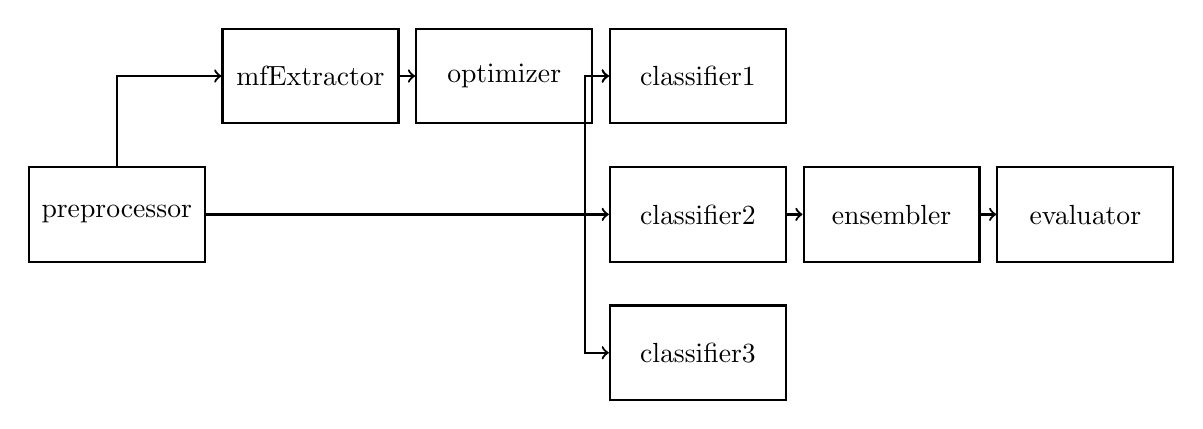
\begin{tikzpicture}	[database/.style={
		cylinder,
		cylinder uses custom fill,
		cylinder body fill=white!50,
		cylinder end fill=white!50,
		shape border rotate=90,
		aspect=0.5,
		draw
	}]
	\node[block, align = center, text width=2cm, text centered, minimum width = 2 cm] (A) at (0,0) {preprocessor};
	\node[block, align = center, text width=2cm, text centered, minimum width = 2 cm] (B) at ([xshift = 7em, yshift = 5em] A) {mfExtractor};
	\node[block, align = center, text width=2cm, text centered, minimum width = 2 cm] (C) at ([xshift = 7em, yshift = 0em] B) {optimizer};
	\node[block, align = center, text width=2cm, text centered, minimum width = 2 cm] (D) at ([xshift = 7em, yshift = 0em] C) {classifier1};
	\node[block, align = center, text width=2cm, text centered, minimum width = 2 cm] (E) at ([xshift = 0em, yshift = -5em] D) {classifier2};
	\node[block, align = center, text width=2cm, text centered, minimum width = 2 cm] (F) at ([xshift = 0em, yshift = -5em] E) {classifier3};
	\node[block, align = center, text width=2cm, text centered, minimum width = 2 cm] (G) at ([xshift = 7em, yshift = 0em] E) {ensembler};
	\node[block, align = center, text width=2cm, text centered, minimum width = 2 cm] (H) at ([xshift = 7em, yshift = 0em] G) {evaluator};
	\draw[->, thick] (A) |- (B);
	\draw[->, thick] (B) to (C);
	\draw[->, thick] (C) to (D);
	\draw[->, thick] (E) to (G);
	\draw[->, thick] (G) to (H);
	\draw[->, thick] (A) to (E);
	\draw[->, thick] (A) -| ([xshift=-0.3cm]E.west) |- (D.west) ;
	\draw[->, thick] (A) -| ([xshift=-0.3cm]E.west) |- (F.west) ;
	\end{tikzpicture}
	\caption[Το υποσύστημα πειράματος]{Το υποσύστημα πειράματος: Δεδομένου ενός σετ δεδομένων δυαδικής ταξινόμησης στην είσοδο το υποσύστημα αυτό εφαρμόζει την κατάλληλη προ-επεξεργασία και στη συνέχεια εξάγει τα μετα-χαρακτηριστικά, ώστε το πακέτο optimizer να προβλέψει τις βέλτιστες υπερ-παραμέτρους με τη βοήθεια των HPP μοντέλων. Στη συνέχεια εκπαιδεύεται ένα πλήθος μοντέλων για κάθε αλγόριθμο μάθησης και το πακέτο ensembler αναλαμβάνει το σχηματισμό του τελικού ensemble. Τελευταίο στάδιο αποτελεί η αξιολόγηση του πειράματος. }
\end{figure}

Τα πακέτα που υλοποιούν τη πλήρη διαδικασία της μηχανικής μάθησης για ένα σετ δεδομένων είναι:
\begin{itemize}
	\item preprocessor. Περιέχει τεχνικές προ-επεξεργασίας όπως καθαρισμού δεδομένων (αντιμετώπιση άγνωστων και άπειρων τιμών), κανονικοποίησης (z-score και min-max), μετασχηματισμού χαρακτηριστικών (PCA, μετασχηματισμός Box-Cox).
	\item mfExtractor. Πρόκειται για το ίδιο πακέτο με αυτό που περιγράφηκε στο υποσύστημα εκπαίδευσης.
	\item optimizer. Στην προκειμένη το πακέτο αυτό αναλαμβάνει την πρόβλεψη των υπερ-παραμέτρων κάθε αλγορίθμου μάθησης χρησιμοποιώντας τα ήδη εκπαιδευμένα HPP μοντέλα.    
	\item classifier$_i$. Κάθε classifier αντιστοιχεί σε ένα μοντέλο με μοναδικό συνδυασμό υπερ-παραμέτρων και αλγορίθμου μάθησης.
	\item ensembler. Το πακέτο αυτό σχηματίζει τον τελικό ensemble από τα διαθέσιμα μοντέλα με την τεχνική του model selection.
	\item evaluator. Υπεύθυνο για την αξιολόγηση του τελικού ensemble με χρήση τεχνικών που είδαμε στην ενότητα \ref{section:eval} και τη σύγκριση της μεθόδου μας με άλλες μεθόδους αναφοράς, οι οποίες αναλύονται στην ενότητα \ref{section:eval_system} με χρήση στατιστικών τεστ.
\end{itemize}
\chapter{Πειραματικά αποτελέσματα}
\section{Περιγραφή πειραμάτων}
Στόχος της παρούσας ενότητας είναι ο έλεγχος του συστήματος Automated Data Scientist, καθώς και της συνεισφοράς των τεχνικών που εφαρμόσαμε και περιγράψαμε στην ενότητα \ref{sec:techniques}. Προς αυτό το σκοπό σχεδιάσαμε τα ακόλουθα πειράματα, τα οποία θα αναλύσουμε στη συνέχεια:
\begin{itemize}
	\item αξιολόγηση των HPP μοντέλων
	\item αξιολόγηση του ensemble με προς-τα-εμπρός επιλογή μοντέλων
	\item συνολική αξιολόγηση του συστήματος
\end{itemize}

\paragraph{Περιγραφή σετ δεδομένων} Για τη διεξαγωγή των πειραμάτων συλλέξαμε ένα πλήθος 123 σετ δεδομένων από διάφορες πηγές. (Στο παράρτημα \ref{appendix:Datasets} βρίσκεται ένας λεπτομερής κατάλογος περιγραφής τους.) Άξονας αναζήτησης κατά τη συλλογή ήταν η εύρεση σετ δεδομένων δυαδικής ταξινόμησης με ετερογενή χαρακτηριστικά, ώστε ο έλεγχος του συστήματος να είναι αντιπροσωπευτικός για το πραγματικό πλήθος σετ δεδομένων. Προκειμένου να υπάρχει μία κοινή διεπαφή για τα πειράματα ήταν απαραίτητος ο "καθαρισμός" των σετ δεδομένων μέσω των ακόλουθων βημάτων:
\begin{itemize}
	\item μετατροπή αρχείων σε comma-delimited .csv. Τα πηγαία αρχεία βρίσκονταν σε μορφές .csv, .txt, .xlsx, .arff και .mysql.
	\item καθορισμός κλάσης. Στη πλειοψηφία των περιπτώσεων η κλάση αναγνωριζόταν χειροκίνητα από την περιγραφή του σετ δεδομένων. Συλλέχθηκαν και σετ δεδομένων που ήταν πολλαπλής ταξινόμησης και παλινδρόμησης. Στην πρώτη περίπτωση έγινε αντιστοίχηση σε δύο ουσιώδεις κλάσεις, ενώ στη δεύτερη βρέθηκε η μέση τιμή της μεταβλητής κλάσης και χρησιμοποιήθηκε ως κατώφλι για το διαχωρισμό των παραδειγμάτων σε δύο κλάσεις.
	\item αναγνώριση άγνωστων τιμών. Στα αρχεία που περιείχαν άγνωστες τιμές χρησιμοποιούνταν διάφοροι συμβολισμοί ("?", "*", "") οι οποίοι αντικαταστάθηκαν από κενά, ώστε να αναγνωρίζονται από την R ως NAs (Not Available).  
\end{itemize}
\section{Αξιολόγηση της τεχνικής βελτιστοποίησης υπερ-παραμέτρων με μετα-μάθηση και χρήση διαστημάτων πρόβλεψης}
Όπως είδαμε στην ενότητα \ref{sec:HPP} προϊόντα αυτής της τεχνικής είναι τα \gls{HPP} μοντέλα, καθένα εκ των οποίων έχει εκπαιδευτεί στη πρόβλεψη μίας υπερ-παραμέτρου ενός αλγορίθμου μηχανικής μάθησης. Σε αυτό το σημείο θα αξιολογήσουμε τα μοντέλα αυτά ως προς το σκοπό τους, δηλαδή πόσο καλά προβλέπουν τις βελτιστοποιημένες υπερ-παραμέτρους. Επίσης, θα σχολιάσουμε τη συνεισφορά της χρήσης διαστημάτων πρόβλεψης.

Για την παραγωγή των σετ μετα-δεδομένων, τα οποία χρησιμοποιούνται για την εκπαίδευση των HPP μοντέλων, είναι απαραίτητα δύο στάδια:
\begin{itemize}
	\item Εξαγωγή των μετα-χαρακτηριστικών κάθε σετ δεδομένων. Τα  81 μετα-χαρακτηριστικά που χρησιμοποιήσαμε περιγράφονται στον Πίνακα \ref{table:meta} και υπολογίστηκαν με χρήση του πακέτου mf\-Extractor του συστήματός μας. Βασίστηκαν σε εκτεταμένη βιβλιογραφική έρευνα και προσπαθούν να συμπεριλάβουν όλα τα είδη μετα-χαρακτηριστικών που εμφανίζονται σε παρόμοιες εργασίες.Πριν τον υπολογισμό τους έγινε μετατροπή των κατηγορικών χαρακτηριστικών σε μεταβλητές-δείκτες, ώστε να υπάρχει ομοιόμορφη αντιμετώπιση.   
	 \begin{table}[!htb]
	 	\footnotesize
	 	\begin{center}
	 	\caption{Λίστα μετα-χαρακτηριστικών, τα οποία χρησιμοποιήθηκαν για την εκπαίδευση των HPP μοντέλων}
	 	\label{table:meta}
	 		\begin{tabular}{ |l l l | } 
	 			\hline
	 			\multicolumn{3}{|c|}{Μετα-χαρακτηριστικά}    \\
	 			\hline
	 			\textbf{Απλά} & \textbf{Θεωρίας Πληροφορίας} &   \textbf{Στατιστικά Kατηγορικά}  \\
	 			Πλήθος χαρακτηριστικών & Εντροπία Κλάσης  &   Πλήθος επιπέδων \\
	 			Λογάριθμος πλήθους χαρακτηριστικών &    & \\
	 			Πλήθος παραδειγμάτων &  \textbf{Στατιστικά Aριθμητικά} & \textbf{Μετα2-}   \\
	 			Λογάριθμος πλήθους παραδειγμάτων & Άθροισμα & Άθροισμα     \\
	 			Πλήθος χαρακτηριστικών με άγνωστες τιμές & Μέση τιμή & Μέση τιμή  \\
	 			Ποσοστό πλήθους χαρακτηριστικών με άγνωστες τιμές & Τυπική απόκλιση & Τυπική απόκλιση   \\
	 			Πλήθος παραδειγμάτων με άγνωστες τιμές & Ελάχιστη τιμή & Ελάχιστη τιμή    \\
	 			Ποσοστό πλήθους παραδειγμάτων με άγνωστες τιμές & Μέγιστη τιμή & Μέγιστη τιμή   \\
	 			Πλήθος άγνωστων τιμών & Κυρτότητα & Κυρτότητα  \\
	 			Λογάριθμος πλήθους άγνωστων τιμών & Λοξότητα & Λοξότητα \\
	 			Πλήθος αριθμητικών χαρακτηριστικών & Ποσοστό \gls{PC}s για $95\%$ διακύμανση & \\
	 			Πλήθος κατηγορικών χαρακτηριστικών &  Κυρτότητα πρώτης \gls{PC}& \\
	 			Πιθανότητες κλάσης & Λοξότητα πρώτης \gls{PC}& \\
	 			Ελάχιστη πιθανότητα κλάσης & &   \\
                Μέγιστη πιθανότητα κλάσης & &  \\
                Μέση τιμή πιθανοτήτων κλάσης & &  \\
                Τυπική απόκλιση πιθανοτήτων κλάσης &  & \\
                \hline
	 		\end{tabular}    
	 	\end{center}
	 \end{table}
	
	Καθώς το πλήθος των μετα-χαρακτηριστικών είναι δυσανάλογο των διαθέσιμων σετ δεδομένων για εκπαίδευση των \gls{HPP} μοντέλων, θα επιστρατευθούν τεχνικές επιλογής των βέλτιστων. Σε πρώτη φάση αφαιρέσαμε τα γραμμικά συσχετισμένα χαρακτηριστικά, όπως αυτά υπολογίστηκαν στο σετ δεδομένων εκπαίδευσης, οπότε η τελική λίστα προέκυψε:
	 \begin{table}[!htb]
	 	\footnotesize
	 	\begin{center}
	 		\caption{Λίστα μετα-χαρακτηριστικών μετά από εφαρμογή φιλτραρίσματος}
	 		\label{table:meta}
	 		\begin{tabular}{ |l l| } 
	 			\hline
	 		     Άθροισμα αθροισμάτων & Τυπική απόκλιση επιπέδων    \\
	 			Άθροισμα μέγιστων τιμών &  Κυρτότητα επιπέδων  \\
	 			Μέση τιμή τυπικών αποκλίσεων  & Λοξότητα επιπέδων    \\
	 		    Μέση τιμή ελαχίστων τιμών &  Πλήθος χαρακτηριστικών  \\
	 			Μέση τιμή κυρτοτήτων &   Λογάριθμος πλήθους χαρακτηριστικών \\
	 			Μέση τιμή λοξοτήτων &    Πλήθος παραδειγμάτων\\
	 			Τυπική απόκλιση ελαχίστων τιμών & Λογάριθμος πλήθους παραδειγμάτων   \\
	 			Ελάχιστη τιμή μέσων τιμών &  Ποσοστό αγνώστων τιμών  \\
	 			Ελάχιστη τιμή τυπικών αποκλίσεων &  Πλήθος αριθμητικών χαρακτηριστικών  \\
	 			Ελάχιστη τιμή ελαχίστων τιμών &  Πλήθος κατηγορικών χαρακτηριστικών  \\
	 			Ελάχιστη τιμή μεγίστων τιμών &  Μέγιστη πιθανότητα κλάσης    \\
	 			Ελάχιστη τιμή λοξοτήτων & Μέση τιμή πιθανοτήτων κλάσης   \\
	 			Κυρτότητα ελαχίστων τιμών & Ποσοστό \gls{PC} για $95\%$ διακύμανση  \\
	 			Κυρτότητα μεγίστων τιμών & Κυρτότητα πρώτης \gls{PC}   \\
	 			Λοξότητα λοξοτήτων & Λοξότητα \gls{PC}   \\
	 		    Άθροισμα επιπέδων &    \\
	 			\hline
	 		\end{tabular}    
	 	\end{center}
	 \end{table}
	\FloatBarrier
	\item Εύρεση των βέλτιστων υπερ-παραμέτρων για κάθε αλγόριθμο. Προς αυτό το σκοπό χρησιμοποιήθηκε η βιβλιοθήκη HPOlib, την οποία έχουμε περιγράψει στην Eνότητα \ref{section:tools}. Ο αλγόριθμος που επιλέχθηκε ήταν ο Tree Parzen Estimator, καθώς είναι σημαντικά ταχύτερος από τους υπόλοιπους. Από τη πλευρά μας ήταν απαραίτητος ο ορισμός του χώρου αναζήτησης υπερ-παραμέτρων και της συνάρτησης κόστους για κάθε αλγόριθμο, η οποία ορίστηκε ως $ Cost = 1- Accuracy$. Στον Πίνακα \ref{table:algorithms} μπορούμε να δούμε τους αλγορίθμους μάθησης με τους οποίους ασχοληθήκαμε, καθώς και τις υπερ-παραμέτρους τους.

\end{itemize}
	\begin{table}[!htb]
		\begin{center}
				\caption[Οι αλγόριθμοι που χρησιμοποιεί το σύστημα Automated Data Scientist και οι υπερ-παράμετροί του]{Οι αλγόριθμοι που χρησιμοποιεί το σύστημα Automated Data Scientist και οι υπερ-παράμετροί τους, όπως τις ορίζει το πακέτο caret. knn: κ-κοντινότερος γείτονας, rpart: δέντρο ταξινόμησης και παλινδρόμησης (CART), nnet: \gls{ΤΝΝ}, svmRadial: \gls{SVM} με χρήση γκαουσιανού πυρήνα, nb: Naive Bayes.} \label{table:meta}
			\begin{tabular}{ |c|c|c|c|c| } 
				\hline
				knn & rpart & nnet & svmRadial & nb\\
				\hline
			    k & cp & size& C & fL\\
			     &  & decay& sigma & usekernel \\
			     &  &    & & adjust \\
				\hline
			\end{tabular}    
		\end{center}
		\label{table:algorithms}
	\end{table} 
	
Στα πειράματα που ακολουθούν έχουμε χρησιμοποιήσει τη τεχνική Leave one out για την αξιολόγηση των μοντέλων, 10-fold cross-validation για τη ρύθμιση και ως κριτήριο της απόδοσης των μοντέλων παλινδρόμησης τη ρίζα του μέσου τετραγωνικού σφάλματος (root mean squared error).

Όσο αφορά τις τεχνικές προ-επεξεργασίας που χρησιμοποιήθηκαν: ως μέθοδο φιλτραρίσματος για επιλογή χαρακτηριστικών ορίζουμε την επιλογή των λιγότερο συσχετισμένων χαρακτηριστικών με βάση τη γραμμική συσχέτιση. Η προς-τα-εμπρός επιλογή χαρακτηριστικών γίνεται με χρήση του πακέτου Boruta~\footnote{https://cran.r-project.org/web/packages/Boruta/Boruta.pdf} και της συνάρτησης rfe του πακέτου caret. Τέλος, ο υπολογισμός των διαστημάτων πρόβλεψης γίνεται με τη βοήθεια των πακέτων kernlab~\footnote{https://cran.r-project.org/web/packages/kernlab/kernlab.pdf} στην περίπτωση του αλγορίθμου \gls{SVM} και του RFinfer~\footnote{https://cran.r-project.org/web/packages/RFinfer/RFinfer.pdf} για χρήση με μοντέλα randomForest.
 
\subsection{Πρόβλεψη υπερ-παραμέτρου πλήθους γειτόνων για αλγόριθμο κ-κοντι\-νότερου γείτονα}

\paragraph{Περιγραφή προβλήματος} Η υπερ-παράμετρος κ στον αλγόριθμο κ-κοντινότερου γείτονα ορίζει πόσα από τα κοντινότερα παραδείγματα θα ληφθούν υπόψιν κατά την πρόβλεψη. Πρόκειται για μία ακέραια και θετική τιμή, το ιστόγραμμα της οποίας, μετά από τη βελτιστοποίησή της στο σετ δεδομένων εκπαίδευσης φαίνεται στο σχήμα  \ref{fig:khist} για βελτιστοποίηση με χρήση του αλγορίθμου \gls{TPE} και στο \ref{fig:kgridhist} για βελτιστοποίηση με πλεγματική αναζήτηση.

\begin{figure}
	\begin{minipage}{0.48\textwidth}
	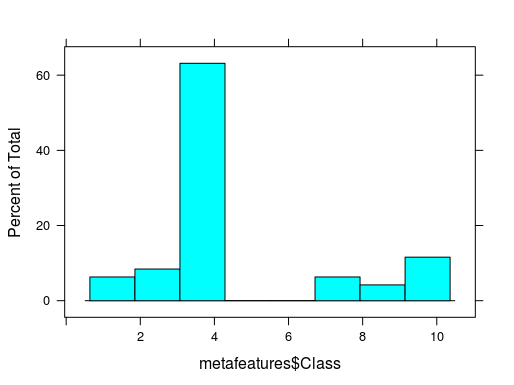
\includegraphics[width=0.9\textwidth]{khist}
	\caption{Ιστόγραμμα υπερ-παραμέτρου κ για βελτιστοποίηση με \gls{TPE}.}	
	\label{fig:khist}
\end{minipage}
	\begin{minipage}{0.48\textwidth}
		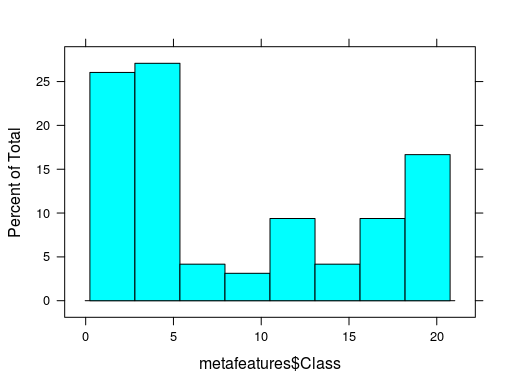
\includegraphics[width=0.9\textwidth]{kgridhist}
		\caption{Ιστόγραμμα υπερ-παραμέτρου κ για βελτιστοποίηση με πλεγματική αναζήτηση.}	
		\label{fig:kgridhist}
	\end{minipage}
\end{figure}

Παρατηρούμε πως στο σχήμα \ref{fig:khist} το δείγμα μας είναι συγκεντρωμένο στην τιμή 4, με αποτέλεσμα οι υπόλοιπες να είναι εξωκείμενες. Καθώς η ιδιότητα αυτή καθιστά την εκπαίδευση του \gls{HPP} μοντέλου ιδιαίτερη αναπτύχθηκε μία νέα τεχνική, αυτή της πρόβλεψης με χρήση General-inflated Generalized Poisson μοντέλου, την οποία αναλύουμε στην επόμενη ενότητα. Επίσης, στην Ενότητα \ref{section:HPPk} θα εκπαιδεύσουμε ένα μοντέλο παλινδρόμησης με χρήση των τιμών που προέκυψαν από την πλεγματική αναζήτηση, θεωρώντας το κ συνεχές. 

\subsubsection{Πρόβλεψη με χρήση General-inflated Generalized Poisson μοντέλου} \label{section:GIGP}
Η στατιστική ανάλυση θετικών και ακεραίων τιμών, οι οποίες στη βιβλιογραφία περιγράφονται ως μεταβλητές πλήθους (count variables) γίνεται με χρήση κατανομών όπως η Poisson και η αρνητική διωνυμική. Καθώς οι κατανομές αυτές περιέχουν ένα μικρό πλήθος παραμέτρων έχει διαπιστωθεί πως δεν είναι επαρκείς για τη περιγραφή της διακύμανσης σε πραγματικά σετ δεδομένων. Τα Γενικευμένα μοντέλα \citep{Neld:Wedd:1972} εισήχθησαν προκειμένου να αντιμετωπιστεί αυτό το πρόβλημα με χρήση βαρών σε μεταβλητές προβλέπτες. Ενώ λοιπόν το μοντέλο Poisson περιγράφεται από τη συνάρτηση μάζας πιθανότητας:

\begin{equation}
 p(\kappa \mid \lambda) = \frac{\lambda^\kappa}{\kappa!} e^{-\lambda}
 \label{eq:poisson}
\end{equation}   

όπου $\kappa$ το ζητούμενο σημείο και $\lambda$ η μέση τιμή της κατανομής, το Γενικευμένο μοντέλο διατυπώνεται ως εξής:

\begin{equation}
 p(\kappa \mid \lambda, \alpha) = \frac{\mu_k}{1+\alpha \mu_k} ^k \frac{1+\alpha k}{k!}^{k-1} e^{\frac{-\mu_k(1+\alpha y_k)}{1+\alpha \mu_k}}
 \label{eq:gpoisson}
\end{equation}

όπου $\mu_k(x_k) = e^{\sum_{}^{} x_{ij} \beta_j}$, με $x_{ij}$ τις τιμές των μεταβλητών προβλεπτών και $\beta$ τα βάρη τους. Η παράμετρος $\alpha$ ρυθμίζει την υπερ-διακύμανση (overdispersion) του μοντέλου.

Η διαπίστωση παρουσίας εκτεταμένους πλήθους μηδενικών τιμών σε πολλά πραγματικά προβλήματα οδήγησε στο σχηματισμό των zero-inflated poisson μοντέλων \citep{Lambert:1992:ZPR:149268.149270}, που προσπαθούν να διορθώσουν την υπερ-διακύμανση υπολογίζοντας ένα μοντέλο για τα μηδενικά και ένα για τις υπόλοιπες τιμές. Ο \citet{gip} γενικεύει τα μοντέλα αυτά διατυπώνοντας τη συνάρτηση πυκνότητας πιθανότητας ενός general-inflated poisson μοντέλου, δηλαδή ενός μοντέλου το οποίο μπορεί να προσαυξηθεί με κατανομές σε οποιοδήποτε σημείο συσσώρευσης τιμών, ως εξής: 
\begin{equation}
 p(\kappa \mid \lambda, \pi_i, 1 \leq i \leq m) = \begin{cases}
 \pi_i + (1-\sum_{i=1}^{m} \pi_i) p(\kappa \mid \lambda) , & \text{εάν $k=k_1, \cdots, k_m$}.\\
 (1-\sum_{i=1}^{m} \pi_i) p(\kappa \mid \lambda), & \text{εάν $k \neq k_i, 1 \leq i \leq m$}.
 \end{cases}
\end{equation}

όπου $p(\kappa \mid \lambda)$ η Poisson συνάρτηση μάζας πιθανότητας όπως αυτή ορίζεται στην Εξίσωση \ref{eq:poisson} και $\pi_i$ μία παράμετρος που ορίζει τη μάζα στο σημείο συσσώρευσης $i$ από τα συνολικά $m$.

Οι \citet{Famoye_onthe} περιγράφουν τα zero-inflated Generalized Poisson μοντέλα, ένα συνδυασμό μεθόδων για την αντιμετώπιση της υπερ-διακύμανσης και του εκτεταμένου πλήθους μηδενικών. 

Για τις ανάγκες του προβλήματος που αντιμετωπίζουμε θα ορίσουμε το General-inflated Genera\-lized Poisson μοντέλο, προκειμένου να εκμεταλλευτούμε τα μετα-χαρακτηριστικά και να αντιμετωπίσουμε την συσσώρευση τιμών στο 4. Προς αυτό το σκοπό θα συνδυάσουμε τα δύο προηγούμενα μοντέλα στην ακόλουθη συνάρτηση μάζας πιθανότητας:

\begin{equation}
 p(\kappa \mid \lambda, \phi_i, 1 \leq i \leq m) = \begin{cases}
 \phi_i + (1-\sum_{i=1}^{m} \phi_i) p(\kappa \mid \lambda, \alpha) , & \text{εάν $k=k_1, \cdots, k_m$}.\\
 (1-\sum_{i=1}^{m} \phi_i) p(\kappa \mid \lambda, \alpha), & \text{εάν $k \neq k_i, 1 \leq i \leq m$}.
 \end{cases}
\end{equation} 
 
 όπου $p(\kappa \mid \lambda, \alpha)$ η Generalized Poisson συνάρτηση μάζας πιθανότητας όπως αυτή ορίζεται στην Εξίσωση \ref{eq:gpoisson} και $\pi_i$ μία παράμετρος που ορίζει τη μάζα στο σημείο συσσώρευσης $i$ από τα συνολικά $m$.
 
 Βασισμένοι στα πειράματα των \citep{gip} και \citep{Famoye_onthe} ακολουθήσαμε την ακόλουθη διαδικασία για την προσαρμογή ενός General-inflated Generalized Poisson μοντέλου στα δεδομένα μας:
 \begin{itemize}
 	\item Προσαρμογή ενός Generalized Poisson μοντέλου για την εύρεση αρχικών τιμών για $\alpha$, $\beta$.
 	\item Προσαρμογή ενός General-inflated Poisson μοντέλου για την εύρεση των αρχικών τιμών των $\pi$.
 	\item Χρήση των αρχικών τιμών για προσαρμογή ενός General-inflated Generalized Poisson μοντέλου.
 \end{itemize}
 
 Η προσαρμογή των μοντέλων γίνεται βελτιστοποιώντας τις παραμέτρους με χρήση της τεχνικής Maximum Likelihood Estimation με αλγόριθμο αναζήτησης τη μέθοδο Nelder-Mead. Καθώς ο αλγόριθμος αυτός είναι ευαίσθητος στις αρχικές τιμές των παραμέτρων πραγματοποιήσαμε cross-validation σε ένα πλέγμα αρχικών τιμών για τα βήματα 1 και 2. Στα διάγραμματα \ref{fig:low} και \ref{fig:high} βλέπουμε τη συνάρτηση μάζας πιθανότητας του προσαρμοσμένου μοντέλου και τις πραγματικές συχνότητες των δεδομένων μας:
 
\begin{figure}[!htb]
	\begin{minipage}{0.48\textwidth}
		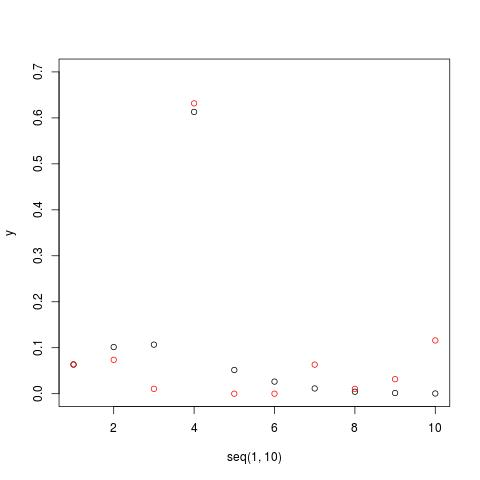
\includegraphics[width=0.9\textwidth]{gigp_low}
		\caption{Σύγκριση General-inflated Generalized Poisson συνάρτηση μάζας πιθανότητες με πραγματικές συχνότητες: Αρχικοποίηση που προσαρμόζεται καλά στο σημείο συσσώρευσης και στις χαμηλές τιμές.}	
		\label{fig:low}
	\end{minipage}
	\begin{minipage}{0.48\textwidth}
		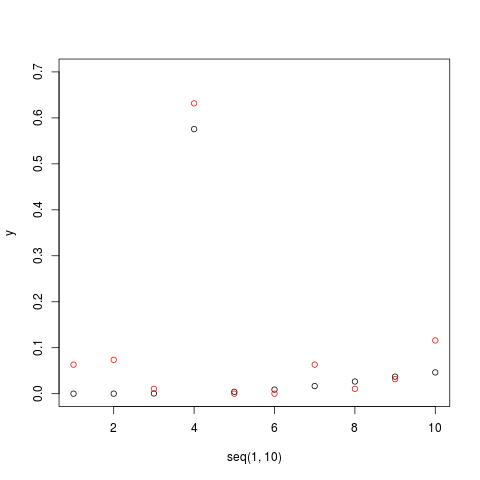
\includegraphics[width=0.9\textwidth]{gigp_high}
		\caption{Σύγκριση General-inflated Generalized Poisson συνάρτηση μάζας πιθανότητες με πραγματικές συχνότητες: Αρχικοποίηση που προσαρμόζεται καλά στο σημείο συσσώρευσης και στις υψηλές τιμές.}	
		\label{fig:high}
	\end{minipage}
\end{figure}
\FloatBarrier
\subsubsection{Εκπαίδευση μοντέλου παλινδρόμησης για κ του κ-κοντινότερου γείτονα} \label{section:HPPk}
\begin{figure}[!htb]
	\footnotesize
	\begin{center}
		\captionof{table}{Επιλογή αλγορίθμου για την υπερ-παράμετρο k του κ-κοντινότερου γείτονα}
		\begin{tabular}{ |c|c|c|c| } 
			\hline
			& Χωρίς προ-επεξεργασία & Με επιλογή χαρακτηριστικών & \pbox{20cm}{Με επιλογή χαρακτηριστικών\\ και κανονικοποίηση} \\
			\hline
			lm &  & $14 \cdot e+15$ &   \\
			\hline
			lm + log & & $7.946205 ^{*}$~\footnote{Η συνοδεία μιας μέτρησης με $^*$ υποδηλώνει ότι κρίθηκε χρήσιμο να αφαιρεθούν κάποια παραδείγματα από το σετ ελέγχου, καθώς την επηρέαζαν υπερβολικά. Αποτελεί ικανότητα του συστήματος η αναγνώριση τέτοιων παραδειγμάτων και η αποδοχή αδυναμίας εκπαίδευσης για αυτά. }& \\
			\hline
			svmRadial & $7.387213$ &$5.813214$& \\
			\hline
			svmRadial + log& $6.255705$ & $5.89$& $6.096127$\\
			\hline
			ranger + log  & $5.794678$ & 5.39141 & $5.227026$\\
			\hline
		\end{tabular}   
	\end{center}
\end{figure}

Στη συνέχεια εκπαιδεύουμε ένα μοντέλο παλινδρόμησης με χρήση του αλγορίθμου randomForest με λογαριθμικό μετασχηματισμό και εφαρμογή φιλτραρίσματος, προς-τα-εμπρός επιλογής χαρακτηριστικών και κανονικοποίησης κατά την προ-επεξεργασία.

\begin{figure}[!htb]
	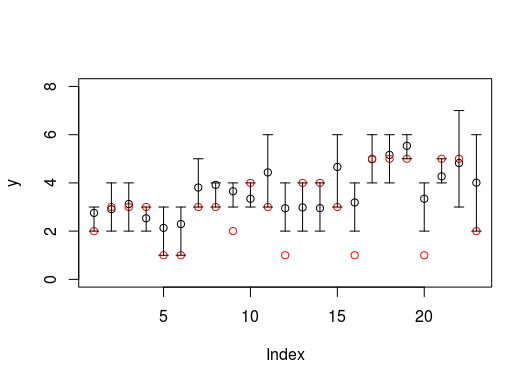
\includegraphics[width=0.9\textwidth]{test_intervals_k}
		\caption[Διάγραμμα διαστημάτων πρόβλεψης για υπερ-παράμετρο decay]{Διάγραμμα διαστημάτων πρόβλεψης για υπερ-παράμετρο k.}	
	\label{fig:high} 
\end{figure}
\FloatBarrier
\subsection{Πρόβλεψη υπερ-παραμέτρου πολυπλοκότητας για αλγόριθμo δέντρου ταξινόμησης} 
\begin{figure}[!htb]
	\footnotesize
	\begin{center}
		\captionof{table}{Επιλογή αλγορίθμου για την υπερ-παράμετρο cp του δέντρου ταξινόμησης}
		\begin{tabular}{ |c|c|c| } 
			\hline
			 & Με κανονικοποίηση & \pbox{20cm}{Με επιλογή χαρακτηριστικών\\ και κανονικοποίηση} \\
			 \hline
			lm & & $1.542080$  \\
			\hline
			lm + log && $0.78553$\\
			\hline
			svmRadial && $0.9514741$\\
			\hline
			svmRadial + log& $0.767217$& $0.768084$\\
			\hline
			ranger + log  &$0.755421$&$0.692675$\\
			\hline
			rpart + log &&$0.8007$\\
			\hline
			blackboost + log && $0.800744$ \\
			\hline
			nnet + log  && $1.3621$\\
			\hline
			cubist + log && $0.692675$ \\
			\hline
			xgbTree + log && $1.204$\\
			\hline
		\end{tabular}   
	\end{center}
\end{figure}

Στη συνέχεια εκπαιδεύουμε ένα μοντέλο παλινδρόμησης με χρήση του αλγορίθμου randomForest με λογαριθμικό μετασχηματισμό και εφαρμογή φιλτραρίσματος, προς-τα-εμπρός επιλογής χαρακτηριστικών και κανονικοποίησης κατά την προ-επεξεργασία.

\begin{figure}[!htb]
	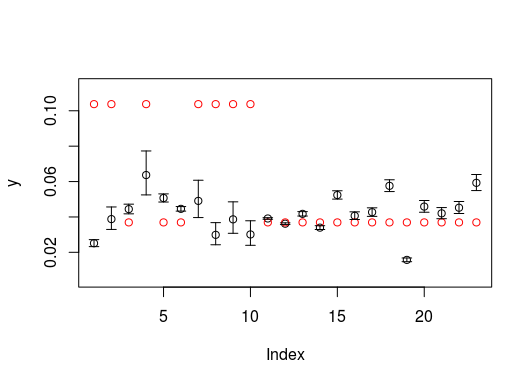
\includegraphics[width=0.9\textwidth]{test_intervals_cp}
			\caption[Διάγραμμα διαστημάτων πρόβλεψης για υπερ-παράμετρο decay]{Διάγραμμα διαστημάτων πρόβλεψης για υπερ-παράμετρο cp.}
	\label{fig:high} 
\end{figure}
\FloatBarrier
\subsection{Πρόβλεψη υπερ-παραμέτρου πλάτους πυρήνα για τον αλγόριθμο \gls{SVM}} 
\begin{figure}[!htb]
	\footnotesize
				\begin{center}
		\captionof{table}{Επιλογή αλγορίθμου για την υπερ-παράμετρο cp του δέντρου ταξινόμησης}
				\resizebox{\textwidth}{!}{ 
		\begin{tabular}{ |c|c|c|c|c|c|c| } 
			\hline
			& \pbox{20cm}{Χωρίς\\ προ-επεξεργασία} & \pbox{20cm}{Με αφαίρεση\\ ακραίων τιμών} & \pbox{20cm}{Με προς-τα-εμπρός\\ επιλογή χαρακτηριστικών} & Με φιλτράρισμα χαρακτηριστικών & \pbox{20cm}{Με φιλτράρισμα χαρακτηριστικών\\ και αφαίρεση ακραίων τιμών} &\pbox{20cm}{Με φιλτράρισμα χαρακτηριστικών\\ και αφαίρεση ακραίων τιμών\\ και κανονικοποίηση}  \\
			\hline
			lm & $15 \cdot e+13$ & $6.296997 ^*$ & $7 \cdot e+9$& $10 \cdot e+10 $ &  $69993$& $3.076596^*$     \\
			\hline
			lm + log & $4.2 \cdot e+10 ^*$ &  $4.239327$&$2.563388^*$ & Inf & $4.055437 ^*$&  $3.423858^*$\\
			\hline
			svmRadial & $2.682720$& $2.609875$ & $2.685054$ & $2.588112$ & &  $2.585245$  \\
			\hline
			svmRadial + log & $2.7075885$ & $2.702844$ & & $2.720634$ & $2.664860$ & $2.690744$   \\
			\hline
			ranger & & & & & $2.576414$& $2.671640$ \\
			\hline
			ranger + log  & &  $2.453491$ & $2.679798$& $2.6248730$& $2.696213$ & $2.530286$\\
			\hline
		\end{tabular}  }
	\end{center}
\end{figure}

Στη συνέχεια εκπαιδεύουμε ένα μοντέλο παλινδρόμησης με χρήση του αλγορίθμου randomForest με λογαριθμικό μετασχηματισμό και εφαρμογή αφαίρεσης ακραίων τιμών, φιλτραρίσματος, προς-τα-εμπρός επιλογής χαρακτηριστικών κανονικοποίησης κατά την προ-επεξεργασία.
\begin{figure}[!htb]
	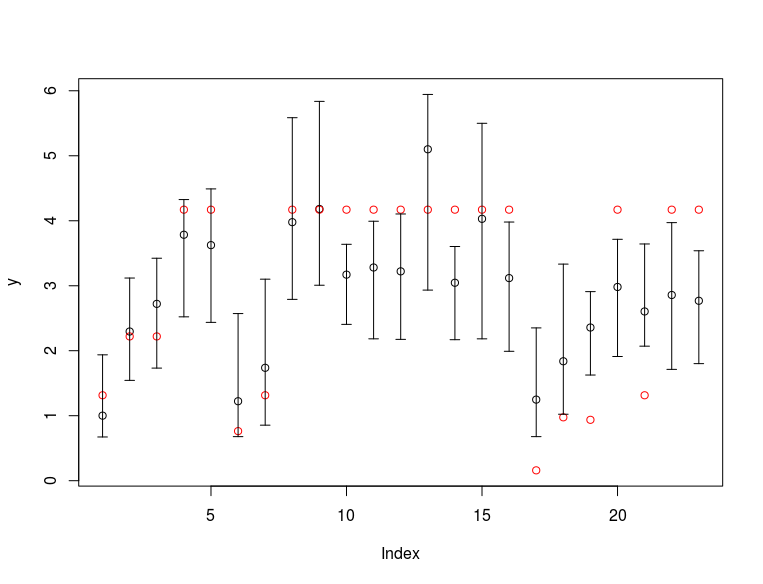
\includegraphics[width=0.9\textwidth]{test_intervals_sigma}
			\caption[Διάγραμμα διαστημάτων πρόβλεψης για υπερ-παράμετρο decay]{Διάγραμμα διαστημάτων πρόβλεψης για υπερ-παράμετρο sigma.}
	\label{fig:high} 
\end{figure}
\FloatBarrier
\subsection{Πρόβλεψη υπερ-παραμέτρου κόστους για τον αλγόριθμo \gls{SVM} }
\begin{figure}[!htb]
	\footnotesize
	\begin{center}
		\captionof{table}{Επιλογή αλγορίθμου για την υπερ-παράμετρο C του \gls{SVM}}
		\begin{tabular}{ |c|c|c|c| } 
			\hline
			& Με κανονικοποίηση & Με επιλογή χαρακτηριστικών & \pbox{20cm}{Με επιλογή χαρακτηριστικών\\ και κανονικοποίηση} \\
			\hline
			lm & $12.91$  & $12.8225$ & $12.82250$  \\
			\hline
			lm + log & $15.618852^*$ & $9.991954 ^{*}$& $9.991954^*$ \\
			\hline
			svmRadial & $10.401787$ &$10.507888$& $10.21597$\\
			\hline
			svmRadial + log& $11.136914$ & $10.676247$& $10.840548$\\
			\hline
			ranger + log  & $9.997852$ & $9.319905$ & $9.294558$\\
			\hline
		\end{tabular}   
	\end{center}
\end{figure}

Στη συνέχεια εκπαιδεύουμε ένα μοντέλο παλινδρόμησης με χρήση του αλγορίθμου randomForest με λογαριθμικό μετασχηματισμό και εφαρμογή φιλτραρίσματος, προς-τα-εμπρός επιλογής χαρακτηριστικών και κανονικοποίησης κατά την προ-επεξεργασία.

\begin{figure} [!htb]
	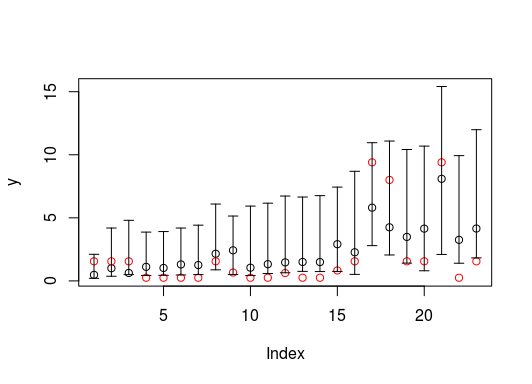
\includegraphics[width=0.9\textwidth]{test_intervals_C}
		\caption[Διάγραμμα διαστημάτων πρόβλεψης για υπερ-παράμετρο decay]{Διάγραμμα διαστημάτων πρόβλεψης για υπερ-παράμετρο C.}
	\label{fig:high} 
\end{figure}
\FloatBarrier
\subsection{Πρόβλεψη υπερ-παραμέτρου μεγέθους για τον αλγόριθμo \gls{ΤΝΝ}}
\begin{figure}[!htb]
	\footnotesize
	\begin{center}
		\captionof{table}{Επιλογή αλγορίθμου για την υπερ-παράμετρο size του \gls{ΤΝΝ}}
		\resizebox{\textwidth}{!}{ 
			\begin{tabular}{ |c|c|c|c|c|c| } 
				\hline
				& \pbox{20cm}{Χωρίς\\ προ-επεξεργασία} & \pbox{20cm}{Με αφαίρεση\\ ακραίων τιμών\\ και κανονικοποίηση} & \pbox{20cm}{Με φιλτράρισμα, \\προς τα εμπρός επιλογή χαρακτηριστικών (Boruta)\\ και αφαίρεση ακραίων τιμών} & \pbox{20cm}{Με φιλτράρισμα, \\προς τα εμπρός επιλογή χαρακτηριστικών (Boruta)\\, αφαίρεση ακραίων τιμών\\ και κανονικοποίηση} & \pbox{20cm}{Με φιλτράρισμα, \\προς τα εμπρός επιλογή χαρακτηριστικών (rfe),\\ κανονικοποίηση και αφαίρεση ακραίων τιμών} \\
			\hline
			lm + log & $4.8964 ^*$ & $4.042651$ & $2.534214$ & $2.534214$&  \\
			\hline
			svmRadial & $2.354932$& $2.358656$ & $2.164228$ & $2.113806$ & 2.208724  \\
			\hline
			svmRadial + log & $2.344243$ & $2.320754$ & $2.113830$& $2.045345$ &  2.180961  \\
			\hline
			ranger & & & $2.131324$& $2.115296$ &  \\
			\hline
			ranger + log  & $2.286583$ & $2.339490$  & $2.367264$ & $2.135809$ & \\
			\hline
			glm  &  &   &   $2.367264$ & $2.367264$ & \\
			\hline
			glm + log  &  &   &   $2.534214$ & $2.53421417$ & \\
			\hline    				
			\end{tabular}  }
		\end{center}
	\end{figure}
	
Στη συνέχεια εκπαιδεύουμε ένα μοντέλο παλινδρόμησης με χρήση του αλγορίθμου svmRadial με λογαριθμικό μετασχηματισμό και εφαρμογή αφαίρεσης ακραίων τιμών, φιλτραρίσματος, προς-τα-εμπρός επιλογής χαρακτηριστικών και κανονικοποίησης κατά την προ-επεξεργασία.
\begin{figure}[!htb]
	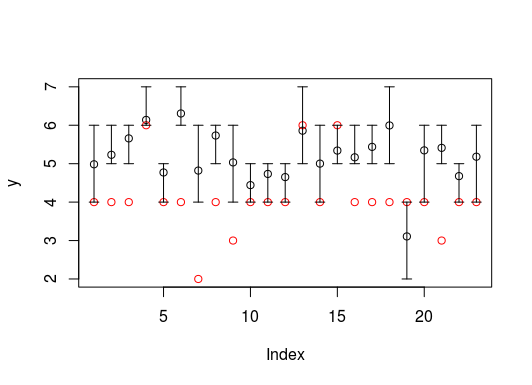
\includegraphics[width=0.9\textwidth]{test_intervals_size}
		\caption[Διάγραμμα διαστημάτων πρόβλεψης για υπερ-παράμετρο decay]{Διάγραμμα διαστημάτων πρόβλεψης για υπερ-παράμετρο size.}
	\label{fig:high} 
\end{figure}
\FloatBarrier
\subsection{Πρόβλεψη υπερ-παραμέτρου φθοράς για τον αλγόριθμo \gls{ΤΝΝ}} 
\begin{figure}[!htb]
	\footnotesize
	\begin{center}
		\captionof{table}{Επιλογή αλγορίθμου για την υπερ-παράμετρο decay του \gls{ΤΝΝ}}
		\resizebox{\textwidth}{!}{ 
			\begin{tabular}{ |c|c|c|c|c|c| } 
				\hline
				& \pbox{20cm}{Με αφαίρεση\\ ακραίων τιμών} & \pbox{20cm}{Με αφαίρεση\\ ακραίων τιμών\\κανονικοποίηση} & \pbox{20cm}{Με φιλτράρισμα, \\προς τα εμπρός επιλογή χαρακτηριστικών (Boruta)\\ και αφαίρεση ακραίων τιμών} & \pbox{20cm}{Με φιλτράρισμα, \\προς τα εμπρός επιλογή χαρακτηριστικών (Boruta)\\, αφαίρεση ακραίων τιμών\\ και κανονικοποίηση} & \pbox{20cm}{Με φιλτράρισμα, \\προς τα εμπρός επιλογή χαρακτηριστικών (rfe),\\ κανονικοποίηση και αφαίρεση ακραίων τιμών} \\
				\hline
				lm  & $1.3346 ^*$ & 1.340122  & 0.2674278  & 0.267428 &  \\
				\hline
				lm + log & $2.08406 ^*$ & 2.084079 & 0.277538& 0.277538&  \\
				\hline
				svmRadial & 0.279624 & 0.279403  & 0.270774 & 0.268606  & 0.267425   \\
				\hline
				svmRadial + log & 0.252120  & 0.253401 & 0.251316 & 0.252016  & 0.255515   \\
				\hline
				ranger & 0.276386 & 0.285601 & 0.244 & 0.247057  &  \\
				\hline
				ranger + log  & 0.250204 &  0.248379 & 0.24289  & 0.240159  & \\
				\hline    				
			\end{tabular}  }
		\end{center}
	\end{figure}
	
Στη συνέχεια εκπαιδεύουμε ένα μοντέλο παλινδρόμησης με χρήση του αλγορίθμου randomforest με λογαριθμικό μετασχηματισμό και εφαρμογή αφαίρεσης ακραίων τιμών, φιλτραρίσματος, προς-τα-εμπρός επιλογής χαρακτηριστικών και κανονικοποίησης κατά την προ-επεξεργασία.

\begin{figure}[!htb]
	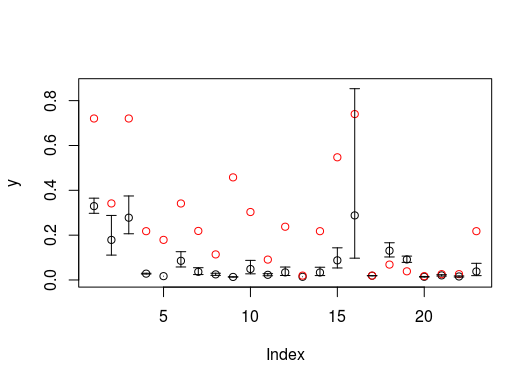
\includegraphics[width=0.9\textwidth]{test_intervals_decay}
	\caption[Διάγραμμα διαστημάτων πρόβλεψης για υπερ-παράμετρο decay]{Διάγραμμα διαστημάτων πρόβλεψης για υπερ-παράμετρο decay.}	
	\label{fig:high} 
\end{figure}
\FloatBarrier

\paragraph{Συμπεράσματα}
Τα μοντέλα HPP που εκπαιδεύσαμε απέχουν κατά πολύ από το να προβλέπουν επακριβώς τις υπερ-παραμέτρους. Το γεγονός αυτό μάλλον οφείλεται στα μετα-χαρακτη\-ρι\-στικά και συγκεκριμένα την αδυναμία τους να περιγράψουν τις συναρτήσεις-στόχους που θέσαμε. Είναι γεγονός πως δεν είμαστε βέβαιοι για την επιτευξιμότητα της πρόβλεψης υπερ-παραμέτρων, τα πειράματά μας ωστόσο δεν απορρίπτουν την ύπαρξη κάποια συσχέτισης μεταξύ αυτών και των μετα-χαρακτηριστικών.

Η προσθήκη των διαστημάτων πρόβλεψης αποδεικνύεται ότι αναιρεί την αδυναμία των μοντέλων HPP, καθώς η βέλτιστη τιμή βρίσκεται σχεδόν πάντα μέσα στο διάστημα πρόβλεψης, προσδίδοντας βαρύτητα στην αξιολόγηση του ensemble, η οποία ακολουθεί.  
\section{Αξιολόγηση της τεχνικής σχηματισμού ensemble με προς τα εμπρός επιλογή μοντέλων} \label{section:tensemble}
H αξιολόγηση της τεχνικής ensemble που χρησιμοποιήσαμε επιχειρεί να επιβεβαιώσει δύο προσδοκίες:
\begin{itemize}
	\item Ο ensemble παρουσιάζει τουλάχιστον το ίδιο καλή απόδοση με το καλύτερο μοντέλο, το οποίο βρίσκεται στην αποθήκη βελτιστοποιημένων μοντέλων. Προς αυτό το σκοπό θα συγκρίνουμε την απόδοση του ensemble με αυτήν του εκάστοτε βέλτιστου μοντέλου με δύο τεχνικές: στατιστικά τεστ υπόθεσης και διαγράμματα προφίλ απόδοσης.
	\item Ο ensemble προσθέτει μοντέλα με το βέλτιστο τρόπο. Ουσιαστικά θέλουμε να επιβεβαιώσουμε τη σωστή λειτουργία του ensemble, δηλαδή ότι σε κάθε επανάληψη έχουμε είτε σταθερή είτε βελτιωμένη απόδοση.
\end{itemize}

Για τα πειράματά μας εκπαιδεύουμε τα μοντέλα στο $80\%$ των σετ δεδομένων και κρατάμε τα υπόλοιπα για την αξιολόγηση του ensemble, η οποία γίνεται ως εξής: εξάγονται τα μετα-χαρακτηριστικά των σετ δεδομένων, προβλέπονται οι βέλτιστες υπερ-παράμετροι για κάθε αλγόριθμο μάθησης, εκπαιδεύονται τα μοντέλα και τέλος σχηματίζεται ο ensemble. Για κάθε σετ δεδομένων καταγράφεται η απόδοση του ensemble και του βέλτιστου μοντέλου ως η ακρίβεια (accuracy) που επιτεύχθηκε με 10-fold cross-validation. 

Εφαρμόζωντας το Wilcoxon-rank sum τεστ με επίπεδο εμπιστοσύνης $95\%$ διαπιστώνουμε πως ..., καθώς το p-value ισούται με ... .

\paragraph{Διαγράμματα προφίλ απόδοσης} 	Τα διαγράμματα προφίλ απόδοσης (performance profile plots) \citep{Dolan2002} αποτελούν ένα εργαλείο αξιολόγησης και σύγκρισης της απόδοσης εργαλείων βελτιστοποίησης. Χρησιμοποιούνται σε περιπτώσεις εφαρμογής διαφορετικών τεχνικών βελτιστοποίησης σε ένα σύνολο προβλημάτων ως εναλλακτική απεικόνιση εκτενών πινάκων, μιας συνηθισμένης και προβληματικής λύσης. Το προφίλ απόδοσης είναι η αθροιστική συνάρτηση κατανομής μιας τεχνικής για μία μετρική απόδοσης.

Ως μετρική απόδοσης ορίζουμε το λόγο της απόδοσης της τρέχουσας τεχνικής προς τη μεγαλύτερη απόδοση που επιτεύχθηκε από οποιαδήποτε τεχνική για ένα συγκεκριμένο σετ δεδομένων, δηλαδή

\begin{equation}
r_{p,s}= \frac{t_{p,s}}{\max\{{t_{p,s} : s \in S}\}}    
\end{equation} 

όπου r ο λόγος απόδοσης, t η ακρίβεια, p το σετ δεδομένων και s η τεχνική.

Το διάγραμμα απεικονίζει τη τιμή
\begin{equation}
\rho_{\tau}= \frac{size\{{p \in P : r_{p,s} \leq \tau  }\}}{n_p}   
\end{equation}

όπου $n_p$ το πλήθος των σετ δεδομένων. Η τιμή αυτή εκφράζει την πιθανότητα μία τεχνική να βρίσκεται σε απόσταση $\tau$ από τον καλύτερο λόγο απόδοσης.  Επομένως το σημείο $\tau = 1$ εκφράζει τη πιθανότητα μία τεχνική να είναι η βέλτιστη.


\begin{figure}[!htb]
	\begin{center}
		\caption[Διάγραμμα προφίλ απόδοσης για τη σύγκριση του ensemble με το βέλτιστο μοντέλο]{Διάγραμμα προφίλ απόδοσης για τη σύγκριση του ensemble με το βέλτιστο μοντέλο: Παρατηρούμε πως }
	\end{center}
\end{figure}

\begin{figure}[!htb]
	\begin{center}
		\caption[Διάγραμμα εξέλιξης ensemble για το σετ δεδομένων (όνομα)]{Διάγραμμα εξέλιξης ensemble για το σετ δεδομένων (όνομα): Παρατηρούμε πως σε κάθε επανάληψη η απόδοση του ensemble είτε μειώνεται είτε παραμένει σταθερή. }
	\end{center}
\end{figure} 	

\paragraph{Συμπεράσματα}
\section{Αξιολόγηση συστήματος Automated Data Scientist}\label{section:eval_system}
Η αξιολόγηση του Automated Data Scientist στοχεύει να αποδείξει ότι το σύστημα που έχουμε σχεδιάσει έχει απόδοση συγκρίσιμη με τεχνικές της σύγχρονης βιβλιογραφίας. Καθώς η ουσιαστική πρωτοτυπία του συστήματος βρίσκεται στον τρόπο με τον οποίο γίνεται η βελτιστοποίηση των υπερ-παρα\-μέ\-τρων για τα μοντέλα μηχανικής μάθησης που χρησιμοποιούμε θα συγκρίνουμε το σύστημά μας με δύο τεχνικές βελτιστοποίησης:
\begin{itemize}
	\item πλεγματική αναζήτηση. Πρόκειται για τη συνηθέστερη τεχνική αναζήτησης υπερ\-παραμέτρων μέχρι και σήμερα.
	\item Tree Parzen Estimator. Η τεχνική αυτή, που έχει περιγραφεί στην ενότητα \ref{section:SMBO} αποτελεί state of the art στο χώρο του AutoML.
\end{itemize}

Η διεξαγωγή των πειραμάτων ακολουθεί τη λογική της ενότητας \ref{section:tensemble}. Έχουμε πραγματοποιήσει 6 διαφορετικά πειράματα: ένα για το συνολικό σύστημα και ένα χρησιμοποιώντας στον ensemble μοντέλα μόνο ενός αλγορίθμου μάθησης. Οι υποπεριπτώσεις αυτές λαμβάνονται υπόψη για τη σύγκριση των τριών τεχνικών επί ίσοις όροις. Φυσικά εμείς ενδιαφερόμαστε περισσότερο για την απόδειξη υπεροχής του συνολικού συστήματος.  

[Ακολουθούν τα διαγράμματα προφίλ απόδοσης]
	
\paragraph{Συμπεράσματα}
\chapter{Βιβλιογραφία}
Η βιβλιογραφία αντικατοπτρίζει την προσπάθεια της κοινότητας να αυτοματοποιήσει τη διαδικασία της μηχανικής μάθησης προσφέροντας πακέτα λογισμικού που την υλοποιούν και έρευνες που επιχειρούν να επεκτείνουν την τρέχουσα κατάσταση. Οι εξελίξεις εντοπίζονται σε τομείς όπως η βελτιστοποίηση υπερ-παραμέτρων, η εισαγωγή μετα-μάθησης και η ανάπτυξη καλύτερων τεχνικών σχηματισμού πολύπλοκων μοντέλων.

Η ανατροπή του τοπίου για τη βελτιστοποίηση υπερ-παραμέτρων συνέβη όταν οι \citet{Bergstra:2012:RSH:2188385.2188395} απέδειξαν πως η τεχνική της πλεγματικής αναζήτησης επιφέρει αποτέλεσμα χειρότερο από την τυχαία αναζήτηση. Έκτοτε έχουν δοκιμαστεί γενετικοί αλγόριθμοι \citep{1554741}, αναζήτηση κλίσης \citep{wassenberg} και η bayesian βελτιστοποίηση, η οποία φαίνεται να έχει επικρατήσει με τη μορφή της τεχνικής SMBO \citep{DBLP:journals/corr/abs-1208-3719}. Οι \citet{HutHooLeyMur10} εισάγουν την έννοια των χρονικών ορίων στη διαδικασία της βελτιστοποίησης λαμβάνοντας υπόψιν ως κόστος, τόσο την ποιότητ,α όσο και το χρόνο.

Προσπάθειες εισαγωγής μετα-μάθησης κατέβαλαν οι \citet{Feurer:2014:UMI:3015544.3015549}, οι οποίοι χρησιμοποίησαν μετα-χαρακτηριστικά των σετ δεδομένων, ώστε να προβλέψουν τιμές των υπερ-παραμέτρων που, με βάση παλαιότερα πειράματα, πιθανώς να οδηγούν σε καλύτερα μοντέλα. Ωστόσο η διαπίστωση αδυναμίας ικανοποιητικής πρόβλεψης τους οδήγησε σε χρήση των τιμών αυτών για αρχικοποίηση του SMBO αλγόριθμου αναζήτησης που χρησιμοποιούν.  

Οι \citet{kuba2002exploiting} χρησιμοποιούν δέντρα παλινδρόμησης για να προβλέψουν τις παράμετρους $\epsilon$ και $\sigma$ ενός \gls{SVM}. Έπειτα από μία διεξοδική ανάλυση των μετα-χαρακτηριστικών καταλήγουν σε μη ικανοποιητικά μοντέλα πρόβλεψης, πρόβλημα που προτείνουν να διορθώσουν εισάγοντας ένα τελικό στάδιο τοπικής αναζήτησης γύρω από τις προβλέψεις τους.


Οι \citet{Soares2004} ασχολούνται με τη πρόβλεψη της υπερ-παραμέτρου $\sigma$ ενός SVM, που καθορίζει το πλάτος του γκαουσιανού πυρήνα. Χρησιμοποιώντας μετα-χαρακτηριστι\-κά των σετ δεδομένων και ένα μοντέλο k-κοντινότερου γείτονα προβλέπουν τη διάταξη προκαθορισμένων τιμών της υπερ-παραμέτρου και με τη τεχνική της Top-Ν αξιολόγησης επιλέγουν τις βέλτιστες τιμές. Το σύστημά τους δε προβλέπει άμεσα τη βέλτιστη υπερ-παράμετρο, αλλά κατατάσσει ένα προκαθορισμένο σετ ως προς την απόδοσή του στο νέο σετ δεδομένων. Η μεθοδολογία τους απαιτεί τον προ-υπολογισμό της απόδοσης του SVM στα σετ δεδομένων εκπαίδευσης για τις διαθέσιμες τιμές, προσέγγιση απαγορευτική για πολυδιάστατους αλγορίθμους μάθησης. Επίσης, η ελευθερία επιλογής του Ν αυξάνει την απόδοση, αλλά καθιστά μια σχεδιαστική επιλογή, η οποία μειώνει τον αυτοματισμό της διαδικασίας. Τέλος, η μέθοδός τους εξασφαλίζει χειρότερο αποτέλεσμα από αυτό που επιτυγχάνεται με τη τεχνική cross-validation, ωστόσο κρίνεται ικανοποιητική καθώς επιφέρει χρονική και υπολογιστική βελτίωση. 

Ενδιαφέρον παρουσιάζουν οι προσπάθειες των ερευνητών να αναλύσουν τη διαδικασία της μετα-μάθησης, ώστε να ανακαλύψουν τους μηχανισμούς που τη διέπουν με στόχο την αναγνώριση χρήσιμων χαρακτηριστικών, κατάλληλων αλγορίθμων μετα-μάθησης και γενικότερα την παραγωγή μετα-γνώσης. Οι \citet{Brazdil2009} τοποθετούν τη μετα-μάθηση μέσα στον τομέα της Εξόρυξης Δεδομένων, την προσδιορίζουν ως την ικανότητα προσαρμογής με βάση προϋπάρχουσα εμπειρία, παραθέτουν την ιστορική της εξέλιξη και παρουσιάζουν συστήματα που τη χρησιμοποιούν.

Εκτεταμένη έρευνα πάνω στη χρήση \gls{IBL} αλγορίθμων για πρόβλεψη υπερ-παραμέτρων πραγματοποιούν οι \citet{Abdulrahman:2014:MCA:3015544.3015557}. Αποδίδουν την καταλληλότητα των αλγορίθμων αυτών για μοντέλα μετα-μάθησης στην εκ φύσεως αδυναμία του προβλήματος για δημιουργία γενικών μοντέλων λόγω των περιορισμένων δεδομένων και της ιδιαιτερότητας κάποιων υπερ-παραμέτρων και τη δυνατότητά τους να ενημερώνονται χωρίς εκπαίδευση. Επίσης, παροτρύνουν προς την επιλογή μετα-χαρακτηριστικών με βάση τη σημασιολογική τους συνεισφορά στο πρόβλημα και την αξιολόγησή τους ως προς τη συσχέτισή τους με την υπερ-παράμετρο υπό πρόβλεψη. 

Οι \citet{Reif_meta2-features:} αναγνωρίζουν το πρόβλημα που προκύπτει στη προσπάθεια εφαρμογής μετα-μάθησης όταν τα μετα-χαρακτηριστικά έχουν διαφορετικό πλήθος για τα σετ δεδομένων και εισάγουν την έννοια των μετα-μετα-χαρακτηριστικών. Πρόκειται για μια προσπάθεια στατιστικής περιγραφής των μετα-χαρακτηριστικών μέσω στατιστικών δεικτών όπως η μέση τιμή, η διακύμανση και η κυρτότητα. Η τεχνική τους, πέρα από τη λύση του προηγούμενου προβλήματος, εμπλουτίζει τη πληροφορία που διατίθεται για μετα-μάθηση. Οι \citet{Bensusan:2001:EPA:645328.650030} εισάγουν τη χρήση πληροφορίας προερχόμενης από τα ιστογράμματα των μετα-χαρακτηριστικών προκειμένου να αποτυπώσουν πληρέστερα την κατανομή τους.

Η συνειδητοποίηση ότι η επίλυση προβλημάτων με χρήση αυτοματοποιημένων συστημάτων απαιτεί τη χρήση πληθώρας τεχνικών και αλγορίθμων οδήγησε στην αναζήτηση βελτιστοποιημένων μεθόδων συνδυασμού μοντέλων μάθησης. Οι \citet{Caruana:2004:ESL:1015330.1015432} εισάγουν τη μέθοδο σχηματισμού ensembles μοντέλων με την τεχνική της προς-τα-εμπρός επιλογής αναπτύσσοντας τεχνικές για την εξασφάλιση της καλής ποιότητας και την αποφυγή υπερ-προσαρμογής του τελικού ensemble. Διαφορετική προσέγγιση ακολοθούν οι \citet{ensemble}, οι οποίοι απορρίπτουν το σχηματισμό του ensemble ως τελικό στάδιο. Η προσέγγισή τους ενσωματώνει το σχηματισμό στη διαδικασία της βελτιστοποίησης των υπερ-παραμέτρων καθώς η συνάρτηση κόστους υπό βελτιστοποίηση αφορά τη συνεισφορά ενός μοντέλου στον ensemble και η εισαγωγή ενός νέου μοντέλου στη συλλογή γίνεται με μία round robin στρατηγική. 
\chapter{Σχετική Δουλειά}
Η βιβλιογραφία αντικατοπτρίζει την προσπάθεια της κοινότητας να αυτοματοποιήσει τη διαδικασία της μηχανικής μάθησης προσφέροντας πακέτα λογισμικού που την υλοποιούν και έρευνες που επιχειρούν να επεκτείνουν το state-of-the-art. Οι εξελίξεις εντοπίζονται σε τομείς όπως η βελτιστοποίηση υπερ-παραμέτρων, η εισαγωγή μετα-μάθησης και η ανάπτυξη καλύτερων τεχνικών σχηματισμού πολύπλοκων μοντέλων.

Η ανατροπή του τοπίου για τη βελτιστοποίηση υπερ-παραμέτρων συνέβη όταν οι \citet{} απέδειξαν πως η τεχνική της πλεγματικής αναζήτησης επιφέρει αποτέλεσμα χειρότερο από την τυχαία αναζήτηση. Έκτοτε έχουν δοκιμαστεί γενετικοί αλγόριθμοι \citep{1554741}, αναζήτηση κλίσης \citep{wassenberg} και η bayesian βελτιστοποίηση, η οποία φαίνεται να έχει επικρατήσει με τη μορφή της τεχνικής SMBO \citep{DBLP:journals/corr/abs-1208-3719}. Οι \citet{HutHooLeyMur10} εισάγουν την έννοια των χρονικών ορίων στη διαδικασία της βελτιστοποίησης λαμβάνοντας υπόψιν ως κόστος τόσο την ποιότητα όσο και το χρόνο. Προσπάθειες εισαγωγής μετα-μάθησης κατέβαλαν οι \citet{Feurer:2014:UMI:3015544.3015549}, οι οποίοι χρησιμοποίησαν μετα-χαρακτηριστικά των σετ δεδομένων, ώστε να αρχικοποιήσουν τον αλγόριθμο αναζήτησης που χρησιμοποιούν με πιθανά καταλληλότερες τιμές, ενώ οι \citet{Soares2004} εκπαιδεύουν έναν κ-κοντινότερο γείτονα με μετα-χαρακτηριστικά για να προβλέψουν το πλάτος του πυρήνα ενός SVM μοντέλου παλινδρόμησης.
\chapter{Μελλοντικές Επεκτάσεις}
Στο σημείο αυτό θα παρουσιάσουμε ιδέες που προέκυψαν κατά την εκπόνηση της διπλωματικής, οι οποίες βελτιώνουν και επεκτείνουν το σύστημα που υλοποιήσαμε. Οι ιδέες αυτές ποικίλλουν ως προς την πολυπλοκότητα, την απαιτητικότητα και τη χρησιμότητά τους, αποτελούν ωστόσο προσθήκες χρήσιμες στο σύνολό τους, καθιστώντας το σύστημά μας πιο αποδοτικό, αυτόνομο και εύχρηστο.

Η θεωρία της μετα-μάθησης έχει δυνατότητα εφαρμογής σε οποιαδήποτε απόφαση επωφελείται από παρελθοντική γνώση. Το σύστημά μας ενσωματώνει τεχνικές μετα-μάθησης για την επιλογή βέλτιστων υπερ-παραμέτρων, ένα απαιτητικό, πολυδιάστατο πρόβλημα βελτιστοποίησης. Αναγνωρίζουμε τη δυνατότητα εφαρμογής μετα-μάθησης σε στάδια όπως η επιλογή αλγορίθμου μάθησης και τεχνικών προ-επεξεργασίας, λειτουργικότητες που θα προσέθεταν επιπλέον εμπειρία στο σύστημά μας. 

Επιπλέον επέκταση στο κομμάτι της μετα-μάθησης θα επιτευχθεί με την ενδεχόμενη βελτίωση των υπαρχόντων μετα-μοντέλων μέσω επιπλέον πειραμάτων. Τα νέα πειράματα μπορούν να εξερευνήσουν τη συνεισφορά:
\begin{itemize}
	\item \textbf{Επιπλέον μετα-χαρακτηριστικών} Προϋπόθεση αποτελεί η προσφορά νέων μετα-χαρα\-κτηριστικών από τη σύγχρονη βιβλιογραφία και η ανακάλυψη μετα-χαρακτηριστικών που δεν ανέδειξε η εκτεταμένη έρευνά μας.
	\item \textbf{Βελτίωση των διαστημάτων πρόβλεψης μέσω:}
	\begin{itemize}
		\item \textit{Πειραματισμού με διάφορα επίπεδα εμπιστοσύνης.} Το τρέχον σύστημα χρησιμοποιεί επίπεδο εμπιστοσύνης $95\%$, αύξηση του οποίου θα οδηγήσει πιθανότερα σε αποδοτικότερο μετα-μοντέλο, αλλά υψηλότερους χρόνους εκπαίδευσης.
		\item \textit{Πειραματισμού με διάφορα μεγέθη bootstrap δειγμάτων.} Το ανώτερο όριο, 50, έχει τεθεί λόγω χρονικής πολυπλοκότητας. Η διερεύνηση της βελτίωσης που θα προσέφερε η αύξηση των δειγμάτων για τον προσδιορισμό του ανώτατου ορίου, πέρα από το οποίο δεν προσφέρεται βελτίωση, θα είναι χρήσιμη στην περίπτωση που η χρονική πολυπλοκότητα δεν αποτελεί κριτήριο.
	\end{itemize} 
\end{itemize}

Ένα πείραμα μηχανικής μάθησης διαθέτει στάδια, τα οποία επιδέχονται παραλληλοποίηση, καθώς διασπώνται σε επιμέρους, ανεξάρτητα καθήκοντα. Παρόλο που ο χρονοβόρος σχηματισμός του τελικού ensemble παρουσιάζει συνέχεια που επιτάσσει την ολική αντιμετώπιση της αποθήκης μοντέλων σε κάθε επανάληψη, υπάρχουν στάδια ευκόλως παραλληλοποιήσιμα (embarassingly parallel), όπως η πρόβλεψη υπερ-παραμέτρων με χρήση μετα-μοντέλων, η αξιολόγηση με τις τεχνικές k-fold cross-validation και leave one out και η αποθήκευση των εκπαιδευμένων μοντέλων.

Ενδιαφέρουσα επέκταση του συστήματός μας αποτελεί η τροφοδότησή του με επιπλέον σετ δεδομένων. Προς αυτόν τον σκοπό δεν απαιτείται επέκταση της λειτουργικότητας του εργαλείου, αλλά συλλογή των σετ δεδομένων και επανεκπαίδευση των μετα-μοντέλων. Έτσι, το σύστημά μας θα αποκτήσει μεγαλύτερο πεδίο εφαρμογής.

Ευκολότερη επίτευξη του προ-αναφερόμενου στόχου και γενικότερη βελτίωση της ευχρηστίας του συστήματος θα επιφέρει η υλοποίηση και ενσωμάτωση λειτουργιών για την εκπαίδευση του συστήματος. Υποψήφιες λειτουργίες αποτελούν:
\begin{itemize}
	\item \textbf{Ένα εργαλείο αυτόματης συλλογής σετ δεδομένων} Κατά τη συλλογή των απαραίτητων σετ δεδομένων παρατηρήσαμε πως στη διαδικασία εμπλέκονται διαφορετικοί πάροχοι, οι οποίοι προσφέρουν σετ δεδομένων σε ποικίλες μορφές αρχείων και διαθέτουν περιγραφές τους που συχνά στερούνται χρήσιμης πληροφορίας. Ως αποτέλεσμα η συλλογή απαιτεί εκτεταμένη αναζήτηση, αξιολόγηση της πληροφορίας και καθαρισμό των αρχείων, στάδια που την καθιστούν χρονικά και νοητικά απαιτητική. Θεωρούμε πως ένα εργαλείο που θα λειτουργεί ως διεπαφή μεταξύ του συστήματός μας και των διαδικτυακών αποθηκών σετ δεδομένων θα προσφέρει ευχρηστία και θα βοηθήσει στην επέκταση του συστήματος.
	\item \textbf{Διεπαφή για εκπαίδευση μετα-μοντέλων} Η εκπαίδευση του συστήματος σε νέα σετ δεδομένων μέσω μιας εύχρηστης διεπαφής θα διευκολύνει την ανανέωση των μετα-μοντέλων και σε συνδυασμό με την προηγούμενη λειτουργικότητα θα διευκολύνει τη βελτίωση του συστήματος.
	\item \textbf{Διεπαφή για ενσωμάτωση ευριστικών κανόνων} Οι ευριστικοί κανόνες αποτελούν σημαντική πηγή λήψης αποφάσεων. Μέσω αυτών ενσωματώνεται στο πείραμα η εμπειρία της βιβλιογραφίας. Είναι λοιπόν επιθυμητό οι ευριστικοί κανόνες του συστήματος να ανανεώνονται τόσο με βάση τη βιβλιογραφία όσο και με τις επιθυμίες του χρήστη, λειτουργικότητα που θα οδηγήσει σε ένα πιο ρυθμιζόμενο σύστημα. Σημαντική είναι η γλώσσα στην οποία θα συντάσσονται οι ευριστικοί κανόνες και ο τρόπος με τον οποίο θα αποθηκεύονται σε μία βάση. 
\end{itemize}

Τέλος, ενδιαφέρον παρουσιάζει η δυνατότητα αυτόματης παραγωγής ευριστικών κανόνων. Αναγνωρίζουμε πως οι ευριστικοί κανόνες αποτελούν μετα-γνώση, η οποία δεν έχει μοντέλο παραγωγής, αλλά διατυπώνεται σε μορφή ποσοτικών κανόνων που προκύπτουν από πειραματική εμπειρία. Καθώς διαθέτουμε ένα σύστημα εκτέλεσης πειραμάτων αναγνωρίζουμε τη δυνατότητα ανατροφοδότησης του συστήματος με την απόδοση των επιλογών του. Όπως λοιπόν η κοινότητα των αναλυτών δεδομένων πειραματίζεται, παρατηρεί και συμπεραίνει για τη δημιουργία ευριστικών κανόνων, έτσι και το σύστημά μας, με χρήση Αναγνώρισης Προτύπων, μπορεί να συλλάβει τους δικούς του ευριστικούς κανόνες εκ των οποίων θα επωφελείται το ίδιο για τη λήψη αποφάσεων. 

\printbibliography[title= Βιβλιογραφία]
\end{refsection}

\printglossary[style=long]

\begin{appendices}
\begin{refsection}[bibliography_app]
\chapter{Μηχανές Διανυσματικής Στήριξης}
\label{appendix:Svm}
Πρόκειται για μία από τις πιο πρόσφατες τεχνικές στον τομέα της επιβλεπόμενης μάθησης, που χρησιμοποιείται ευρέως τόσο σε προβλήματα ταξινόμησης, όσο και σε προβλήματα παλινδρόμησης. Εισήχθησαν από τους \citet{VapLer63}  το 1963.

Έστω ότι βρισκόμαστε μπροστά από ένα πρόβλημα ταξινόμησης, με την κλάση να παίρνει 2 τιμές και τα παραδείγματα να έχουν 2 χαρακτηριστικά. Τότε ο χώρος μας έχει τη μορφή του σχήματος \ref{fig:svm}, όπου διαπιστώνουμε πως υπάρχουν διαφορετικές υποθέσεις που διαχωρίζουν σωστά τα δεδομένα.

   \begin{figure}[!htb]
   	\centering
   	\begin{subfigure}[b]{0.45\textwidth}
   		 \resizebox{\textwidth}{4cm} {
   		 	\centering
   			\begin{tikzpicture}
   			\begin{axis}[xlabel= ,ylabel=, xmin=-6, xmax = 6, ymax = 7.5, ymin = -1.5,legend style = {font=\small},yticklabels={,,},xticklabels={,,}]
   			\addplot[
   			visualization depends on={\thisrow{nodes}\as\myvalue},
   			scatter/classes={
   				a={mark=*,black},
   				b={mark=*,gray}
   			},
   			scatter, only marks,
   			scatter src=explicit symbolic,
   			]
   			table[x=x,y=y,meta=label]
   			{data/svm_space.dat};	
   			\end{axis}
   			\end{tikzpicture}
   	}
   	\end{subfigure}
   	\hfill
   	\begin{minipage}[b]{0.45\textwidth}
   		\centering
   		\begin{subfigure}[b]{\linewidth}
    \resizebox{0.5\textwidth}{1.5cm} {
    	\centering
    	\begin{tikzpicture}
    	\begin{axis}[xlabel= ,ylabel=, xmin=-6, xmax = 6, ymax = 7.5, ymin = -1.5,legend style = {font=\small},yticklabels={,,},xticklabels={,,}]
    	\addplot[
    	visualization depends on={\thisrow{nodes}\as\myvalue},
    	scatter/classes={
    		a={mark=*,black},
    		b={mark=*,gray}
    	},
    	scatter, only marks,
    	scatter src=explicit symbolic,
    	]
    	table[x=x,y=y,meta=label]
    	{data/svm_space.dat};	
    	\addplot[color=black,domain=-6:6,]{-3/4*x +3};
    	\end{axis}
    	\end{tikzpicture}
    	}
   		\end{subfigure}\\[\baselineskip]
   		\begin{subfigure}[b]{\linewidth}
   			 \resizebox{0.5\textwidth}{1.5cm} {
   			 	\centering
   			\begin{tikzpicture}
   			\begin{axis}[xlabel= ,ylabel=, xmin=-6, xmax = 6, ymax = 7.5, ymin = -1.5,legend style = {font=\small},yticklabels={,,},xticklabels={,,}]
   			\addplot[
   			visualization depends on={\thisrow{nodes}\as\myvalue},
   			scatter/classes={
   				a={mark=*,black},
   				b={mark=*,gray}
   			},
   			scatter, only marks,
   			scatter src=explicit symbolic,
   			]
   			table[x=x,y=y,meta=label]
   			{data/svm_space.dat};	
   			\addplot[color=black,domain=-6:6,]{-3/4*x +1};
   			\end{axis}
   			\end{tikzpicture}
}
   		\end{subfigure}
   	\end{minipage}
   	\caption[Χώρος ταξινόμησης SVM]{Τα δεδομένα που προσφέρονται στον αλγόριθμο (αριστερά) οφείλουν να διαχωριστούν ως προς την κλάση μέσω της υπόθεσης. Όπως φαίνεται στα δύο σχήματα δεξιά το πρόβλημα δεν έχει μοναδική λύση, επομένως ο \gls{SVM} το αναδιατυπώνει συγκεκριμενοποιώντας το στόχο της εκπαίδευσης.}\label{fig:svm}
   \end{figure}
   
Οι μηχανές διανυσματικής στήριξης μπορούν να απαντήσουν στο εύλογο ερώτημα: "Ποια από τις παραπάνω υποθέσεις είναι η καλύτερη;" Λαμβάνοντας υπόψιν πως η ποιότητα μιας υπόθεσης καθορίζεται βασικά από την ικανότητά της να γενικεύει, οι αλγόριθμοι αυτοί επιλέγουν την υπόθεση έτσι, ώστε τα πιο κοντινά σημεία που ταξινομούνται σε διαφορετικές κατηγορίες να χωρίζονται από όσο το δυνατόν
μεγαλύτερο κενό. Τα σημεία αυτά ονομάζονται διανύσματα στήριξης.

\begin{figure}
	\centering
	\begin{tikzpicture}
	\begin{axis}[xlabel= ,ylabel=, xmin=-6, xmax = 6, ymax = 7.5, ymin = -1.5,legend style = {font=\small},yticklabels={,,},xticklabels={,,}]
	\addplot[
	visualization depends on={\thisrow{nodes}\as\myvalue},
	scatter/classes={
		a={mark=*,black},
		b={mark=*,gray}
	},
	scatter, only marks,
	scatter src=explicit symbolic,
	]
	table[x=x,y=y,meta=label]
	{data/svm_support.dat};
	
	 \addplot [draw=black,fill=black, opacity = 0.2]
	 coordinates { (-6,7.5) (-6,-1.5) (6,-1.5)};
	 \addplot [draw=black,fill=black, opacity = 0.5]
	coordinates {(6,-1.5) (6,7.5) (-6,7.5)};
	\addplot[color=black,domain=-6:6,]{-3/4*x +3};
	\addplot[color=black,domain=-6:6,,style=dashed,]{-3/4*x +3.55};
	\addplot[color=black,domain=-6:6,style=dashed,]{-3/4*x +2.4498725};
	\end{axis}
	\end{tikzpicture}
	\caption[Λειτουργία \gls{SVM}]{Ο SVM σχηματίζει την υπόθεση (συνεχής γραμμή) έτσι ώστε τα σημεία που βρίσκονται πιο κοντά σε αυτήν (τα σημεία που τέμνονται από τις διακεκομμένες γραμμές) να απέχουν όσο το δυνατόν περισσοτερο. Τα σημεία αυτά ονομάζονται διανύσματα στήριξης.}	
\end{figure}

\paragraph{Θεωρητική θεμελίωση} Έστω πως τα δεδομένα μας είναι δισδιάστατα και επιχειρούμε να ορίσουμε την ευθεία που εξασφαλίζει μεγαλύτερο κενό μεταξύ των κοντινότερων σημείων που ανήκουν σε διαφορετική κλάση. Η ευθεία που αναζητούμε φαίνεται στο παρακάτω σχήμα και δίνεται από τον τύπο $w^T x = 0$ και οι ευθείες που περνούν από τα διανύσματα στήριξης ορίζονται ως $w^T x = 1$ και$ w^T x =-1$

Πριν συνεχίσουμε θα χρειαστεί να ορίσουμε δύο τεχνικές παραδοχές:
\begin{itemize}
	\item Όπως είναι γνωστό, ένα επίπεδο είναι αμετάβλητο ως προς την κλιμάκωση, δηλαδή με όποια σταθερά και να το πολλαπλασιάσω θα συνεχίσω να έχω το ίδιο επίπεδο. Για αυτό θα κανονικοποιούμε ώστε $\norm{w^T x}=1$
	\item  Μας βολεύει να βγάλουμε τον σταθερό όρο $w_0$ από το διάνυσμα w και να ορίσουμε την επιφάνεια ως $w^T  x + b = 0$, όπου προφανώς το b αντιστοιχεί στο $w_0$.	
\end{itemize}

Πώς υπολογίζουμε την απόσταση ενός σημείου από ένα υπερεπίπεδο;
Αρχικά παρατηρώ πως το w είναι κάθετο στο υπερεπίδεδο. Αυτό αποδεικνύεται πολύ εύκολα ως εξής: Έστω δύο σημεία $x^,$ και $x^{,,}$ πάνω στο υπερεπίπεδο. Τότε ισχύει $w^T  x^, + b = 0$ και $w^T  x^{,,} + b = 0$. Επομένως $w^T (x^, -  x^{,,}) = 0$, δηλαδή το w είναι κάθετο σε οποιαδήποτε ευθεία ενώνει δύο σημεία του υπερεπιπέδου.

Η απόσταση του σημείου $x_n$ από το υπερεπίπεδο υπολογίζεται ως εξής: παίρνω οποιοδήποτε σημείο x στο υπερεπίπεδο και προβάλλω το διάνυσμα $x_n - x$ στο w. Η πράξη αυτή, με το κανονικοποιημένο w να ορίζεται ως $\bar{w}=\frac{w}{\norm{w}}$ , δίνεται από τον τύπο:
\begin{equation}
distance=\abs{\bar{w} (x_n -x)} =\frac{1}{\norm{w}} \abs{w^T x_n - w^T x}
=\frac{1}{\norm{w}} \abs{w^T x_n  +b - w^T x -b}=\frac{1}{\norm{w}} 
\end{equation}
Η προσθαφαίρεση του b μας βοήθησε να παρατηρήσουμε πως το πρώτο άθροισμα ισούται με 1, λόγω της πρώτης παραδοχής, και το δεύτερο άθροισμα δίνει 0, καθώς αποτελεί την εξίσωση του υπερεπιπέδου.

Στη συνέχεια θα προσπαθήσουμε να ορίσουμε το πρόβλημα που προσπαθούν να επιλύσουν οι μηχανές διανυσματικής στήριξης και να το φέρουμε σε τέτοια μορφή, ώστε η επίλυσή του να είναι εύκολη και αυτοματοποιημένη.

Tο πρόβλημα που θέλουμε να βελτιστοποιήσουμε είναι το εξής: θέλουμε να μεγιστοποιήσουμε την απόσταση ενός οποιουδήποτε σημείου από το υπερεπίπεδο υπό τον περιορισμό ότι για το κοντινότερο σημείο, έχουμε κανονικοποιήσει ώστε να ισχύει η εξίσωση $w^T x_n = 1$. Η μαθηματική διατύπωση αυτού του προβλήματος είναι η εξής:
\begin{align}
\text{Μεγιστοποίηση} && \frac{1}{\norm{w}} &&\\
\text{υπό τον περιορισμό ότι} && \min_{n=1,2,...,N} \abs{w^T x + b}=1
\end{align}
Η παραπάνω διατύπωση δεν είναι φιλική προς επίλυση, κυρίως λόγω της μορφής του περιορισμού, για αυτό θα την αναδιατυπώσουμε ως εξής:
\begin{align}
\text{Ελαχιστοποίηση} && \frac{1}{2} w^T w &&\\
\text{υπό τον περιορισμό ότι} && y_n(w^T x_n + b) \geq 1, n=1,...,N
\end{align} 
\\
\fbox{\begin{minipage}{\textwidth}
		\begin{center}
			Πολλαπλασιαστές Lagrange
		\end{center} 
		Πρόκειται για μία μέθοδο εύρεσης τοπικών μεγίστων ή ελαχίστων μιας συνάρτησης που υπακούει σε κάποιον περιορισμό ισότητας. Αν ο σκοπός μου είναι να μεγιστοποιήσω μια συνάρτηση $f(x,y)$ υπό τον περιορισμό ότι $g(x, y) = 0$, τότε αυτή η μέθοδος ορίζει και επιλύει τη συνάρτηση Lagrange $L(x, y, \lambda) = f(x,y) - \lambda g(x,y) $, εισάγοντας μια θετική μεταβλητή χαλαρότητας $\lambda$. Οι προϋποθέσεις Karush–Kuhn–Tucker~\footnote{https://en.wikipedia.org/wiki/Karush\%E2\%80\%93Kuhn\%E2\%80\%93Tucker\_conditions}, επεκτείνουν την εφαρμογή των πολλαπλασιαστών Lagrange,  επιτρέποντας τη βελτιστοποίηση προβλήματα υπό περιορισμούς σε μορφή ανισοτήτων.
	\end{minipage}}
	
	Η εξίσωση Lagrange, που προκύπτει από το παραπάνω πρόβλημα με τη βοήθεια των προϋποθέσεων Karush–Kuhn–Tucker, είναι η εξής:
	\begin{align}
	\text{Ελαχιστοποίηση} &&L(w,b,a)&= \frac{1}{2} w^T w - \sum_{n=1}^{N} a_n (y_n(w^T x_n +b) -1) &&
	\end{align}
	
	όπου a είναι η θετική μεταβλητή χαλαρότητας που εισήγαγαν οι πολλαπλασιαστές Lagrange.
	Για να ελαχιστοποιήσω ως προς τα w και b, αρκεί να βρω τις μερικές παραγώγους και να τις μηδενίσω:
	\begin{align}
	\text{Άρα} && \nabla_w L &= w-\sum_{n=1}^{N} a_n y_n x_n=0  &&\\
	\text{και} && \frac{\partial L}{\partial b}&= \sum_{n=1}^{N} a_n y_n =0 &&
	\end{align}
	
	Αντικαθιστώντας στην αρχική εξίσωση, το πρόβλημα βελτιστοποίησης διατυπώνεται ως εξής:
	\begin{align}
	\text{Ελαχιστοποίηση} && L(a)= \sum_{n=1}^{N} a_n - \frac{1}{2} \sum_{n=1}^{N} \sum_{m=1}^{N} y_n y_m a_n a_m x_n^T x_m  &&\\
	\text{υπό τη συνθήκη} && \sum_{n=1}^{N} a_n y_n =0 &&\\
	\text{και} && a_n \geq 0  &&
	\end{align}
	\fbox{\begin{minipage}{\textwidth}
			\begin{center}
				Τετραγωνικός Προγραμματισμός
			\end{center} 
			Είναι μια ειδική υποκατηγορία μαθηματικής βελτιστοποίησης, που ασχολείται με τη
			βελτιστοποίηση τετραγωνικών συναρτήσεων μεταβλητών που υπόκεινται σε γραμμικούς περιορισμούς. Στόχος του είναι να βρουν το n-διάστατο διάνυσμα x που ελαχιστοποιεί τη συνάρτηση $\frac{1}{2} x^T Q x + c^T x$ υπό τον περιορισμό $x \leq b$
		\end{minipage}}
		
		Η λύση του παραπάνω προβλήματος δίνεται από κάποιο πακέτο τετραγωνικού περιορισμού, όπου το Q διατυπώνεται ως εξής:
		\begin{equation}
		\begin{bmatrix}
		y_1y_1x_1^Tx_1 & y_1y_2x_1^Tx_2   & \dots  &  y_1y_Nx_1^Tx_N \\
		y_2y_1x_2^Tx_1 & y_2y_2x_2^Tx_2   & \dots  &  y_2y_Nx_2^Tx_N \\
		\vdots  & \vdots &\ddots & \vdots \\
		y_Ny_1x_N^Tx_ 1& y_Ny_2x_N^Tx_2   & \dots  &  y_Ny_Nx_N^Tx_N \\
		\end{bmatrix}
		\end{equation}
		
		Καταφέραμε να διατυπώσουμε το πρόβλημα που επιλύουν οι μηχανές διανυσματικής στήριξης σε όρους προβλήματος βελτιστοποίησης που επιλύεται σχετικά εύκολα. Πρόβλημα θα συναντήσουμε όταν το πλήθος των παρατηρήσεων Ν είναι τόσο μεγάλο ώστε να δίνει στον πίνακα Q απαγορευτικό μέγεθος.
		
		
		\paragraph{Μη γραμμικά διαχωρίσιμες κλάσεις}
		Μέχρι τώρα είδαμε πως οι αλγόριθμοι αυτοί σχηματίζουν υπερεπίπεδα, επομένω κάποιος θα μπορούσε να συμπεράνει πως λειτουργούν μόνο για γραμμικά διαχωρίσιμα προβλήματα. Ωστόσο, αν καταφέρω να μετασχηματίσω τα δεδομένα μου σε κάποιο χώρο μεγαλύτερων διαστάσεων, όπου είναι γραμμικά διαχωρίσιμα, και βρω τα διανύσματα στήριξης εκεί, τότε μπορώ με τον αντίστροφο μετασχηματισμό να βρω τα διανύσματα στήριξης στον αρχικό μου χώρο.
		
		Έστω πως εκτελώ τον εξής μετασχηματισμό:
	   \begin{equation}
	   		X \rightarrow Z
	   \end{equation}
		Αν παρατηρήσω την τελική διατύπωση του προβλήματος που επιλύουν αυτοί οι αλγόριθμοι, θα δω πως η μόνη επίδραση αυτού του μετασχηματισμού είναι πως στη θέση των εσωτερικών γινομένων μεταξύ των x, πλέον πρέπει να υπολογίζω εσωτερικά γινόμενα μεταξύ των z σημείων.
		
		Η παραπάνω διαπίστωση μπορεί με μια πρώτη ματιά να μην προκαλεί ενδιαφέρον, αποτέλεσε ωστόσο τον ακρογωνιαίο λίθο στον οποίο βασίζεται η ανωτερότητα αυτής της οικογένειας αλγορίθμων. Ας θεωρήσουμε ένα πρόβλημα ταξινόμησης, όπου τα δεδομένα είναι τόσο περίπλοκα, που προκειμένου να γίνει ο γραμμικός διαχωρισμός τους, να απαιτείται η μεταφορά τους σε κάποιο χώρο τεραστίων, δυνητικά άπειρων διαστάσεων. Εκεί που οι περισσότεροι αλγόριθμοι σηκώνουν τα χέρια ψηλά, οι μηχανές διανυσματικές στήριξης κάνουν την εξής σχεδιαστική επιλογή: αντί να μεταφέρουν τα χαρακτηριστικά σε έναν άπειρο χώρο και να επιλύσουν εκεί το πρόβλημα, ορίζουν μόνο αυτό που χρειάζονται, δηλαδή το εσωτερικό γινόμενο μεταξύ διανυσμάτων στον καινούριο χώρο. Το γινόμενο αυτό αποτελεί μία συνάρτηση που ονομάζεται πυρήνας και συμβολίζεται ως εξής: 
		\begin{equation}
		K(x, x^,)= z \cdot z^,
		\end{equation}
		Σε αυτό το σημείο, μπορεί να αναρωτηθεί κάποιος πώς μπορεί να ορίσει έναν πυρήνα, χωρίς να έχει αντίληψη του χώρου, στον οποίο θα μεταφερθεί. Η λογική είναι κάπως ανάποδη: αρκεί να ορίσω μια κάποια συνάρτηση και στη συνέχεια να μπορώ να αποδείξω ότι μπορεί να προκύψει ως εσωτερικό γινόμενο δύο μετασχηματισμένων διανυσμάτων. Υπάρχει μάλιστα η συνθήκη του Mercer \citet{Mercer415}, που εξασφαλίζει πως οποιαδήποτε συνάρτηση πυρήνα
		\begin{equation}
		K(x, x^,)
		\end{equation}
		είναι έγκυρη, αρκεί να είναι συμμετρική και ο πίνακας που ακολουθεί να είναι θετικά ημιορισμένος:
		\begin{equation}
		\begin{bmatrix}
		(x_1, x_1) &  (x_1, x_2)  & \dots  &   (x_1, x_N) \\
		(x_2, x_1) &  (x_2 x_2)  & \dots  &   (x_2, x_N) \\
		\vdots  & \vdots &\ddots & \vdots \\
		(x_N, x_1) &  (x_N, x_2)  & \dots  &   (x_N, x_N) \\
		\end{bmatrix}
		\end{equation}
		Κατά κανόνα η επιλογή του πυρήνα γίνεται από μια λίστα συχνά χρησιμοποιούμενων συναρτήσεων:
		\begin{itemize}
			\item \textit{Πολυωνυμικός.} Δίνεται από τον τύπο:
			\begin{equation}
			K(x, x^,)= (x^T x^, + c)^d
			\end{equation}
			όπου d είναι η διάσταση του νέου χώρου και c μία παράμετρος που καθορίζει την επιρροή που έχουν οι όροι μεγαλύτερης τάξης σε σχέση με τους όρους μικρότερης τάξης.
			\item \textit{Γκαουσιανός (Radial basia function).} Δίνεται από τον τύπο:
		\begin{equation}
		K(x, x^,)= e^{(-\frac{\norm{x-x^,}^2}{2 \sigma ^2})}
		\end{equation}
			Ο πυρήνας αυτός μας μεταφέρει σε ένα χώρο άπειρων διαστάσεων. Ο αριθμητής του εκθέτη υπολογίζει την ευκλείδεια απόσταση μεταξύ των 2 σημείων, οπότε μπορούμε να τον αντιληφθούμε ως ένα μέτρο ομοιότητας.
		\end{itemize}
		\paragraph{Μηχανές διανυσματικής στήριξης χαλαρού περιθωρίου} Η εφαρμογή μετασχηματισμού δεν αποτελεί μονόδρομο κατά την αντιμετώπιση μη-γραμμικών δεδομένων. Σε περιπτώσεις που η μη-γραμμικότητα δεν είναι έντονη συχνά επιτρέπουμε τη λανθασμένη κατηγοριοποίηση ενός μικρού μέρους των δεδομένων εξασφαλίζοντας απλούστερη υπόθεση και επομένως μειώνοντας τη πιθανότητα υπερ-προσαρμογής.
		
		Η απαίτηση δυνατότητας λανθασμένης κατηγοριοποίησης υλοποιείται με μια ειδική κατηγορία των μηχανών διανυσματικής στήριξης: τις μηχανές χαλαρού περιθωρίου. Στους αλγόριθμους αυτούς το υπερεπίπεδο ορίζεται κανονικά, ώστε να μεγιστοποιείται το χάσμα, ωστόσο επιτρέπεται σε κάποια σημεία να το παραβιάσουν, δηλαδή να βρεθούν πέρα από τη νοητή γραμμή του περιθωρίου που ορίζεται από τα διανύσματα στήριξης της κατηγορίας τους.
		
		
		Μαθηματικά, οι αλγόριθμοι αυτοί διατυπώνονται ως εξής: Η εξίσωση που ορίζει το περιθώριο εκατέρωθεν του υπερεπιπέδου διαχωρισμού $y_n (w^T x_n + b) \geq 1, n=1,..., N$ πλέον παραβιάζεται, οπότε εισάγουμε μια μεταβλητή χαλαρότητας, την $\xi_n$, ώστε :
		\begin{equation}
		y_n (w^T x_n + b) \geq 1 - \xi_n, n=1, ..., N
		\end{equation}
		και η εξίσωση που βελτιστοποιεί πλέον ο αλγόριθμος είναι:
		\begin{align}
		\text{Ελαχιστοποίηση} && \frac{1}{2} w^T w + C \sum_{n=1}^{N} \xi_n  &&\\
		\text{υπό τον περιορισμό ότι} &&y_n (w^T x_n + b) \geq 1 - \xi_n, n=1, ..., N  &&\\
		\text{και} && \xi_n \geq 0  &&
		\end{align}
		Ο παράγοντας C προσδιορίζει πόσο αυστηρός είναι ο αλγόριθμος ως προς τη παραβίαση του περιθωρίου: μία μεγάλη τιμή του C δηλώνει πως επιθυμώ πολύ μικρή παραβίαση.
\chapter{Naive Bayes}
\label{appendix:NBayes}
\paragraph{Θεώρημα Bayes.} Μία ακόμη πηγή έμπνευσης για το πρόβλημα της ταξινόμησης βρίσκεται στην επιστήμη των πιθανοτήτων. Ο αλγόριθμος Naive Bayes δίνει απάντηση στο ερώτημα:"Δεδομένων των
παραδειγμάτων που έχω, ποια είναι η πιθανότερη υπόθεση;" κάνοντας χρήση του θεωρήματος Bayes, το οποίο στην περίπτωσή μας διατυπώνεται ως εξής: 
\begin{equation}
P(h \mid d)= \frac{P(d \mid h) P(h)}{P(d)}
\end{equation}
όπου h είναι η υπόθεση και d τα παραδείγματα.

\begin{itemize}
	\item $\bm{P(h \mid d)}$ Η πιθανότητα μιας υπόθεσης δεδομένων των παραδειγμάτων. Την αποκαλούμε εκ των υστέρων πιθανότητα, καθώς την υπολογίζουμε αφού έχουμε δει τα δεδομένα.
	\item $\bm{P(d \mid h)}$ Η πιθανότητα να έχω τα παραδείγματα d, δεδομένου του ότι η υπόθεση h είναι σωστή.
	\item $\bm{P( h)}$ Η πιθανότητα η υπόθεση h να είναι σωστή. Ονομάζεται εκ των προτέρων πιθανότητα, αφού την υπολογίζουμε βασιζόμενοι σε κάποια πεποίθηση και χωρίς κάποια γνώση για τα δεδομένα.
	\item $\bm{P(d)}$ Η πιθανότητα των δεδομένων. Θα δούμε στη συνέχεια πως δεν χρειάζεται να ασχοληθούμε μαζί της.
\end{itemize}
\paragraph{Υπολογισμός Μοντέλου} Η διαδικασία εφαρμογής του αλγορίθμου αυτού είναι η εξής: αρχικά, έχοντας τα χαρακτηριστικά και την κλάση κάθε παραδείγματος στο σετ εκπαίδευσης, υπολογίζουμε την πιθανότητα κάθε κλάσης, ως τη συχνότητα εμφάνισής της. Στη συνέχεια, υπολογίζουμε τις πιθανότητες κάθε τιμής ενός χαρακτηριστικού. Αν για παράδειγμα προβλέπουμε την πιθανότητα να βρέξει $(rain=yes)$ με βάση την ύπαρξη σύννεφων$(cloudy=yes)$, τότε υπολογίζουμε:
\begin{equation}
P(cloudy= yes \mid rain=yes)= \frac{count(cloudy=yes, rain =yes)}{count(rain=yes)}
\end{equation}
\paragraph{Πρόβλεψη} Όταν φτάσει κάποιο στοιχείο για το οποίο θέλουμε να προβλέψουμε την κλάση του, τότε χρησιμοποιούμε το Θεώρημα Bayes για να υπολογίσουμε την πιθανότητα κάθε κλάσης και να διαλέξουμε την μεγαλύτερη. Σε αυτό το σημείο παρατηρούμε πως η ποσότητα $P(d)$ στον παρονομαστή είναι σταθερή
για κάθε κλάση και επομένως δεν συνεισφέρει στον υπολογισμό της πιθανότερης υπόθεσης. Άρα αρκεί να μεγιστοποιήσουμε την ποσότητα:
\begin{equation}
MAP(h)=P(d \mid h) P(h)
\end{equation}
Μερικές παρατηρήσεις σχετικά με αυτόν τον αλγόριθμο:
\begin{itemize}
	\item \textbf{ο υποτιμητικός χαρακτηρισμός του ως "απλοϊκό" οφείλεται στην υπόθεση του θεωρήματος Bayes για στατιστική ανεξαρτησία των γεγονότων}. Αν και στα περισσότερα πραγματικά προβλήματα δεν ικανοποιείται μια τέτοια απαίτηση για τα χαρακτηριστικά των δεδομένων, ο αλγόριθμος αυτός συνεχίζει να δίνει καλά αποτελέσματα, διαψεύδοντας το όνομά του.
	\item καθώς στον υπολογισμό κάποιων πιθανοτήτων εμπλέκεται πολλαπλασιασμός πολλών και δυνητικά μικρών πιθανοτήτων, υπάρχει ο κίνδυνος μαθηματικής υποροής (underflow) στο λογισμικό που τις εκτελεί. Για αυτό το λόγο συνηθίζουμε να δουλεύουμε με τους λογαρίθμους των πιθανοτήτων και όχι απευθείας με τις πιθανότητες.
\end{itemize}
\chapter{Λογιστική Παλινδρόμηση}
\label{appendix:LReg}
Σκοπός αυτού του αλγορίθμου δεν είναι ακριβώς να ταξινομήσει τα δεδομένα, αλλά να δώσει πιθανότητες σε κάθε κλάση δεδομένων των χαρακτηριστικών.
\paragraph{Η λογιστική συνάρτηση.} Η συνάρτηση αυτή παίρνει τιμές από $- \infty$ μέχρι $+ \infty$ και δίνει έξοδο μεταξύ $0$ και $1$, άρα μπορούμε να την ερμηνεύσουμε ως πιθανότητα. Δίνεται από τον τύπο:
$$\theta(s)=\frac{e^s}{1 + e^s}$$
\begin{figure}[H]
	\centering			
%	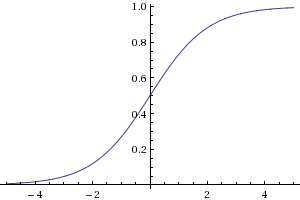
\includegraphics[width=0.6\textwidth]{logistic.png}
	\caption[Η λογιστική συνάρτηση]{Η λογιστική συνάρτηση}
\end{figure}

\paragraph{Ερμηνεία} Καθώς θέλουμε να κάνουμε μια πρόβλεψη για κάποιο άγνωστο χαρακτηριστικό με βάση κάποια άλλα χαρακτηριστικά-προβλέπτες που το αφορούν κινούμαστε στα εξής πλαίσια: αρχικά υπολογίζουμε πως επηρεάζει κάθε χαρακτηριστικό-προβλέπτης την άγνωστη ποσότητα, δηλαδή του δίνουμε κάποιο βάρος. Στη συνέχεια με βάση τα χαρακτηριστικά ενός δεδομένου παίρνουμε μία τιμή
για αυτό, την οποία θα μπορούσαμε να ερμηνεύσουμε ως το βαθμό που εμφανίζει το δεδομένο ως προς το χαρακτηριστικό που προβλέψουμε. Στη συνέχεια περνάμε αυτή τη τιμή  από ένα κατώφλι, ώστε να δούμε πού θα την κατατάξουμε. Η μαθηματική μετάφραση της παραπάνω διαδικασίας είναι η εξής:
$$s=w^T x \rightarrow h(x)=\theta(s)=\frac{e^{w^T x}}{1 + e^{w^T x} }$$
Η πραγματική πιθανότητα, που προσπαθούμε να προσεγγίσουμε  ορίζεται ως εξής:
$$P(y \mid x)=\left\{
\begin{array}{ll}
f(x)  & \mbox{if } y = +1 \\
1 - f(x)  & \mbox{if } y = -1
\end{array}
\right.$$

Αν υποθέσουμε πως η υπόθεσή μας είναι σωστή, δηλαδή $h=f$, τότε η πιθανότητα να πάρουμε έξοδο y για ένα δεδομένο με χαρακτηριστικά x είναι:
$$P(y \mid x)=\left\{
\begin{array}{ll}
h(x)  & \mbox{if } y = +1 \\
1 - h(x)  & \mbox{if } y = -1
\end{array}
\right.$$

Αν αντικαταστήσουμε με $h(x)=\theta(w^T x)$ και λαμβάνοντας υπόψιν πως $\theta(-s)= 1 - \theta(s)$, τότε η πιθανότητα  προκύπτει:
$$P(y \mid x)= \theta(y w^T x)$$
Ο παραπάνω τύπος λαμβάνει υπόψιν του μόνο ένα σημείο. Αν έχω N δεδομένα στο σετ εκπαίδευσης τότε η υπόθεσή μου γίνεται:
$$\prod_{n=1}^{N} P(y \mid x)= \prod_{n=1}^{N} \theta (y_n w^t x_n)$$
Η ερώτηση την οποία οφείλουμε να απαντήσουμε τώρα είναι : ”Δεδομένου του σετ εκπαίδευσης, ποιά είναι η πιθανότερη υπόθεση;” Η συνάρτηση, την οποία θέλουμε να ελαχιστοποιήσουμε, είναι η εξής:

$$Error(w)= \frac{1}{N} \sum_{n=1}^{N} \ln (1 + e^{- y_n w^T x_n} )$$

\paragraph{Gradient descent} Πρόκειται για έναν αλγόριθμο βελτιστοποίησης που προσπαθεί να βρει το τοπικό ελάχιστο μιας κυρτής συνάρτησης. Η διαδικασία είναι επαναληπτική και σε κάθε βήμα ο αλγόριθμος επιλέγει άπληστα να κινηθεί προς την πιο απότομη κατεύθυνση, που αντιστοιχεί στην αντίθετη κατεύθυνση της κλίσης στο συγκεκριμένο σημείο.
\begin{figure}[H]
	\centering			
%	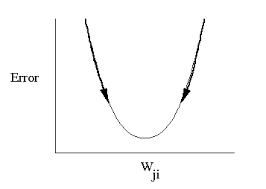
\includegraphics[width=0.6\textwidth, height=5cm]{gradient.png}
	\caption[Steepest descent]{Steepest descent}
\end{figure}
Εκτός από την κατεύθυνση προς την οποία θα κινηθεί ο αλγόριθμος πρέπει να επιλέξει και το μέγεθος του βήματος που θα εκτελέσει. Η παράμετρος αυτή επηρεάζει τόσο την ταχύτητα εκτέλεσης του αλγορίθμου, όσο και την επιτυχία του: αν τα βήματα που κάνει είναι σταθερά και μικρά, τότε θα φτάσει εγγυημένα σε κάποιο ελάχιστο, αλλά πολύ αργά, μειώνοντας την απόδοση του συστήματος. Αντιθέτως αν το βήμα είναι πολύ μεγάλο, μπορεί να υπερπηδά το ελάχιστο κάθε φορά που το πλησιάζει και ο αλγόριθμος να μην συγκλίνει ποτέ. Συνήθως υιοθετούμε μια πιο σύνθετη προσέγγιση: επιλέγουμε αρχικά μεγάλο βήμα, ώστε να πλησιάσουμε γρήγορα στη λύση και το μειώνουμε μόλις φτάσουμε κοντά.
\begin{figure}[H]
	\centering
	\begin{minipage}{.5\textwidth}
		\centering
%		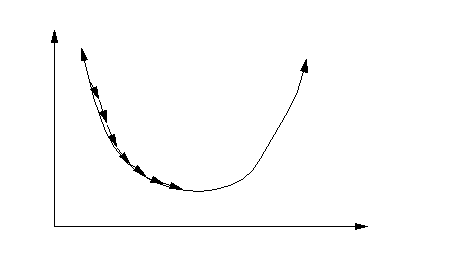
\includegraphics[width=0.8\linewidth, height=0.15\textheight]{smallstep.png}
		\caption[Gradient descent με πολύ μικρό βήμα]{Gradient descent με πολύ μικρό βήμα}
		
	\end{minipage}%
	\begin{minipage}{0.5\textwidth}
		\centering
%		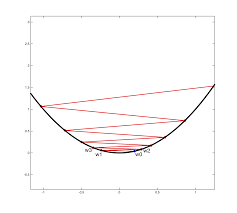
\includegraphics[width=0.8\linewidth, height=0.15\textheight]{bigstep.png}
		\caption[Gradient descent με πολύ μεγάλο βήμα]{Gradient descent με πολύ μεγάλο βήμα}
		
	\end{minipage}
\end{figure}
\chapter{Κ-κοντινότερος γείτονας}
\label{appendix:knn}
Ο αλγόριθμος αυτός ανήκει στην κατηγορία των αλγορίθμων βασισμένων σε παραδείγματα (instance-based), δηλαδή οι προβλέψεις του βασίζονται εξ ολοκλήρου στα παραδείγματα (instances) και δε λαμβάνει χώρα κάποια εκπαίδευση. Οι αλγόριθμοι αυτοί είναι πολύ χρήσιμοι σε εφαρμογές που απαιτούν online μάθηση, επειδή τα δεδομένα έρχονται σειριακά και δεν είναι διαθέσιμα σε ομάδες για εκπαίδευση, όπως σε προβλέψεις μετοχών στο χρηματιστήριο.

Η ταξινόμηση ενός σημείου με άγνωστη κλάση γίνεται ως εξής: βρίσκουμε τους k κοντινότερους γείτονές του και του αναθέτουμε την κλάση της πλειοψηφίας.

Μία σημαντική παράμετρος, που εξαρτάται από το πεδίο εφαρμογής, είναι ο τρόπος με τον οποίο υπολογίζεται η απόσταση μεταξύ των σημείων. Διάφορες επιλογές είναι:
\begin{itemize}
	\item \textit{Ευκλείδεια απόσταση.} Πρόκειται για το συνηθέστερο τρόπο υπολογισμού απόστασης και δίνεται από τον τύπο:
	\begin{equation}
	\sqrt[]{\sum_{i=1}^{Κ} (x_i - y_i )^2}
	\end{equation}
	\item \textit{Απόσταση Hamming.} Χρησιμοποιείται για κατηγορικά δεδομένα και κυρίως σε εφαρμογές επεξεργασίας κειμένου. Η απόσταση μεταξύ δύο παραδειγμάτων είναι το άθροισμα της απόστασης μεταξύ των χαρακτηριστικών τους, που ισούται με μηδέν για τα χαρακτηριστικά που συμπίπτουν και ένα για τα υπόλοιπα.
	\item \textit{Απόσταση Manhattan.} Εμπνευσμένη από την οργάνωση του Manhattan σε οικοδομικά τετράγωνα, για τον υπολογισμό της απόστασης μεταξύ δύο σημείων μπορούμε να κινηθούμε μόνο οριζοντίως ή καθέτως. Ορίζεται ως εξής:
	\begin{equation}
	\sum_{i=1}^{Ξ} \abs{x_i - y_i}
	\end{equation}
\end{itemize}

Τέλος, η επιλογή του k οφείλει να γίνει με προσοχή. Αν είναι πολύ μεγάλο υπάρχει ο κίνδυνος κατά την ταξινόμηση να λαμβάνουμε υπόψιν πολύ μακρινά παραδείγματα, ενώ αν είναι πολύ μικρό η ταξινόμηση θα επηρεάζεται εύκολα από ενδεχόμενο θόρυβο στα δεδομένα.
\paragraph{Συνάρτηση Ακτινικής βάσης }
Η συνάρτηση αυτή σχετίζεται με πολλές έννοιες της μηχανικής μάθησης. Σε αυτό το σημείο θα ορίσουμε το βασικό της μοντέλο και θα δούμε τη λειτουργία της ως τεχνική βασισμένη σε παραδείγματα. 

Η λογική του  μοντέλου αυτού είναι η εξής: η υπόθεση σε ένα σημείο επηρεάζεται από την απόστασή του από κάθε παράδειγμα του σετ εκπαίδευσης. Πιο συγκεκριμένα, η μαθηματική διατύπωση της υπόθεσης, που έχει και τη μορφή του σχήματος που ακολουθεί, είναι η εξής:
\begin{equation}
h(x)= sign( \sum_{n=1}^{N} w_n e^{-\gamma \norm{x - x_n}^2})
\end{equation}

Η επιλογή της βέλτιστης υπόθεσης έγκειται σε αυτήν που προβλέπει σωστά όλα τα παραδείγματα του σετ εκπαίδευσης. Αν και συνήθως προσπαθούμε να ελαχιστοποιήσουμε το σφάλμα, εδώ είμαστε σίγουροι πως θα καταφέρουμε να το μηδενίσουμε, καθώς το μοντέλο μας έχει στη διάθεση του πάρα πολλές παραμέτρους (όσα είναι και τα παραδείγματα). Επομένως το πρόβλημα βελτιστοποίησης ορίζεται ως:
\begin{equation}
E_{in}=0 \rightarrow  \sum_{n=1}^{N} w_n e^{-\gamma \norm{x_n - x_m}^2}= y_n  \forall n \in D_N 
\end{equation}
όπου $E_{in}$ είναι το σφάλμα στα παραδείγματα εκπαίδευσης και $D_N$ το σετ εκπαίδευσης. 

Ο παραπάνω τύπος δίνει ένα σύστημα Ν γραμμικών εξισώσεων με Ν αγνώστους που διατυπώνεται εύκολα ως εξής:
\[
\underbrace{
	\begin{bmatrix}
	e^{-\gamma \norm{x_1 - x_1}^2}  & \dots  &  e^{-\gamma \norm{x_1 - x_N}^2} \\
	e^{-\gamma \norm{x_2 - x_1}^2}  & \dots  &  e^{-\gamma \norm{x_2 - x_N}^2} \\
	\vdots  & \vdots & \vdots \\
	e^{-\gamma \norm{x_N - x_1}^2}  & \dots  &  e^{-\gamma \norm{x_N - x_N}^2} \\
	\end{bmatrix}}_{  \Phi}
\underbrace{
	\begin{bmatrix}
	w_{1}       \\
	w_{2}        \\
	\vdots        \\
	w_{N}
	\end{bmatrix}}_{W}
=
\underbrace{
	\begin{bmatrix}
	y_{1}       \\
	y_{2}        \\
	\vdots        \\
	y_{N}
	\end{bmatrix}}_{Y}
\]

Η λύση αυτού του συστήματος δίνεται από τον τύπο:
\begin{equation}
w=\inv{\Phi} y
\end{equation}

όπου ο πίνακας $\Phi$ πρέπει να είναι αντιστρέψιμος

\paragraph{Επίδραση της μεταβλητής γ} Η μεταβλητή αυτή ορίζει πόσο απλωμένη είναι η καμπάνα γύρω από κάθε σημείο του σετ εκπαίδευσης και άρα πόσο επίδραση έχει αυτό στη γειτονιά του.

\paragraph{H συνάρτηση RBF ως μοντέλο βασισμένο σε παραδείγματα.} Όπως είδαμε η ταξινόμηση ενός σημείου εξαρτάται από την απόστασή του από τα υπόλοιπα του σετ εκπαίδευσης, τεχνική που παραπέμπει άμεσα στη λογική της κατηγοριοποίησης με βάση τα παραδείγματα. Μέχρι τώρα έχουμε θεωρήσει ως συνάρτηση βάσης την γκαουσιανή, αν όμως τοποθετήσουμε έναν απλό κύλινδρο γύρω από κάθε σημείο, η τεχνική αυτή ταυτίζεται με το μοντέλο k-NN.
\paragraph{Επιλογή Κ κέντρων.} Η χρήση τόσων παραμέτρων όσων είναι και τα στοιχεία του σετ εκπαίδευσης κάνει τη διαδικασία της εκπαίδευσης χρονοβόρα και ενέχει κινδύνους υπερπροσαρμογής. Συνήθως λοιπόν χρησιμοποιούμε μια τροποποίηση της τεχνικής που έχουμε περιγράψει, όπου αντί να υπολογίζουμε την απόσταση από όλα τα σημεία, επιλέγουμε Κ αντιπροσωπευτικά σημεία του χώρου και τους αναθέτουμε κάποια από τα σημεία του σετ εκπαίδευσης. Έτσι, σχηματίζονται ομάδες σημείων που αντιπροσωπεύονται από το κέντρο τους και απαιτείται πλέον ο καθορισμός Κ και όχι Ν παραμέτρων.

Πλέον η υπόθεση δίνεται από τον τύπο:
\begin{equation}
h(x)= sign( \sum_{k=1}^{K} w_n e^{-\gamma \norm{x - \mu_k}^2})
\end{equation}

όπου $\mu_k$ είναι το κέντρο μιας ομάδας. Η επιλογή των βαρών $w_n$ είναι παρόμοια: έχω Ν εξισώσεις και Κ παραμέτρους, οπότε το σύστημα λύνεται με τη χρήση του ψευδοαντίστροφου πίνακα:
\begin{equation}
w= \inv{\Phi^T \Phi} \Phi^T y
\end{equation}
\fbox{\begin{minipage}{\textwidth}
		\begin{center}
			Επίλυση υπερ-ορισμένων συστημάτων με χρήση ψευδοαντίστροφου
		\end{center} 
		Ένα γραμμικό σύστημα $y=A x$ χαρακτηρίζεται ως υπερ-ορισμένο όταν έχει περισσότερες εξισώσεις από αγνώστους. Σε αυτή τη περίπτωση ο πίνακας Α είναι μη τετραγωνικός και επομένως μη αντιστρέψιμος, οπότε η λύση δεν μπορεί να δοθεί ως συνήθως από $x=\inv{A} y$. Μία συνήθης λύση είναι η χρήση του ψευδοαντίστροφου Moore-Penrose~\footnote{https://en.wikipedia.org/wiki/Moore\%E2\%80\%93Penrose\_pseudoinverse}, που ορίζεται ως $ A\ssymbol{2}\ = \inv{(A^T A)} A^T$, ώστε να ισχύει $A\ssymbol{2}\ Α = I $, αλλά όχι $Α A\ssymbol{2} \= I$. Τότε, ο πολλαπλασιασμός και των δύο μερών της εξίσωσης με $ A\ssymbol{2}\ $ δεν εγγυάται ισότητα, αλλά προσέγγιση ελαχίστων τετραγώνων και η λύση είναι $x \approx A\ssymbol{2}\ y $
	\end{minipage}}
	
	Το νέο πρόβλημα που αναδύεται είναι αυτό της επιλογής των βέλτιστων $\mu_k$. Το πρόβλημα αυτό επιλύεται με την τεχνική της k-means ομαδοποίησης και διατυπώνεται ως εξής: Πρέπει να διαχωρίσουμε τα σημεία $x_1,..., x_n$ σε k ομάδες $S_1,...,S_k$, ώστε να ελαχιστοποιήσουμε το μέγεθος:
	\begin{equation}
\sum_{k=1}^{K} \sum_{x_n \in S_k} \norm{x_n - \mu_k}^2
\end{equation}
	που δίνει το άθροισμα των αποστάσεων κάθε σημείου από το κέντρο της ομάδας στην οποία ανήκει.
	
	Η συνηθέστερη λύση του δίνεται από τον αλγόριθμο του Lloyd \citep{Lloyd:2006:LSQ:2263356.2269955}, που εντοπίζει ένα τοπικό ελάχιστο επαναληπτικά σπάζοντας τη διαδικασία σε δύο ανεξάρτητα στάδια:
	\begin{itemize}
		\item \textit{υπολογισμός κέντρων.} Δεδομένων των ομάδων, το κέντρο κάθε ομάδας παίρνει την μέση τιμή των σημείων που της ανήκουν.
		\item \textit{υπολογισμός ομάδων.} Για κάθε σημείο του σετ εκπαίδευσης υπολογίζουμε την απόστασή του από το κέντρο κάθε ομάδας και το αναθέτουμε στην κοντινότερη ομάδα.
	\end{itemize}
	
	Η διαδικασία επαναλαμβάνεται μέχρι να συγκλίνουμε σε μια ομαδοποίηση των σημείων, δηλαδή οι ομάδες να μη μεταβάλλονται σε μια επανάληψη του αλγορίθμου.
\chapter{Κανονικοποίηση}
\label{appendix:Reg}
\paragraph{Διακύμανση - Πόλωση Μοντέλου}
Κατά την επιλογή του μοντέλου που θα χρησιμοποιήσουμε για μια εφαρμογή μηχανικής μάθησης, το βασικό δίλημμα μπροστά στο οποίο βρισκόμαστε είναι αυτό της πολυπλοκότητας της υπόθεσης. Το γεγονός πως προσπαθούμε να προσεγγίσουμε μία άγνωστη συνάρτηση και η αμφιβολία που νιώθουμε για την αξιοπιστία των δεδομένων μας καθιστούν τη λήψη της απόφασης ενστικτώδη και ριψοκίνδυνη. Στο παρακάτω παράδειγμα, έχουμε κάποια δισδιάστατα δεδομένα για ένα πρόβλημα παλινδρόμησης και θέλουμε να επιλέξουμε μεταξύ δύο μοντέλων:

\begin{figure}[!htb]
	\centering			
	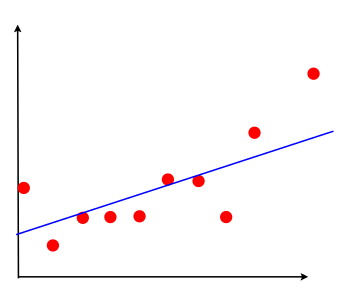
\includegraphics[scale=0.5]{bias}
	\caption[Μοντέλο υψηλής πόλωσης]{Μοντέλο υψηλής πόλωσης}
\end{figure}

Η πρώτη επιλογή μας συνιστά μία ευθεία, δηλαδή ένα πολυώνυμο πρώτης τάξης, το οποίο καθορίζεται από δύο παραμέτρους. Παρατηρούμε πως το μοντέλο αυτό είναι τόσο απλό, που όσο και να προσπαθήσουμε δε θα καταφέρει να προβλέψει καλά τα δεδομένα μας. Θα ήταν ουτοπικό να χαρακτηρίζεται κάποιο πραγματικό φαινόμενο από μια τόσο απλή συνάρτηση, οπότε θα απορρίπταμε αυτό το μοντέλο ως υψηλά πολωμένο, καθώς κάνει μια σημαντική υπόθεση απλότητας.

\begin{figure}[!htb]
	\centering			
	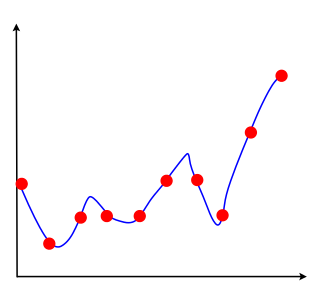
\includegraphics[scale = 0.5]{variance}
	\caption[Μοντέλο υψηλής διακύμανσης]{Μοντέλο υψηλής διακύμανσης}
\end{figure}

Η δεύτερη επιλογή μας είναι ένα πολυώνυμο υψηλής τάξης, το οποίο μπορεί εύκολα να επιδείξει μηδενικό σφάλμα στα δεδομένα εκπαίδευσης που διαθέτουμε. Το μοντέλο αυτό είναι φαινομενικά τέλειο και αναπόφευκτα προκαλεί αμφιβολίες: είναι όλα τα δεδομένα μας τόσο αξιόπιστα και χαρακτηριστικά για το φαινόμενο που προβλέπουμε, ώστε να αξίζει να τα προσεγγίσουμε τέλεια; Γενικά, δεδομένα πολύ υψηλής διακύμανσης είναι ύποπτα για θόρυβο, ο οποίος ως τυχαίος είναι συχνά υψίσυχνος, σε αντίθεση με φυσικά δεδομένα που υπακούν σε κάποιες συνθήκες ομαλότητας. Μήπως λοιπόν στην προσπάθειά μας να προβλέψουμε καλά την άγνωστη συνάρτηση παρασυρθήκαμε και μοντελοποιήσαμε το θόρυβο; Ένα τέτοιο μοντέλο είναι καταδικασμένο να αποτύχει σε καινούρια δεδομένα και χαρακτηρίζεται ως μοντέλο υψηλής διακύμανσης. Το παραπάνω πρόβλημα είναι αυτό που έχουμε αποκαλέσει υπερ-προσαρμογή.

Ο θόρυβος, που μας παρασύρει σε υπερ-προσαρμογή, αποτελείται από δύο συνιστώσες: το στοχαστικό θόρυβο, ο οποίος εμφανίζεται τυχαία στα δεδομένα μας και χαρακτηρίζεται από μία κατανομή $\epsilon(x)$ και τον ντετερμινιστικό. Ο τελευταίος οφείλεται στην πολυπλοκότητα της συνάρτηση-στόχου: το μοντέλο ερμηνεύει ως θόρυβο οποιαδήποτε διακύμανση δεν μπορεί να μοντελοποιήσει, καθώς είναι πολύ πολύπλοκη για αυτό, είτε αυτή γεννήθηκε τυχαία είτε προήλθε από τη συνάρτηση-στόχο.

Η μαθηματική αποτύπωση του παραπάνω προβλήματος έχει ως εξής: αν επιλέξουμε ένα μοντέλο $g(x)$ για να προβλέψουμε μια συνάρτηση $f(x)$ και ορίσουμε ως $\bar{g}(x)$ την καλύτερη δυνατή πρόβλεψη που μπορεί να κάνει το μοντέλο δεδομένων των παραμέτρων που περιέχει και της πολυπλοκότητας της $f(x)$ και $g_D(x)$ όλες τις πιθανές υποθέσεις που είναι σε θέση να κάνει το μοντέλο, ρυθμίζοντας τις παραμέτρους του, τότε το σφάλμα στο σετ εκπαίδευσης μπορεί να χαρακτηρισθεί ως εξής:
	\begin{equation}
	E_{error}=\underbrace{E_x(g_D(x) - g(x))^2}_{\text{σφάλμα λόγω  διακύμανσης}} + \underbrace{E_x(\bar{g}(x)- f(x))^2}_{\text{σφάλμα λόγω πόλωσης}} + E_{\epsilon,x}(\epsilon(x^2))
	\end{equation}
\paragraph{Η ιδέα της κανονικοποίησης} Η τεχνική της κανονικοποίησης στοχεύει στη μείωση της διακύμανσης με ταυτόχρονη διατήρηση χαμηλής πόλωσης. Ουσιαστικά προσπαθεί να διατηρήσει την πολυπλοκότητα της υπόθεσης, διατηρώντας το
ίδιο πλήθος παραμέτρων, ώστε να έχει τη δυνατότητα να προβλέψει μια πολύπλοκη συνάρτηση-στόχο, περιορίζοντας ωστόσο την επιλογή των τιμών των παραμέτρων, ώστε να δυσκολεύεται να προβλέψει το θόρυβο.



\chapter{Στατιστικά τεστ Υπόθεσης}
\label{appendix:Tests}
Γενικά χαρακτηριστικά των στατιστικών τεστ υπόθεσης έχουν περιγραφεί στην Ενότητα \ref{section:tests}. Σε αυτό το σημείο θα αναφέρουμε περιληπτικά μερικά είδη τέτοιων τεστ, τα οποία διαφοροποιούνται κυρίως ως προς:
\begin{itemize}
	\item τις υποθέσεις που κάνουν για τους πληθυσμούς.
	\item τη στατιστική που χρησιμοποιούν για να περιγράψουν το δείγμα.
\end{itemize}
\paragraph{Pearson's Chi-squared τεστ}
Πρόκειται για ένα στατιστικό τεστ μεταξύ δύο συνόλων κατηγορικών δεδομένων που εξετάζει αν οι διαφορές τους προκλήθηκαν τυχαία. Είναι κατάλληλο για μη-ζευγαρωμένα (unpaired) δεδομένα από μεγάλα δείγματα. Προέρχεται από την ευρύτερη οικογένεια των τεστ που αξιολογούνται με αναφορά στην κατανομή chi-squared, για την οποία όταν η μηδενική υπόθεση είναι αληθής η κατανομή του test statistic είναι chi-squared~\footnote{https://en.wikipedia.org/wiki/Chi-squared\_test}. 
\paragraph{Yate's correction for continuity}
Η τεχνική αυτή χρησιμοποιείται για διόρθωση του εξής προβλήματος: κατά την εφαρμογή του Pearson's chi-squared τεστ γίνεται η υπόθεση πως η διακριτή πιθανότητα των παρατηρούμενων συχνοτήτων στον πίνακα ενδεχομένων μπορεί να προσεγγιστεί από μία συνεχή chi-squared κατανομή.
\paragraph{ANOVA τεστ} Εισήχθη στο \citet{QJ:QJ49708235130} ως μία τεχνική ανάλυσης των διαφορών που παρουσιάζονται στις μέσες τιμές διαφορετικών ομάδων. Στην περίπτωση που οι ομάδες είναι ανεξάρτητες χρησιμοποιείται η one-way εκδοχή, ενώ όταν υπάρχει κάποια συσχέτιση μεταξύ τους η repeated-measures. Το τεστ αυτό χρησιμοποιείται για την περίπτωση σύγκρισης περισσότερων των τριών πληθυσμών, καθώς πολλαπλά t-tests θα οδηγούσαν σε μη αποδεκτό σφάλμα τύπου Ι. 

Προκειμένου να ορίσει το F-statistic η τεχνική αυτή αναλύει τη διακύμανση που εμφανίζεται στο πληθυσμό σε αυτή που οφείλεται σε διαφορές μεταξύ των διαφορετικών ομάδων και διαφορές εντός των ομάδων, δηλαδή διαχωρίζει τις πηγές διακύμανσης. Οι υποθέσεις που κάνει αυτό το τεστ είναι:
\begin{itemize}
	\item Κανονική κατανομή της εξαρτημένης μεταβλητής για κάθε ομάδα.
	\item Υπάρχει ομοιογένεια στις διακυμάνσεις, δηλαδή είναι ίσες για κάθε ομάδα.
	\item Οι παρατηρήσεις είναι ανεξάρτητες, γεγονός που καθορίζεται κατά τη συλλογή των δεδομένων.
\end{itemize}

\paragraph{Friedman τεστ}
Πρόκειται για ένα μη-παραμετρικό τεστ για την ανίχνευση διαφορών μεταξύ πολλών αλγορίθμων σε πολλά σετ δεδομένων. Θεωρείται μια μη-παραμετρική εκδοχή της ANOVA, με απόρροια την απεμπλοκή από τις υποθέσεις της κανονικής κατανομής, των ίσων διακυμάνσεων των residuals και την απώλεια ισχύος.  

Σημαντική προσθήκη αποτελεί η εναλλακτική test statistic που εισήγαγαν οι \citet{doi:10.1080/03610928008827904}, καθώς διαπίστωσαν ότι η βασική ήταν ανεπιθύμητα συντηρητική. 

Σε περίπτωση διαπίστωσης σημαντικής στατιστικής διαφοράς στην απόδοση πολλών αλγορίθμων προκύπτει η ανάγκη εξακρίβωσης των ζευγαριών που οδήγησαν σε αυτό το αποτέλεσμα. Προς αυτό το σκοπό μπορούν να χρησιμοποιηθούν τα εξής post-hoc τεστ: η διαδικασία Tukey, το Dunnett τεστ, η διόρθωση Bonferroni, το τεστ Nemenyi, η προς-τα-κάτω διαδικασία του Holm, η διαδικασία του Hommel \citep{CIS-57999, citeulike:4294367, doi:10.1093/biomet/75.2.383}.
\paragraph{Fisher's exact τεστ}
 Εισήχθη από τον Fisher μέσω του παραδείγματος της Κυρίας που δοκιμάζει Τσάι~\footnote{https://en.wikipedia.org/wiki/Lady\_tasting\_tea} ως ένα τεστ για κατηγορικά δεδομένα, τα οποία κατατάσσονται μεταξύ δύο κατηγοριών. Σύμφωνα με την ανάλυση η μηδενική υπόθεση αντιστοιχεί σε υπερ-γεωμετρική κατανομή των δεδομένων.
  
 Χρησιμοποιείται κυρίως στην περίπτωση μικρών δειγμάτων. Λέγεται ακριβές επειδή για μικρά δείγματα η σημασία της διακύμανσης από τη μηδενική υπόθεση (p-value) μπορεί να υπολογιστεί ακριβώς αντί να βασίζεται σε μια προσέγγιση που γίνεται ακριβής καθώς το μέγεθος του δείγματος πλησιάζει το άπειρο.
\paragraph{Mann–Whitney U τεστ (Wilcoxon rank-sum)} Εισήχθη από τον \citet{Wilcoxon45} και αναλύθηκε διεξοδικά από τους \citet{mann1947}. Πρόκειται για ένα μη-παραμετρικό τεστ της μηδενικής υπόθεσης ότι είναι εξίσου πιθανό μία τυχαία επιλεγμένη τιμή από ένα δείγμα να είναι μικρότερη ή μεγαλύτερη από μία επιλεγμένη τιμή από ένα άλλο δείγμα. Σε αντίθεση με το t-test δεν απαιτεί κανονικότητα των πληθυσμών.
 
\paragraph{McNemar}
Εισήχθη από τον \citet{McNemar1947} ως ένα τεστ για ζευγαρωμένα ονομαστικά δεδομένα, δηλαδή δεδομένα που διαφοροποιούνται μόνο από το όνομά τους και υπάρχει ένα-προς-ένα συσχέτιση μεταξύ τους.

\paragraph{Cochran-Mantel-Haenszel} Συνδιαμορφώθηκε από τους \citet{10.2307/3001616, doi:10.1093/jnci/22.4.719} και αποτελεί γενίκευση του McNemar, καθώς υποστηρίζει διαστρωμάτωση των δεδομένων σε αυθαίρετο πλήθος ομάδων.
\chapter{Αλγόριθμοι }
\label{appendix:Alg}

\begin{myalgorithm}[H]
	\For{n=1 μέχρι N }{
		βρες το $x_{n+1}$ ως το σημείο που μεγιστοποιεί τη συνάρτηση απόκτησης \;
		υπολόγισε το αντίστοιχο $y_{n+1}$ από τη συνάρτηση κόστους\;
		ανανέωσε το στατιστικό μοντέλο με το νέο σημείο $(x_{n+1}, y_{n+1})$\;
	}
	\caption{Ψευδοκώδικας Bayesian Βελτιστοποίησης}
\end{myalgorithm}

\begin{myalgorithm}[H]
	H=0\;
	\For{t=1 μέχρι Τ }{
		βρες τo $\theta^*=argmin S(\theta, M_{t-1})$ \;
		υπολόγισε το $f(\theta^*)$\;
		Ανανέωσε το σετ εκπαίδευσης $H=H \cup (\theta^*, f(\theta^*)) $\;
		Εκπαίδευσε ένα νέο μοντέλο $M_t$ στο Η \;
	}
	\caption{Ψευδοκώδικας SΜΒΟ}
\end{myalgorithm}
\chapter{Εξαγωγή διαστημάτων πρόβλεψης από μοντέλα παλινδρόμησης}
\label{appendix:Intervals}

Το διάστημα πρόβλεψης αποτελεί μια εκτίμηση για το διάστημα στο οποίο θα βρεθούν μελλοντικές παρατηρήσεις ενός πληθυσμού με μία συγκεκριμένη πιθανότητα.

Αν θεωρήσουμε μία κανονική κατανομή  $\mathcal{N} (\mu, \sigma)$, τότε το διάστημα πρόβλεψης για πιθανότητα $\gamma$ προκύπτει με τη βοήθεια της τυπικής κανονικής κατανομής Z, για την οποία τα τεταρτημόρια είναι προ-υπολογισμένα.
\begin{equation}
\gamma = P\big(l < X < u\big) = P\Bigg(\frac{l-\mu}{\sigma} < \frac{X-\mu}{\sigma} < \frac{u-\mu}{\sigma}\Bigg)= P\Bigg(\frac{l-\mu}{\sigma} < Z < \frac{u-\mu}{\sigma}\Bigg)
\end{equation}

Επομένως
\begin{equation}
\frac{l-\mu}{\sigma} = -z \qquad\text{και}\qquad \frac{u-\mu}{\sigma} = -z
\end{equation}

και το διάστημα πρόβλεψης ορίζεται ως:
\begin{equation}
	[\mu - z \sigma, \mu + z \sigma ]
\end{equation}

\paragraph{Από γραμμικό μοντέλο}
Κατά την εκπαίδευση ενός γραμμικού μοντέλου συνίσταται η επίδειξη κανονικότητας των residuals του μοντέλου, προκειμένου να είναι δυνατός ο υπολογισμός των διαστημάτων πρόβλεψης μέσω της κανονικής κατανομής.

Αν θεωρήσουμε ότι έχουμε $n$ παραδείγματα και $s_y$ είναι η τυπική απόκλιση των residuals του μοντέλου, η οποία ορίζεται ως:
\begin{equation}
\sqrt{\frac{\sum(y_i - \hat{y_i})^2}{n-2}}
\end{equation}
τότε το διάστημα πρόβλεψης δίνεται από τον τύπο:
\begin{equation}
\hat{y}\pm t^*_{n-2} s_y \sqrt{1 + \frac{1}{n} + \frac{(x^* - \bar{x})^2}{(n-1) s_x^2}}
\end{equation}
όπου ο όρος $t$ αντιστοιχεί στο δείκτη t value, το t-statistic της μηδενικής υπόθεσης ο συντελεστής του μοντέλου παλινδρόμησης να είναι μηδενικός.   

[ΒΑΛΕ ΚΑΙ ΑΛΛΑ ΣΤΑΤΙΣΤΙΚΣ ΚΑΙ ΟΝΟΜΑΣΕ ΑΥΤΟ ΠΟΥ ΧΡΗΣΙΜΟΠΟΙΗΣΕΣ]

\paragraph{Από SVM} Ένα μοντέλο παλινδρόμησης παραγόμενο με SVM διαφέρει από ένα συμβατικό γραμμικό μοντέλο ως προς τον τρόπο διαχείρισης των δεδομένων, τα οποία μετασχηματίζει σε ένα νέο χώρο σύμφωνα με τη συνάρτηση πυρήνα. Ως αποτέλεσμα οι τεχνικές εξαγωγής διαστημάτων πρόβλεψης που περιγράψαμε δεν είναι εφαρμόσιμες.

Η βιβλιογραφία περιέχει διάφορες προσπάθειες απόδοσης πιθανοτικής εξόδου στον αλγόριθμο SVM, όπως ο αλγόριθμος του \citet{Platt99probabilisticoutputs} για μοντέλα ταξινόμησης και η μέθοδος των \citet{Jiang:2008:ECI:1390681.1390698} και \citet{Lin04simpleprobabilistic} για παλινδρόμησης. Εμείς βασίσαμε τα πειράματά μας στη δεύτερη μέθοδο, καθώς εφαρμόζεται από την επικρατέστερη βιβλιοθήκη εκπαίδευσης SVM μοντέλων, τη LIBSVM~\footnote{https://www.csie.ntu.edu.tw/~cjlin/libsvm/}, η οποία επίσης αποτελεί τη βάση της βιβλιοθήκης kernlab που χρησιμοποιήσαμε.

Η μέθοδος αυτή μοντελοποιεί τα σφάλματα των προβλέψεων (residuals) ως
\begin{equation}
\zeta = y - \hat{f(x)}
\end{equation}

όπου y η κλάση μίας παρατήρησης και $\hat{f}(x)$ η πρόβλεψη για αυτήν. Στόχος της ανάλυσης είναι η εύρεση της κατανομής της τυχαίας μεταβλητής $\zeta$, ώστε η κατανομή του $y$ να προκύψει από τη συνέλιξη των επιμέρους κατανομών. 

Όπως περιγράφουν οι \citet{Chang:2011:LLS:1961189.1961199} ,ο υπολογισμός της κατανομής γίνεται παράγοντας τα σφάλματα εκτός δείγματος (out-of-sample residuals) με τη χρήση cross-validation και αναγνωρίζοντας την κατανομή που τα περιγράφει. Σύμφωνα με τα πειράματα των \citet{Lin04simpleprobabilistic} καταλληλότερη κατανομή είναι η λαπλασιανή, η οποία για τυχαία μεταβλητή $z$ περιγράφεται από τον τύπο
\begin{equation}
	p(z) = \frac{1}{2\sigma} e^{-\frac{\abs{z}}{\sigma}}
	\label{eq:laplace}
\end{equation} 
όπου $\sigma$ η παράμετρος κλιμάκωσης (scale parameter), η τιμή της οποία δίνεται από τη τεχνική της μέγιστης πιθανοφάνειας ως:
\begin{equation}
\sigma = \frac{\sum_{i=1}^{l} \abs{\zeta_{i}}}{l}
\end{equation}
όπου $l$ το πλήθος των residuals.

Για να υπολογίσουμε το διάστημα πρόβλεψης με βεβαιότητα $1-2\sigma$ θα χρειαστεί να προσδιορίσουμε το $\sigma$-μόριο της κατανομής, $p_s$, το οποίο στη γενική περίπτωση μιας συμμετρικής μεταβλητής Z δίνεται από τον τύπο
\begin{equation}
\int_{-\infty}^{p_z}p(z)dz = 1-s
\end{equation}
που με χρήση της σχέσης \ref{eq:laplace} δίνει το διάστημα
\begin{equation}
	(\sigma \ln{2 s}, -\sigma \ln{2 s})
\end{equation}


	\chapter{Σετ δεδομένων }
\label{appendix:Datasets}
{ \footnotesize
	 	\begin{longtable}{|l| l| l | l | l | l |l | l | l | } 
 			\hline
 			 & Όνομα & Πηγή & Πεδίο & Τύπος & { Π.Π} & {Π.Χ} & Κλάση & NAs \\
 			\hline
 							\rownumber  & accident \citep{accident} & kaggle & N/A  & csv & 2001  & 51 &  continuous & Ναι \\
 							\rownumber & ad \citep{ad} & UCI & Computer  & data & 3279 &  1558 & binary & Ναι\\
 							\rownumber & adni\_demographic & kaggle & N/A & csv & 3013 &5 &multiclass &Όχι\\
 							\rownumber &  adult  \citep{census}  & UCI & social & data  & 48842 & 14 & binary & Ναι\\
 							\rownumber &  adult-stretch  \citep{balloons} & UCI & social & data & 16 & 4 & binary & Όχι\\
 							\rownumber &  adult+stretch  \citep{balloons} & UCI & social & data & 16 & 4 & binary & Όχι\\
 							\rownumber &  AP\_Endometrium\_Breast \citep{breast} & openml & N/A & arff & 405 & 10937 & binary & Όχι\\
 							\rownumber & AP\_Endometrium\_Lung \citep{lung} & openml & N/A & arff  & 195 & 10937 & binary  & Όχι\\
 							\rownumber &  AP\_Endometrium\_Omentum \citep{omentum} & openml & N/A & arff & 138 & 10937 & binary & Όχι \\
 							\rownumber & arsenic-male-bladder \citep{bladder} & openml & N/A & arff & 559 & 5 & binary & Όχι\\
 							\rownumber & Attribute\_DataSet & UCI & Computer & xlsx & 501 & 13 & binary  & Ναι \\
 							\rownumber & australian \citep{australian} & UCI  & Financial & 690 & 14 &  dat & binary & Ναι \\
 							\rownumber & baboon\_mating \citep{baboon} & kaggle & N/A & csv & 12141& 20& binary & Όχι\\
 							\rownumber &  bands \citep{bands} & UCI & Physical & data & 512 & 39& multiclass & Όχι\\
 							\rownumber & bank-additional & UCI & csv & business & 2002 & 20 & binary & Ναι \\
 							\rownumber &  bank-additional-full & UCI & csv& business & 45211& 20& binary& Ναι \\
 							\rownumber &  biodeg \citep{biodeg} & UCI & N/A& csv &1055 & 41  & binary & Όχι \\
 							\rownumber & block\_1 & & & & & & & \\
 							\rownumber & block\_2 & & & & & & & \\
 							\rownumber & block\_3 & & & & & & & \\
 							\rownumber & block\_4 & & & & & & & \\
 							\rownumber & block\_5 & & & & & & & \\
 							\rownumber & block\_6 & & & & & & & \\
 							\rownumber & block\_7 & & & & & & & \\
 							\rownumber & block\_8 & & & & & & & \\
 							\rownumber & block\_10 & & & & & & & \\
 							\rownumber & car \citep{car} & UCI & N/A & data & 1728 & 6  & binary & Όχι\\
 							\rownumber & chess & rel. & Sport & mysql  & 296 & 19 & binary & Όχι \\
 							\rownumber & chscase\_health \citep{health} & openml & N/A & arff & 50&5 & binary & Όχι \\
 							\rownumber & cities\_r2 \citep{indian} & kaggle & N/A & csv & 494 & 21 & continuous & Όχι \\
 							\rownumber & confidence \citep{confidence}  & openml & N/A & arff & 72 & 4 &2 & Όχι \\
 							\rownumber & creditcard \citep{creditcard} & kaggle & N/A & csv & 284808 & 30 & binary & Όχι \\
 							\rownumber & crx \citep{credit}  & UCI & N/A & data & 125 & 15 & binary & Ναι \\
 							\rownumber & data\_banknote\_authentication\citep{banknote} & UCI & computer  &txt &1372 &5 & binary  & Όχι  \\
 							\rownumber & datatest & UCI & Computer & txt & 20560 & 7 & binary & Όχι \\
 							\rownumber & datatest2 & UCI & Computer & txt & 20560 & 7 & binary & Όχι \\
 							\rownumber & datatraining & UCI & Computer & txt & 20560 & 7 & binary & Όχι \\
 							\rownumber & dbworld\_bodies & UCI & Computer & arff & 64 & 4702 & binary & Όχι \\
 							\rownumber & dbworld\_bodies\_stemmed & UCI & Computer & arff & 64 & 4702 & binary & Όχι \\
 							\rownumber & dbworld\_subjects & UCI & Computer & arff & 64 & 4702 & binary & Όχι \\
 							\rownumber & dbworld\_subjects\_stemmed & UCI & Computer & arff & 64 & 4702 & binary & Όχι \\
 							\rownumber & dcg \citep{dcg} & rel. & Synthetic & mysql & 7129 & 3 & & \\
 							\rownumber & default\_of\_credit\_card\_clients \citep{default} & UCI & Business & xls & 30000 & 24 & binary & Όχι \\
 							\rownumber & dermatology \citep{dermatology} & UCI & Life & data & 366 & 33 & multi & Ναι \\
 							\rownumber & diagnosis\citep{Czerniak2003} & UCI & Life &data & 120 &10 & binary & Όχι \\
 							\rownumber & fertility\_Diagnosis & UCI & Life & txt & 100 & 10 & binary & Όχι \\
 							\rownumber & ftp \citep{ftp} & rel. & Synthetic & mysql & 29555  & 2 & binary  & Ναι  \\
 							\rownumber & gym \citep{gym} & kaggle & N/A & csv & 26067 & 6 & continuous & Όχι \\
 							\rownumber & haberman \citep{haberman} & UCI & Life & data &  306 & 3 & binary & Όχι \\
 							\rownumber & heart\citep{heart} & UCI & Life &dat & 270&13 &binary & Όχι \\
 							\rownumber & hepatitis \citep{hepatitis} & UCI & Life & data & 155 & 19 & binary & Ναι \\
 							\rownumber & Hill\_Valley\_with\_noise\_Training & UCI & N/A & data & 606 & 101 & binary & Όχι \\
 							\rownumber & Hill\_Valley\_without\_noise\_Training & UCI & N/A & data & 606 & 101 & binary & Όχι \\
 							\rownumber & house-votes-84 & UCI & Social & data & 435 & 16  & binary & Ναι  \\
 							\rownumber & HR\_comma\_sep \citep{hr} & kaggle & N/A & csv & 15000 & 9 & multi & Όχι \\
 							\rownumber & imdb \citep{imdb} & rel. & Real & mysql & 986583 & 5 & continuous & Όχι \\
 							\rownumber & indian\_ilpd & UCI & Life & csv & 583 & 10 & binary & Όχι \\
 							\rownumber & ionosphere \citep{ionoshpere} & UCI & Physical & data  & 351 & 34  &  binary & Όχι \\
 							\rownumber & kohkiloyeh & UCI & computer& xlsx& 100 & 6 & binary & Όχι \\
 							\rownumber & krk \citep{krk} & rel. & Synthetic & mysql & 1000  & 6 & binary & Όχι \\
 							\rownumber & lupus \citep{lupus} & openml & N/A & arff & 87 & 4 & binary & Όχι \\
 							\rownumber & lymphoma\_2classes & openml & N/A & arff & 45 &4027 & binary& Nαι\\
 			\rownumber & magic04 & UCI & Physical & data & 19020 & 11 & binary & Όχι \\
 			\rownumber & mammographic\_masses & UCI & Life & data & 961 & 6 & binary & Ναι \\
 			\rownumber & messidor\_features\citep{messidor} & UCI & Life & arff &1151 &20 &binary &Όχι \\
 			\rownumber & monks-1.train \citep{monks} & UCI & N/A & txt & 432 & 7 & binary & Όχι \\
 			\rownumber & monks-2.train \citep{monks} & UCI & N/A & txt & 432 & 7 & binary & Όχι \\
 			\rownumber & monks-3.train \citep{monks}& UCI & N/A & txt & 432 & 7 & binary & Όχι \\
 			\rownumber & mushrooms \citep{mushroom} & kaggle & N/A & csv & 8125 & 22 & binary & Ναι \\
 			\rownumber & musk \citep{musk} & rel. & Real & mysql & 6599
 			  & 6598 & binary & Όχι \\
 			\rownumber & mutagenesis \citep{Mutagenesis} & rel. & Real & mysql & 5244 & 16 & binary & Όχι \\
 			\rownumber & numeric sequence \citep{sequence} & kaggle & N/A & csv & 2401 & 28 & binary & Όχι \\
 			\rownumber & nursery \citep{nursery} & UCI & social & data & 12960 & 8 & multi & Όχι \\
 			\rownumber & parkinsons \citep{parkinsons} & UCI & Life & data & 197 & 23 & binary & Όχι \\
 			\rownumber & php3BOEY5 \citep{pie} & openml & N/A & arff & 745  & 37  &  binary& Όχι \\
 			\rownumber & php4ylQmK \citep{thyroid} & UCI & Life & csv & 195 & 23 & binary & Όχι \\
 			\rownumber & php7E9bQN & openml & N/A & arff & & & & \\
 			\rownumber & php9xWOpn & openml & N/A & arff & & & & \\
 			\rownumber & phphHV8xl & openml & N/A & arff & & & & \\
 			\rownumber & phpjG28NS & openml & N/A & arff & & & & \\
 			\rownumber & phpLalDwz & openml & N/A & arff & & & & \\
 			\rownumber & phplN67dW & openml & N/A & arff & & & & \\
 			\rownumber & phpqZOQcc & openml & N/A & arff & & & & \\
 			\rownumber & phps53v4E & openml & N/A & arff & & & & \\
 			\rownumber & phpSRnbqC \citep{planning} & openml & N/A & arff & 182 & 12 & binary & Όχι \\
 			\rownumber & phpZeLjnh & openml & N/A & arff & & & & \\
 			\rownumber & phpjG28NS & openml & N/A & arff & & & & \\
 			\rownumber & phpR4hXE4 & openml & N/A & arff & 3772 & 29 & binary & Όχι \\
 			\rownumber & pima-indians-diabetes \citep{pima} & UCI & Life & data & 768 & 8 & binary & Ναι \\
 			\rownumber & Pokemon & data.world& N/A& csv & 800 & 13 & binary& Ναι\\
 			\rownumber & Political-media-DFE & data.world & N/A & csv & 5000 & 22  & binary& Όχι \\
 			\rownumber & prostate\_TumorVSNormal & openml & N/A & arff & 136 & 12601  & binary & Όχι \\
 			\rownumber & ptc \citep{Helma2001} & rel.& Real  & mysql & 18313 & 6 & binary & Όχι \\
 			\rownumber & Qualitative\_Bankruptcy \citep{bankruptcy} & UCI & Computer & arff & 250 & 7 & binary & Όχι \\
 			\rownumber & rabe\_97 \citep{rabe} & openml & N/A & arff & 46 & 5 & binary & Όχι \\
 			\rownumber & reviews & kaggle & N/A & csv & 9188&8 & multiclass & Ναι \\
 			\rownumber & SalesKaggle3 \citep{sales} & kaggle & N/A & csv & 198918 & 14 & continuous & Όχι \\
 			\rownumber & seismic-bumps \citep{seismic} & UCI & N/A & arff & 2584 & 19& binary & Όχι \\
 			\rownumber & shuttle-landing-control \citep{shuttle} & UCI & Physical & data & 15  & 6 & binary &  Όχι \\
 				\rownumber & sonar & UCI & Physical & data & 208 & 60 & binary  & Όχι \\
 				\rownumber & spambase \citep{spam} & UCI & Computer & data & 4601 & 57 & binary & Ναι  \\
 				\rownumber & SPECTF \citep{spectf} & UCI & Life & data & 267 & 44 & binary & Όχι \\
 				\rownumber & student-mat \citep{alcohol} & kaggle & N/A & csv & 396 & 32 & multi & Όχι \\
 				\rownumber & testing \citep{wilt} & UCI & Life & csv & 500 & 5 & binary & Όχι \\
 				\rownumber & ThoraricSurgery  \citep{thoraric}& UCI & Life & arff & 470 & 16 & binary & Όχι  \\
 				\rownumber & tic-tac-toe \citep{tic} & UCI & Game & data & 958 & 9 &  binary & Όχι \\
 				\rownumber & trains \citep{Trains} & rel. & Synthetic & mysql & 64 & 7 & binary & Όχι \\
 				\rownumber & training \citep{wilt} & UCI & Life  & csv & 4339 & 5 & binary & Όχι \\
 				\rownumber & transfusion & UCI & Business & data & 748 & 5 & binary& Όχι \\
 				\rownumber & UCI\_Credit\_Card & kaggle & N/A & csv & 30000 & 25 & binary & Όχι \\
 				\rownumber & university\_grade \citep{uni} & rel. & Synthetic & mysql & 93 & 5  & continuous & Όχι \\
 				\rownumber & university\_salary \citep{uni} & rel. & Synthetic & mysql & 26 & 5 & continuous & Όχι \\
 				\rownumber & utube \citep{utube} & rel. & Real & mysql & 100001 & 4 & continuous & Όχι \\
 					\rownumber & vgsales\_EU \citep{vgsales} & kaggle & N/A & csv  & 16598 & 10 & continuous & Όχι\\
 					\rownumber & vgsales\_global \citep{vgsales} & kaggle & N/A & csv  & 16598 & 10 & continuous & Όχι \\
 					\rownumber & vgsales\_JP \citep{vgsales} & kaggle & N/A & csv  & 16598 & 10 & continuous & Όχι \\
 					\rownumber & vgsales\_NA \citep{vgsales} & kaggle & N/A & csv  & 16598 & 10 & continuous & Όχι \\
 					\rownumber & vgsales\_other \citep{vgsales} & kaggle & N/A & csv  & 16598 & 10 & continuous & Όχι \\
 					\rownumber & Video\_Games\_Sales \citep{vgames} & kaggle & N/A & csv & 15850 & 15 & continuous & Ναι \\
 					\rownumber & visualizing\_soil \citep{soil} & openml & N/A & arff & 8641 & 4 & binary & Όχι \\
 					\rownumber & voice \citep{voice} & kaggle & N/A & csv & 3168 & 20 & binary & Όχι \\
 					\rownumber & winequality-red & UCI & business & csv & 1599 & 11 & continuous & Όχι \\
 					\rownumber & winequality-white & UCI & business & csv & 4898 & 15 & continuous & Όχι \\
 					\rownumber & world & rel. & Real & mysql & 30671 & 15 & continuous & Όχι \\
 					\rownumber & yellow-small \citep{balloons}  & UCI & social & data  & 19 & 4 & binary & Όχι\\
 					\rownumber & yellow-small+adult-stretch \citep{balloons}  & UCI & social & data  & 19& 4 & binary & Όχι\\
			\hline   
			\caption{Πληροφορίες για σετ δεδομένων}\label{mfs} 
 \end{longtable}
}


\printbibliography[title = Βιβλιογραφία Παραρτημάτων]
\end{refsection}
\end{appendices}

\end{document}